\documentclass[a4paper]{article} 
\usepackage[longend,ruled,linesnumbered]{algorithm2e}
\addtolength{\hoffset}{-2.25cm}
\addtolength{\textwidth}{4.5cm}
\addtolength{\voffset}{-3.25cm}
\addtolength{\textheight}{5cm}
\setlength{\parskip}{0pt}
\setlength{\parindent}{0in}

%----------------------------------------------------------------------------------------
%	PACKAGES AND OTHER DOCUMENT CONFIGURATIONS
%----------------------------------------------------------------------------------------

\usepackage{blindtext} % Package to generate dummy text
\usepackage{charter} % Use the Charter font
\usepackage[utf8]{inputenc} % Use UTF-8 encoding
\usepackage{microtype} % Slightly tweak font spacing for aesthetics
\usepackage[italian]{babel} % Language hyphenation and typographical rules
\usepackage{amsthm, amsmath, amssymb} % Mathematical typesetting
\usepackage{float} % Improved interface for floating objects
\usepackage[final, colorlinks = true, 
            linkcolor = black, 
            citecolor = black]{hyperref} % For hyperlinks in the PDF
\usepackage{graphicx, multicol} % Enhanced support for graphics
\usepackage{xcolor} % Driver-independent color extensions
\usepackage{marvosym, wasysym} % More symbols
\usepackage{rotating} % Rotation tools
\usepackage{censor} % Facilities for controlling restricted text
\usepackage{listings, style/lstlisting} % Environment for non-formatted code, !uses style file!
\usepackage{pseudocode} % Environment for specifying algorithms in a natural way
\usepackage{style/avm} % Environment for f-structures, !uses style file!
\usepackage{booktabs} % Enhances quality of tables
\usepackage{tikz-qtree} % Easy tree drawing tool
\tikzset{every tree node/.style={align=center,anchor=north},
         level distance=2cm} % Configuration for q-trees
\usepackage{style/btree} % Configuration for b-trees and b+-trees, !uses style file!
\usepackage[backend=biber,style=numeric,
            sorting=nyt]{biblatex} % Complete reimplementation of bibliographic facilities
\addbibresource{ecl.bib}
\usepackage{csquotes} % Context sensitive quotation facilities
\usepackage[yyyymmdd]{datetime} % Uses YEAR-MONTH-DAY format for dates
\renewcommand{\dateseparator}{-} % Sets dateseparator to '-'
\usepackage{fancyhdr} % Headers and footers
\pagestyle{fancy} % All pages have headers and footers
\fancyhead{}\renewcommand{\headrulewidth}{0pt} % Blank out the default header
\fancyfoot[L]{} % Custom footer text
\fancyfoot[C]{} % Custom footer text
\fancyfoot[R]{\thepage} % Custom footer text
\newcommand{\note}[1]{\marginpar{\scriptsize \textcolor{red}{#1}}} % Enables comments in red on margin



\usepackage{amsmath}
\usepackage{amsfonts}
\usepackage{tcolorbox}
%----------------------------------------------------------------------------------------

\usepackage{listings}
\usepackage{color}

\definecolor{dkgreen}{rgb}{0,0.6,0}
\definecolor{gray}{rgb}{0.5,0.5,0.5}
\definecolor{mauve}{rgb}{0.58,0,0.82}

\lstset{frame=tb,
  language=SQL,
  aboveskip=3mm,
  belowskip=3mm,
  showstringspaces=false,
  columns=flexible,
  basicstyle={\small\ttfamily},
  numbers=none,
  numberstyle=\tiny\color{gray},
  keywordstyle=\color{blue},
  commentstyle=\color{dkgreen},
  stringstyle=\color{mauve},
  breaklines=true,
  breakatwhitespace=true,
  tabsize=3
}
\begin{document}

%-------------------------------
%	TITLE SECTION
%-------------------------------

\fancyhead[C]{}
\hrule \medskip % Upper rule
\begin{minipage}{0.295\textwidth} 
\raggedright
\footnotesize
Andrei Gabriel Taraboi \hfill\\   
\hfill\\
\end{minipage}
\begin{minipage}{0.4\textwidth} 
\centering 
\large 
Architetture Dati\\ 
\normalsize 
\end{minipage}
\begin{minipage}{0.295\textwidth} 
\raggedleft
\hfill\\
\end{minipage}
\medskip\hrule 
%-------------------------------
%	CONTENTS
%-------------------------------
% \tableofcontents

% \section{Richiami sistemi centralizzati}
Un \textbf{DBMS (\textit{DataBase Management System})} è un sistema, ovvero un
  software, in grado di gestire collezioni di dati che siano:
  \begin{itemize}
    \item \textit{grandi}, ovvero di dimensioni maggiori della memoria centrale
    dei sistemi di calcolo usati (se ho a che fare con una quantità di dati non
    così grande e con un uso personale posso affidarmi ad una \textit{hashmap}
    piuttosto che ad un db)
    \item \textit{persistenti}, ovvero con un periodo di vita indipendente dalle
    singole esecuzioni dei programmi che le utilizzano e per molto tempo 
    \item \textit{condivise}, ovvero usate da diversi applicativi e diversi
    utenti (fattore che porta anche allo studio del carico di lavoro,
    \textit{workload}). L'accesso può essere sia \textit{in scrittura} che
    \textit{in lettura} (ovviamente anche entrambi) a seconda del caso. SI
    pongono quindi problemi di concorrenza e sicurezza
    \item \textit{affidabili}, sia resistente dal punto di vista hardware (un
    guasto non deve farmi perdere i dati) che dal punto di vista della sicurezza
    informatica. Le transazioni devono essere quindi \textbf{atomiche} (o tutto
    o niente) e \textbf{definitive} (che non verranno più dimenticate). Il
    software può cambiare mentre i dati no
  \end{itemize}
  
 A livello di architettura per un \textit{DBMS centralizzato} si hanno:
\begin{itemize}
  \item uno o più \textit{storage} per memorizzare i dati, a loro volta su uno o   più file del \textit{file system}
  \item il \textit{DBMS}, il componente software che funge da componente logico
  \item diverse applicazioni che elaborano i dati provenienti dal db 
  \item il \textbf{DBA (\textit{DataBase Administrator})} che tramite riga di
  comando o GUI si occupa di manutenzione, sicurezza, ottimizzazione etc $\ldots$  del DBMS.
\end{itemize}

L'architettura dati di un DBMS è definita dall'ente \textit{ANSI/SPARC} 
e è a tre livelli:
\begin{enumerate}
  \item diversi \textbf{schemi esterni}, porzioni di db messi a disposizione per
  le varie applicazioni
  \item uno \textbf{schema logico (o concettuale)}, che fa riferimento al
  \textit{modello relazionale} dei dati ed è indipendente dalla tecnologia
  usata. Avendo un unico schema logico si ha un'unica semantica (perlomeno a
  livello astratto). Si ha unica base di dati, quindi un unico insieme di record
  interrogati e aggiornati da tutti gli utenti. Non si ha nessuna forma di
  eterogeneità concettuale 
  \item uno \textbf{schema fisico}, che fa riferimento alla tecnologia usata per
  implementare le tabelle per salvare i dati. Si ha un'unica rappresentazione
  fisica dei dati e quindi nessuna distribuzione e nessuna eterogeneità fisica
\end{enumerate}

Le caratteristiche di un DBMS centralizzato sono :
\begin{itemize}
    \item unico schema logico,quindi unica semantica (spesso accade che si diano diversi significati agli stessi termini).
    \item unica base di dati, ovvero unico insieme di record interrogati e aggiornati da tutti gli utenti, questo comporta nessuna forma di eterogeneità concettuale.
    \item Unico schema fisico quindi unica rappresentazione fisica dei dati. Nessuna distribuzione e nessuna eterogeneità fisica.
    \item Esiste un unico \textit{linguaggio di interrogazione}, quindi unica modalità di accesso, aggiornamento e gestione delle transazioni
    \item unica modalità di \textit{ripristino} a fronte di guasti 
    \item unico amministratore dei dati, quindi nessuna autonomia gestionale 
\end{itemize}

Le principali azioni nei DBMS riguardano:
\begin{itemize}
    \item Memorizzazione fisica efficiente delle strutture dati in memoria secondaria (per  garantire la persistenza)
    \item Scelta efficiente delle pagine (della memoria secondaria) da trasferire nel buffer in memoria centrale (per garantire una grande quantità di dati)
\end{itemize}

Una base di dati è una risorsa integrata e condivisa fra le varie applicazioni, prevede perciò:
\begin{itemize}
    \item attività diverse su dati in parte condivisi
    \item attività multi-utente su dati condivisi, necessitano un controllo della concorrenza. Intuitivamente, le transazioni sono corrette se seriali (prima una e poi l'altra), ma in molti sistemi reali l'efficienza sarebbe penalizzata troppo: il \textit{controllo della concorrenza} permette un ragionevole compromesso.
    
\end{itemize}

Le basi di dati vengono interrogate e pertanto è necessario ottimizzare l’esecuzione delle interrogazioni.
Gli utenti vedono il modello logico (relazionale), mentre i dati sono all'interno della memoria secondaria. Le strutture logiche non sarebbero efficienti in memoria secondaria, motivo per cui che servono strutture dati opportune. Inoltre la memoria secondaria è molto più lenta della memoria principale quindi serve una interazione fra memoria principale e secondaria che limiti il più possibile gli accessi alla secondaria. 
 
Le basi di dati sono una risorsa per chi le possiede, e debbono essere conservate anche in presenza di malfunzionamenti (affidabilità).
Le transazioni devono essere: atomiche (o tutto o niente) e definitive (dopo la conclusione, non si dimenticano gli effetti).

Per garantire le precedenti caratteristiche e qualità, l’architettura di un DBMS deve essere organizzata in termini di un insieme di funzionalità cooperanti tra loro.

L'architettura funzionale di un DBMS corrisponde a:
\begin{itemize}
  \item un \textbf{query compiler} che prende una query in SQL e la traduce con
  un compilatore
  \item un \textbf{gestore di interrogazioni e aggiornamenti} che trasforma le
  query in SQL in algebra relazionale facendo operazioni di ottimizzazione
  \item un \textbf{gestore dei metodi di accesso} per permettere il passaggio
  tra file e tabelle passando dal \textbf{gestore del buffer} e il
  \textbf{gestore della memoria secondaria} dove i dati non sono in forma
  tabellare ma di file e pagine
  \item \textbf{Gestore delle transazioni} che esegue le transazioni, garantendo, grazie all’interazione con il gestore dell’affidabilità e il gestore della concorrenza (scheduler), il rispetto delle proprietà transazionali
  \item un \textbf{DDL compiler}, dove DDL sta per Data Description Language,
  che si occupa dei comandi del DBA
  \item un \textbf{gestore della concorrenza}, che garantisce il controllo della
  concorrenza
  \item un \textbf{gestore dell'affidabilità}, che garantisce che un dato non
  vada perso
\end{itemize}

\subsection{Ottimizzazione delle interrogazioni}

Il primo step è il \textbf{parsing}, che stabilisce se la query è sensata dal punto di vista sintattico e se i vari nomi di tabelle e attributi sono coerenti con lo schema. Per questo ultimo aspetta ci si appoggia al \textbf{Data  Catalog}, un particolare db che contiene informazioni sui vari database, in primis sui vari nomi delle tabelle e per ciascuna sui nomi di ogni attributo.
Si ha quindi una soluzione per gestire i metadati. Il parser effettua un'analisi lessicale, per la sintattica e la semantica, usando il dizionario e la traduzione in algebra relazionale, producendo un \textbf{query tree}. Il query tree viene trasformato in un query plan logico contenente operazioni di algebra relazionale sulle tabelle logiche dello schema, che viene ottimizzato rispetto al costo.

A una interrogazione SQL possono corrispondere diverse espressioni in algebra relazionale e quindi diversi query plan logici, viene perciò scelto quello che ottimizza il costo di esecuzione. Ad esempio, in genere conviene che le selezioni siano anticipate rispetto ai join, perché in questo modo i join operano su tabelle di minore dimensione.

L'ottimizzatore va oltre (magari invertendo i \textit{where} etc$\ldots$)  con un query plan più efficiente che permette di cambiare automaticamente le  query in altre più efficienti. \newline
Si ha un db chiamato \textbf{Statistics} che contiene statistiche sulla storia delle query nonché altre informazioni sui dati. L'uso di tale db permette di ottimizzare le query. L'ottimizzazione ha complessità \textbf{esponenziale} e quindi si introducono approssimazioni basate su euristiche, usando un'\textbf{alberatura di costi} usando la tecnica del \textbf{Branch\&Bound}.
 
\subsection{Transazioni}
\begin{quote}
    Insieme di istruzioni di lettura e scrittura sulla base di dati, eventualmente inserite in un linguaggio programmativo.
    L’insieme delle istruzioni gode di alcune proprietà che garantiscono la corretta esecuzione in un ambiente concorrente e non affidabile.
\end{quote}

La transazione è una parte di programma caratterizzata da un inizio (begin-transaction, start transaction in SQL), una fine (end-transaction, non esplicitata in SQL) e al cui interno deve essere eseguito una e una sola volta uno dei seguenti comandi:
\begin{itemize}
    \item commit work  per terminare correttamente la lettura e/o  scrittura 
    \item rollback work per abortire la transazione
    \item 
\end{itemize}
Un sistema transazionale \textbf{OLTP} è in grado di definire ed eseguire transazioni per un numero di applicazioni concorrenti molto alto. 

Bisogna approfondire quindi le \textbf{unità di elaborazione} che godono delle proprietà  \textbf{ACID}:
\begin{itemize}
  \item Atomicità, ovvero una transazione è un'unità atomica di elaborazione. Non si può lasciare il db in uno stato intermedio. Un problema prima del commit cancella tutto le operazioni svolte (UNDO) e un problema dopo il commit non deve avere conseguenze, se  necessario vanno ripetute le operazioni (REDO). Proprietà garantita dal \textit{gestore dell’affidabilità}.
  \item Consistenza, ovvero la transazione rispetta i vincoli di integrità (se lo stato iniziale è corretto lo è anche quello finale). Quindi se ci sono violazioni non devono restare alla fine (nel caso rollback). Proprietà garantita dal \textit{gestore delle transazioni}.
  \item Isolamento, ovvero la transazione non risente delle altre transazioni concorrenti. Una transazione non espone i suoi stati intermedi evitando l'\textit{effetto domino} (si evita che il rollback di una transazione vada in cascata con le altre). L'esecuzione concorrente di una collezione di transazioni deve produrre un risultato che si potrebbe ottenere con una esecuzione sequenziale.
  \item Durata (ovvero persistenza), ovvero gli effetti di una transazione andata in commit non vanno persi anche in presenza di guasti (a tal fine si sfrutta il \textbf{recovery manager}, che garantisce l'affidabilità, del DBMS)
\end{itemize}
 
 \subsection{Gestore della concorrenza}
 Garantisce la possibilità di poter eseguire quasi in parallelo più operazioni.
 Uno \textbf{scheduler} è una sequenza di esecuzione di un insieme di transazioni. Uno scheduler è di tipo seriale se una transazione termina prima che la successiva inizi .

Qualora non sia seriale si potrebbero avere problemi.\\
Si sfrutta quindi la \textbf{proprietà di isolamento} facendo in modo che ogni transazione esegue come se non ci fosse concorrenza, coincide con la proprietà per cui : un insieme di transazioni eseguite concorrentemente produce lo stesso risultato che produrrebbe una (qualsiasi) delle possibili esecuzioni sequenziali delle stesse transazioni allora si ha la proprietà di isolamento.

Si ha quindi che uno schedule è serializzabile se l'esito della sua esecuzione è lo stesso che si avrebbe con una qualsiasi sequenza seriale delle transazioni contenute.

Possibili sistemi per il controllo della concorrenza:
\begin{itemize}
    \item Controllo basato su Conflict Equivalence
    \item Controllo basato su locks
    \item Protocollo 2PL o Two phase locking: implementato nei DBMS
    \item Controllo basato su timestamps
\end{itemize}

Controllo di concorrenza tramite locks: si basa sull’idea di definire un protocollo che garantisca a priori la conflict serializability. Richiede la presenza di uno scheduler nell’architettura del DBMS.

Operazioni che richiedono l’utilizzo e il rilascio esclusivo di una risorsa:
\begin{itemize}
    \item lock esclusivo: chiedo una risorsa in modo esclusivo.
    \item unlock: rilascio la risorsa.
\end{itemize}

Il compito dello scheduler è quello di trasformare le transazioni aggiungendo i comandi di lock, sulla base della conoscenza delle assegnazioni precedenti, in modo da garantire la serializzabilità e memorizzare tali assegnazioni in una tabella di lock.
Un’ulteriore regola di 2PL è che, in ogni transazione, tutte le richieste di lock precedano tutti gli unlock.


% \section{Sistemi DEA (Distribuite, Eterogenee e Autonome)}
In un sistema distribuito si hanno tante basi di dati locali, diverse applicazioni su ogni nodo di elaborazione (architetture shared nothing).  
Esempio: passaggio, in una singola organizzazione, da base dati centralizzata a distribuita. Unica base di dati, localizzata a Milano acceduta da tutti i nodi con transazioni centralizzate. Può essere utile per esigenze di efficienza o affidabilità spostare o duplicare alcuni dati presso altri nodi frammentando la base di dati in frammenti, scelti ad esempio sulla base degli accessi dai vari nodi. 
\begin{table}[h!]\centering
\begin{tabular}{|l|l|l|l|}
\hline
Sistema               & Distribuzione & Eterogeneità & Autonomia \\ \hline
Base dati distribuite & Alta          & Bassa        & Bassa     \\ \hline
Multidatabase         & Alta          & Alta         & Alta      \\ \hline
\end{tabular}
\end{table}

Nella realizzazione di un sistema con caratteristiche di distribuzione si pone il problema di cosa distribuire.
Un sistema distribuito è un sistema per cui si verifica almeno una delle seguenti condizioni:
\begin{itemize}
    \item Le applicazioni, fra loro cooperanti, risiedono su più nodi elaborativi (elaborazione distribuita)
    \item L’archivio informativo è distribuito su più nodi (base di dati distribuita)
\end{itemize}
Ad esempio la workstation ed un server possono ripartirsi le funzionalità di elaborazione, oppure su una schiera di sistemi server possono essere ripartiti diversi sottoprogrammi che implementano diverse funzionalità.

La distribuzione si dice essere \textit{ortogonale e trasparente} agli altri.\\
È importante in fase di definizione architetturale capire cosa distribuire. Capire cosa distribuire è una parte consistente dello studio di come costruire un'architettura distribuita (magari frutto di situazioni particolari come la fusione di due sistemi a causa di un'acquisizione aziendale etc, dove diverse logiche applicative e diverse strutture dati possono creare situazioni molto pericolose).\\

\subsection{Criteri di classificazione dei database distribuiti}
Un \textbf{DBMS Distribuito Eterogeneo Autonomo} è in generale una federazione di DBMS che collaborano nel fornire servizi di accesso ai dati con livelli di \textit{trasparenza} definiti (infatti le diversità tra db nei nodi vengono nascosti a vari \textit{livelli di trasparenza} per distribuzione, eterogeneità e autonomia). 
L’esigenza di integrare a posteriori (o talvolta progettare fin dall’inizio) sistemi di tipo federato emerge in molti casi:
\begin{itemize}
    \item Evoluzione e/o integrazione di componenti applicativi sviluppati separatamente (per ragioni tecniche, organizzative o temporali)
    \item cooperazione di processi in precedenza separati 
    \item cooperazione (o fusione) di enti o aziende indipendenti 
\end{itemize} ed è stimolata dallo sviluppo delle reti.

Possiamo quindi dividere i livello di federazione su tre categorie tra loro ortogonali (ovvero indipendenti): 
\begin{itemize}
    \item \textbf{Autonomia} che fa riferimento al grado di indipendenza tra i nodi. Si distinguono diverse forme di autonomia
    \begin{itemize}
        \item \textbf{di progetto}: ogni nodo adotta un proprio modello dei dati e sistema di gestione delle transazioni.
        \item \textbf{di condivisione}: ogni nodo sceglie la porzione di dati che intende condividere con altri nodi.
        \item \textbf{di esecuzione}: ogni nodo decide in che modo eseguire le transazioni che gli vengono sottoposte.
    \end{itemize}
    Da qui possiamo distinguere diversi tipi di autonomia
    \begin{itemize}
        \item \textbf{DBMS strettamente integrati}: nessuna autonomia. Dati logicamente centralizzati, esiste quindi un unico data manager responsabile delle transazioni applicative e i data manager locali non operano in modo autonomo
        \item \textbf{DBMS semi-autonomi}: Ogni data manager è autonomo ma partecipa a transazioni globali, una parte dei dati è condivisa. Richiedono modifiche architetturali per poter fare parte della federazione 
        \item \textbf{DBMS totalmente autonomi} (o Peer to Peer) : Ogni DBMS lavora in completa autonomia ed e’ inconsapevole dell’esistenza degli altri
    \end{itemize} 
    \item \textbf{Distribuzione} che fa riferimento alla distribuzione dei dati. Inoltre la distribuzione è di tipologia:
    \begin{itemize}
        \item \textbf{client/server}: la gestione dei dati è concentrata nei server, mentre i client forniscono l’ambiente applicativo e la presentazione. 
        \item\textbf{ peer-to-peer}: non c'è distinzione tra client e server, e tutti i nodi del sistema hanno identiche funzionalità DBMS.
        \item nessuna distribuzione
    \end{itemize}
    \item \textbf{Eterogeneità} riguarda invece:
    \begin{itemize}
        \item \textbf{il modello dei dati} (relazionale, XML, Object Oriented).
        \item \textbf{il linguaggio di query} (diversi dialetti SQL, Query by Example, Linguaggi di interrogazione OO o XML).
        \item \textbf{la gestione delle transazioni} (diversi protocolli per il concurrency control e per il recovery)
        \item \textbf{schema concettuale e schema logico} (un concetto rappresentato in uno schema come attributo e in un altro come entità).
    \end{itemize}
\end{itemize}

Tipologie più rilevanti di DBMS:
\begin{itemize}
  \item \textbf{DBMS distribuito omogeneo (DDBMS)}: quando si ha alta distribuzione ma non si hanno autonomia ed eterogeneità (gestiti solitamente dallo stesso vendor).
  \item \textbf{DBMS distribuiti eterogenei}: strettamente integrati ma con eterogeneità di varia.
  \item \textbf{DBMS federati e logicamente integrati}: semi-autonomi, eterogenei.
  \item \textbf{DBMS federati distribuiti}: quando si ha alta  distribuzione, semi autonomia e non eterogeneità.
  \item \textbf{multi Data Base MS}: totalmente autonomi ed eventualmente omogenei o eterogenei.
  \item \textbf{Data Warehouse}: centralizzati, ma risultato della integrazione fuori linea di fonti eterogenee.
\end{itemize}

\subsection{Architetture dati e funzioni}
I DBMS distribuiti omogenei (DDBMS) sono strettamente integrati, omogenei. Studiamo uno schema in cui si passa da un sistema centralizzato ad un sistema distribuito.\\
Per ciascuna funzione (query processing, transaction manager, ecc) vi può essere una gestione:
\begin{itemize}
    \item Centralizzata/gerarchica vs distribuita
    \item Con assegnazione statica vs dinamica dei ruoli
\end{itemize}
Nei DDBMS gli schemi locali sono viste dello schema globale che perciò viene progettato prima.

La natura fortemente integrata dei DDBMS porta a adottare per essi un approccio top-down alla progettazione, che rispetto alla progettazione di applicazioni DBMS introduce una nuova fase, la progettazione della distribuzione.

\textbf{Analisi dei requisiti $\to$ Progettazione concettuale $\to$ Progettazione logica $\to$ Progettazione fisica.\\}
Inoltre, progettazione logica e fisica sono ora effettuate sui nodi locali.\\
\textbf{Analisi dei requisiti $\to$ Progettazione concettuale $\to$ Progettazione della distribuzione $\to$ Progettazione logica locale $\to$ Progettazione fisica locale.}
 \newline \newline
Si introduce il concetto di \textbf{portabilità}, ovvero la capacità di eseguire le stesse applicazioni DB su ambienti runtime diversi (anche con SQL diversi e differenti dallo standard). 
Si ha anche il concetto di \textbf{interoperabilità} (tra vendors diversi), ovvero la capacità di eseguire applicazioni che coinvolgono contemporaneamente sistemi diversi ed eterogenei (con zero autonomia). A tal fine sono stati introdotti dei \textit{middleware}, tra cui \textbf{ODBC} che si occupa dell'accesso a dati di diversi vendor. ODBC, a livello architetturale, si pone sopra il DBMS e da un'immagine indipendente da ciò che c'è sotto. Si hanno anche dei protocolli, come \textbf{X-Open Distributed Transaction Processing (\textit{DTP})}, che consentono di eseguire delle transazioni secondo una logica diversa.

Normalmente è limitata al livello di accesso.
\begin{itemize}
    \item Basi di Dati Parallele: incrementano le prestazione mediante parallelismo sia di storage devices che di processore
    \item Basi di Dati Replicate: replicano la stessa informazione su diversi server per motivi di performance.
    \item Data warehouses: DBMS centralizzati, risultato della integrazione di fonti eterogenee, dedicati specificamente alla gestione di dati per il supporto alle decisioni.
\end{itemize}



% \section{Frammentazione e replica}
Tipi di architetture dei database:
\begin{itemize}
    \item shared-everything: non c’è una distribuzione, il software, il db, il dbms e il disco sono in un unico nodo.
    \item shared-disk: diversi componenti software agiscono sulla stessa SAN (Storage Area Network). Si tratta di un’architettura dati di puro storage con un numero elevatissimo di dischi (in raid) ridondati. 
    \item shared-nothing: il database ha il suo proprio disco. Gode della proprietà di scalabilità orizzontale o scale out, a patto di gestire la complessità,
che consiste nel poter continuare ad aggiungere nuovi nodi DB-disk indefinitamente.
\end{itemize}

Vediamo quindi le proprietà generali di un DDBMS (facendo esplicito riferimento alle architetture \textit{shared-nothing} per la loro scalabilità):
\begin{itemize}
  \item \textbf{località}, secondo il \textit{principio di località}, che garantisce un aumento di performances (nonché di sicurezza) tenendo i dati si trovano vicino alle applicazioni che li utilizzano più frequentemente. Questo può ridurre i tempi di latenza, anche per motivi di sicurezza degli accessi.
  
  La partizione dei dati corrisponde spesso ad una partizione naturale delle applicazioni e degli utenti: i dati risiedono vicino a dove vengono usati più spesso, ma sono globalmente raggiungibili.
  \item \textbf{modularità}, permettendo di scalare orizzontalmente e permettendo modifiche a dati ed applicazioni a basso costo
  \item \textbf{flessibilità}, distribuzione incrementale e progressiva dei dati: la configurazione si adatta alle esigenze delle applicazioni.
   si ha una maggior fragilità a causa delle unità che aumentano di numero ma si ha \textbf{ridondanza} e quindi maggiore resistenza ai guasti di dati e applicazioni ridondate (\textit{fail soft}).
  \item \textbf{resistenza ai guasti}
  \item \textbf{prestazioni ed efficienza}
    Distribuendo un DB su nodi diversi, ogni nodo gestisce un DB di dimensioni più ridotte, più semplice da gestire e ottimizzare nelle applicazioni locali.
    Ogni nodo può infatti essere ottimizzato indipendentemente dagli altri. Il carico totale (transazioni /sec) viene quindi distribuito sui nodi. Questo consente anche un parallelismo tra transazioni locali che fanno parte di una stessa transazione distribuita.
    Gli svantaggi sono la necessità di un coordinamento tra i nodi e alla presenza di un traffico di rete.

\end{itemize}

\subsection{Funzionalità specifiche dei DDBMS rispetto ai DBMS centralizzati}

Architettura shared-nothing: ogni server mantiene la capacità di gestire applicazioni in modo indipendente, mentre le interazioni con altri server e applicazioni remote rappresentano un carico supplementare sul sistema.

Il traffico di rete in questa configurazione:
\begin{itemize}
    \item Per le interrogazioni: queries provenienti dalle applicazioni e risultati provenienti dal server.
    \item Per le transazioni: richieste transazionali dalle applicazioni e dati di controllo per il coordinamento.
\end{itemize}

Per quanto riguarda l’ottimizzazione, l’elemento critico è la rete. C’è l’esigenza di distribuire i dati in modo che la maggior parte delle transazioni sia locale, o eviti trasmissione di dati tra nodi. 

I DDBMS, rispetto ai DBMS hanno delle funzionalità specifiche:
\begin{itemize}
    \item \textbf{trasmissione} di query, transizioni, frammenti di db e dati di controllo tra i nodi 
    \item \textbf{frammentazione, replicazione e trasparenza} (secondo vari livelli), fattori legati alla natura distribuita dei dati 
    \item un \textbf{query processor} e un \textbf{query plan} per la previsione di una strategia globale accanto a strategie per le query locali. Si gestisce il passaggio tra schema logico globale e quelli locali. Chi esegue la query lo fa senza pensare alla frammentazione dei dati 
    \item \textbf{controllo di concorrenza} tramite algoritmi distribuiti, fondamentale per gli accessi \textit{in scrittura} 
    \item \textbf{strategie di recovery} e \textbf{gestione dei guasti}, sia in merito alla rete che all'hardware stesso 
\end{itemize}

Si definisce \textbf{frammentazione} come la possibilità di allocare porzioni (\textit{chunk}) diverse del db su nodi diversi.\\ Si definisce \textbf{replicazione} come la possibilità di allocare stesse porzioni del db su nodi diversi.\\ Si definisce \textbf{trasparenza} come la possibilità per l'applicazione di accedere ai dati senza sapere dove sono allocati (serve qualcosa che instradi le query).

Eistono due tipi di frammentazione
\begin{enumerate}
    \item \textbf{orizzontale} che prevede di prendere una tabella e frammentare in base alle righe: le prime $n$ da una parte, le $m$ successive dall'altra e via dicendo.
    \item \textbf{verticale} che consente di ridurre la dimensionalità della tabelle in base alle colonne. In ogni nuova tabella la prima colonna deve essere uguale alla prima colonna della tabella completa, questo per garantire che si possa ricomporre la tabella (e lo schema) originale e garantire la trasparenza (nella prima colonna c'è la chiave primaria).
\end{enumerate}

Ci sono delle regole di correttezza che la frammentazione deve rispettare:
\begin{itemize}
    \item Completezza: ogni record della relazione R di partenza deve poter essere ritrovato in almeno uno dei frammenti. 
    \item Ricostruibilità: la relazione R di partenza deve poter essere ricostruita senza perdita di informazione a partire dai frammenti. 
    \item Disgiunzione: ogni record della Relazione R deve essere rappresentato in uno solo dei frammenti, o in alternativa. 
    \item Replicazione
\end{itemize}

Quindi possiamo meglio definire le due frammentazione da $R$ in varie $R_i$:
\begin{itemize}
    \item Frammentazione orizzontale, partizione di R in n relazioni $\{R_1, R_2, \dots, R_n\}$ tali che:
    \begin{itemize}
        \item Schema($R_i$) = Schema($R$) poer tutti gli i;
        \item Ogni $R_i$ contiene un sottoinsieme dei record di $R$
        \item Normalmente definita da un’operazione di selezione: $R_i = \sigma_{Ci}(R)$
        \item Garantisce la completezza, infatti $R_1\cup R_2\cup\ldots R_n=R$
        \item l'unione garantisce la ricostruibilità
    \end{itemize}
    \item Frammentazione verticale, partizione di R in n relazioni $\{R_1, R_2, \dots, R_n\}$ tali che::
    \begin{itemize}
        \item $schema(R) = L =(A_1,\ldots,A _m)$ e $schema(R_i) = L_i = (A_{i1},\ldots,A_{ik})$ 
        \item garantisce la completezza, infatti $L_1\cup L_2\cup\ldots L_n=L$, dove i vari $L_i$ sono i frammenti verticali ed $L$ è la tabella originale
        \item si garantisce la ricostruibilità in quanto $L_i\cap L_j \supseteq chiave\,\,\,primaria(R),\,\forall i\neq j$ (ovvero ogni frammento deve contenere la chiave primaria)
  \end{itemize}
\end{itemize}

\subsection{Replicazione}

La replicazione migliora le prestazioni, consentendo la coesistenza di applicazioni con requisiti operazionali diversi sugli stessi dati e aumentando la località dei dati utilizzati da ogni applicazione. D’altra parte, introduce complicazioni architetturali (come la gestione di transazioni e updates di copie multiple, che devono essere tutte aggiornate) e richiede un nuovo passo di progettazione, per capire quali frammenti replicare, quante copie mantenere, dove allocare le copie,le politiche di gestione delle copie.

Schemi di allocazione dei frammenti.\\
Ogni frammento è generalmente allocato su un nodo diverso (e su file diversi). Quindi, lo schema globale esiste solo in modo virtuale, ma non è materializzato su un unico nodo. Lo schema di allocazione descrive il mapping: Frammento $\to$ nodo.

\subsection{Trasparenza nei DBMS}
Definiamo \textbf{trasparenza} la possibilità per l'applicazione di accedere ai dati senza sapere dove sono allocati. Si tratta di separare la semantica di alto livello dalle modalità di frammentazione e allocazione.\\
Attua una separazione dei concetti (logica applicativa – logica dei dati), ma necessita di uno strato software che gestisca la traduzione dallo schema unico ai sottoschemi. Ciò aumenta la complessità del sistema e determina una perdita di performance. Tuttavia, se il mapping è nativamente supportato dal DDBMS i problemi si riducono (non si eliminano).\\
Esistono due tipi di trasparenza 
\begin{enumerate}
    \item logica: indipendenza dell’applicazione da modifiche dello schema logico. Un’applicazione che utilizza un frammento dello schema non subisce modifiche quando altri frammenti vengono modificati.
    \item fisica: indipendenza dell’applicazione da modifiche dello schema fisico.
\end{enumerate}

\subsubsection{Livelli di trasparenza nei DBMS}
\begin{itemize} 
    \item \textbf{trasparenza di frammentazione}, che permette di ignorare l'esistenza dei frammenti ed è lo scenario migliore per la programmazione applicativa con un'applicazione scritta in SQL standard. Il sistema si occupa di convertire query globali in locali e relazioni in sotto-relazioni. La scomposizione delle query per ogni sotto-relazione è detta \textbf{query rewriting} 
    \item \textbf{trasparenza di replicazione/allocazione}, dove l'applicazione è consapevole dei frammenti ma non dei nodi in cui si trovano. In questo caso la query è già spezzata in quanto si sa di avere a che fare con un sistema frammentato 
    \item \textbf{trasparenza di linguaggio}, dove l'applicazione specifica sia i frammenti che i nodi, nodi che possono offrire interfacce che non sono SQL standard. Tuttavia l'applicazione sarà scritta in SQL standard a prescindere dai linguaggi locali dei nodi. Le query vengono quindi tradotte dal ottimizzatore di query. \textit{Questo è il livello di trasparenza più basso} 
\end{itemize}
% \section{Ottimizzazioni query Distribuite}
I dati rimangono fermi, è l’applicazione che va ad accedere ai dati. 
\begin{itemize}
    \item situazione base: database, DBMS e un'applicazione che si vuole connettere.
    \item architettura distribuita, modalità shared-nothing: i DBMS sono autonomi e l'applicazione vi accede direttamente. 
    \item federazione: elemento centrale , federation server, che nasconde a livello applicativo tutte le eterogeneità e le autonomie dei singoli DBMS.
\end{itemize}  
I dati vengono spostati:
\begin{itemize}
    \item architetture di replica: rende più efficiente le operazioni di interrogazioni, ma necessita di un replication server per tenere aggiornate le repliche nei database.
    \item event publishing: sistema nei quali ogni volta che si verifica un qualche evento, questo viene pubblicato su una coda e poi l’applicazione vi accede.
    \item extract transform $\&$ load: architetture in cui due applicazioni diverse con i loro database subiscono un processo di estrazione dei dati, trasformazione, caricamento verso un nuovo database (data warehouse) dove le operazioni che vengono effettuate sono diverse da quelle originali.
\end{itemize}  

\subsection{Strategie di Query processing nei DDBMS}
Le query sono ovviamente le operazioni più importanti. Possono essere di sola \textit{lettura} (tramite operazioni come la \textit{select}) o anche di \textit{scrittura}. Le due tipologie di operazioni vengono gestite in modo molto differente. A prescindere dal modello architetturale utilizzato, l’obiettivo comune è quello di effettuare le interrogazioni in maniera il più veloce possibile.

\subsection{Accesso in Lettura}
Esistono, in un sistema relazionale, una serie di attività che convertono la query in SQL in algebra relazionale e solo dopo si ha la distribuzione dei dati. L'utente, ignaro dello schema distribuito, interroga lo schema logico globale e il DDBMS decompone la query secondo una localizzazione specifica in base ai singoli frammenti. Si ha anche un'ottimizzazione globale della query prima della distribuzione in modo che anche la distribuzione stessa sia ottimizzabile correttamente, infatti il gestore delle interrogazioni manda ai singoli nodi i giusti frammenti di query che verranno ottimizzati localmente. Ho quindi nel complesso 4 fasi che compongono il \textbf{query processor}:
\begin{itemize}
    \item \textbf{Query decomposition}: opera sullo schema logico globale, non considerando la distribuzione. Usa tecniche di ottimizzazione algebrica analoghe a quelle centralizzate, producendo in output un query tree, non ottimizzato rispetto ai costi di comunicazione. Il costo di comunicazione riguarda il costo di uso della \textbf{rete} e dipende da vari fattori. Il costo di comunicazione è il vero collo di bottiglia in sistemi distribuiti.
    \item \textbf{Data localization}: considera la frammentazione delle tabelle e la distribuzione. Si procede quindi all'ottimizzazione delle operazioni rispetto alla frammentazione, tramite \textbf{tecniche di riduzione}. Viene quindi prodotta una query efficiente per la frammentazione ma non ottimizzata.
    \item \textbf{Global query optimization}: la sua strategia di esecuzione necessita delle statistiche sui frammenti per aggiungere nel query tree gli operatori di comunicazione (send/receive tra i nodi) agli operatori di algebra relazionale. L’obiettivo è quello di trovare l’ordinamento migliore delle operazioni definite dalla fragment query, utilizzando modelli di costo adattativi che tengono conto dei costi di comunicazione. Produce in output le decisioni più rilevanti riguardo i join (l’ordine dei join n-ari e la scelta tra join e semi-join). Gli algoritmi di calcolo del costo adattativi gestiscono anche gli eventi non predicibili come i ritardi nella rete o i cambiamenti nella gestione delle policies nei nodi. Esiste una fase di re-ottimizzazione a run time dove si fa il monitor dell’esecuzione delle query, si adatta il modello di costo e si riottimizza la query se lo scarto dovesse essere molto elevato. È il DBA che stabilisce delle soglie temporali entro le quali ottenere una risposta. Per questo conta la trasparenza, in quanto non è l'applicazione che deve interessarsi di questo aspetto. \\
    I parametri utilizzati per raggiungere l'obiettivo dei query processing distribuito sono:
    \begin{itemize} 
        \item \textbf{costo di messaggio}($C_{MSG}$): costo fisso di spedizione o ricezione di un messaggio (setup). 
        \item \textbf{costo di trasmissione}($C_{TR}$): costo, fisso rispetto alla topologia, di trasmissione dati 
        \item \textbf{costo di comunicazione}: somma tra il costo del messaggio, moltiplicato per il numero di messaggi, più il costo di trasmissione, moltiplicato per il numero di \textit{bytes} trasmessi.\\ $Costo = C_{MSG} \cdot \#msgs + C_{TR} \cdot \#bytes$
        \item \textbf{costo totale}: somma dei costi delle operazioni (\textit{I/O} e \textit{CPU}) più i costi di comunicazione (\textit{trasmissione}) 
        \item \textbf{response time} come la somma dei costi qualora si tenga conto del \textit{parallelismo delle trasmissioni}.
    \end{itemize} 
    I costi più rilevanti sono quelli di trasferimento dei blocchi da memoria secondaria a principale. Nel tempo di risposta, a differenza del costo di trasmissione, i costi delle operazioni in parallelo non si sommano. Tempo di risposta (solo comunicazione) è dato quindi da \\ $C_{MSG} \cdot seq\_ \#msgs + C_{TR} \cdot seq\_ \#bytes$. \\
    Dove $seq\_ \#msgs$ è il massimo numero di messaggi che devono essere comunicati in modo sequenziale.
    
    Si ha quindi che: nelle \textbf{grandi reti geografiche} i costi di \textit{comunicazione} sono molto maggiori del costo di \textit{I/O}, circa di 10 volte e che nelle \textbf{reti locali} i costi di \textit{comunicazione} e \textit{I/O} sono paragonabili.
    
    Possiamo essere interessati a minimizzare: 
    \begin{itemize}
        \item \textbf{il tempo di risposta}: aumentando il parallelismo, che può portare a un aumento del costo totale, ottenendo un maggior numero di trasmissioni e un maggior processing locale, cioè i nodi lavorano di più. 
        \item \textbf{il costo totale}: la somma dei costi non tiene conto del parallelismo. Vengono meglio utilizzate le risorse, ottenendo un aumento del throughput, ma c’è un peggioramento del response time in generale.
    \end{itemize}
    
    In un DBMS distribuito l’operazione di semi-join può essere in alcune circostanze una alternativa più’ efficiente alla operazione di join. L'operazione di semijoin è definita nella forma \\ $R \ semijoin_A  \ S = \pi_{R^*}\cdot (R \ join_A\  S)$\\ Dove $R^*$ è l'insieme degli attributi di R. Il semi-join $R \ semijoin_A  \ S$ perciò è la proiezione sugli attributi di $R$ dell’operazione di join. Attenzione: il semi-join è non commutativo!
    
    Prese due tabelle allocate su nodi differenti, il join tra di esse può quindi essere calcolato tramite operazioni di semijoin, valgono infatti le seguenti equivalenze : 
    \begin{itemize} 
        \item $R \ join_{\theta} \ S \iff (R \ semijoin_{\theta} \ S)$ 
        \item $R \ join_{\theta} \ S \iff R \ join_\theta(S \ semijoin_{\theta} \ R)$ 
        \item $R \ join_{\theta} \ S \iff (R \ semijoin_{\theta} \ S) join_\theta(S \ semijoin_{\theta} \ R)$ 
    \end{itemize}
    L’uso del semi-join è conveniente se il costo del suo calcolo e del trasferimento del risultato è inferiore al costo del trasferimento dell’intera relazione e del costo del join intero.
    \item \textbf{Local optimization}
    Ogni nodo riceve una fragment query e la ottimizza in modo indipendente, con tecniche analoghe ai sistemi centralizzati. Per DDBMS in rete geografica, conviene:
    \begin{itemize}
        \item Global query optimization con l’obiettivo di ridurre i costi di comunicazione.
        \item Local optimization.
    \end{itemize}
    Per DDBMS in rete locale, conviene:
    \begin{itemize}
        \item Global query optimization con l’obiettivo di aumentare il parallelismo
        \item Local optimization
    \end{itemize}
    Nella progettazione delle basi di dati distribuite si dovrebbe anche tenere conto della topologia della rete, delle tipologie di query distribuite e delle stime o statistiche su query distribuite.
\end{itemize}

% \section{Transazioni distribuite}
Vediamo l'accesso in scrittura, più complicato dell'accesso in lettura affrontante nella lezione precedente. Sono più complicate da gestire in quanto un conto è avere delle \textbf{remote requests (read-only)}, ovvero un numero arbitrario di query SQL in sola lettura, un altro è avere delle \textbf{remote transactions (read-write)}, ovvero un numero arbitrario di operazioni SQL che prevedono anche \textit{insert} e \textit{update}. E queste sono in ottica di transazioni dirette ad un unico server remoto. 

Nel caso in cui le transazioni sono dirette ad un numero arbitrario di server, prendiamo in considerare:
\begin{itemize}
    \item \textbf{Distributed requests}: read only arbitrarie, nelle quali ogni singola operazione SQL si può riferire a qualunque insieme dei server. Richiede un ottimizzatore distribuito.
    \item \textbf{Distributed transactions}: numero arbitrario di operazioni SQL (select, insert, delete, update) ognuna delle quali è diretta ad un unico server. Le transazioni possono modificare più di un DB. Richiede un protocollo transazionale di coordinamento distribuito, two-phase commit (in questo caso si ha spesso a che fare con sistemi \textit{eterogenei} e \textit{federati}).
\end{itemize}
Le proprietà ACID che devono valere per un DBMS, possiamo dire  che la distribuzione non ha conseguenze su consistenza e durabilità. 
\begin{itemize}
    \item Consistenza: non dipende dalla distribuzione, perché i vincoli descrivono solo proprietà logiche dello schema (indipendenti dall’allocazione).
    \item Durabilità: garantita localmente da ogni sistema. 
\end{itemize} 
Invece, è necessario rivedere alcuni componenti dell’architettura: concurrency control (isolamento) e reliability control, recovery manager (atomicità).

\subsection{Controllo di concorrenza (isolamento)}
Data una transazione $t_i$ si ha che essa viene scomposta in sotto-transazioni $t_{ij}$ a seconda del nodo $j$-simo su cui viene eseguita. A sua volta una transizione $t_{ij}$ viene nominata $r_{ij}$ per le operazioni di lettura e $w_{ij}$ per le operazioni di scrittura. L'uso di una risorsa $x$ viene indicata, per esempio, con $r_{ij}(x)$ o $w_{ij}(x)$.
Ogni sotto-transazione viene schedulata in modo indipendente dai server di ciascun nodo. La schedule globale dipende quindi dalle schedules locali su ogni nodo. Purtroppo la serializzabilità locale di ogni schedule non garantisce la sua serializzabilità globale.

Se il DB non è replicato e ogni schedule locale è serializzabile, allora la schedule globale è serializzabile se gli ordini di serializzazione, ovvero il flusso delle transazioni deve essere lo stesso,sono gli stessi per tutti i nodi coinvolti.

Qualora si abbia un db replicato si aggiunge un altro problema qualora le scritture riguardino due repliche diverse. In tal caso si può violare la \textbf{mutua consistenza} (che dice che al termine della transazione tutte le copie devono avere lo stesso valore) dei due db locali, anche con due schedule localmente seriali. Si introduce quindi un \textbf{protocollo di controllo delle repliche}. Il \textbf{protocollo di controllo delle repliche} viene chiamato \textbf{ROWA (\textit{Read Once Write All})}. In base a questo protocollo, dato un item logico $X$ (con $x_1\ldots x_n$ items fisici), si ha che le transazioni vedono solamente $X$ ed è il protocollo che si occupa di eseguire una lettura \textit{read(X)} su una copia qualunque mi devo assicurare che viene eseguita una scrittura \textit{write(X)} su tutte le copie. Questa condizione può essere rilassata con protocolli asincroni, più efficienti. ROWA è implementato nelle estensioni a 2PL. 

\subsection{2 Phase Locking in ambito DDBMS}
L’algoritmo 2PL si estende al caso distribuito, mediante due strategie: \textbf{Centralized} (or Primary Site) 2PL basato sui siti e \textbf{Primary copy 2PL} basato sulle copie. Quando si effettua una transazione occorre prendere tutti i lock e poi rilasciarli tutti, solo una volta che la transazione ha committato.

Ogni nodo ha un \textbf{lock manager} e uno di essi viene eletto \textbf{lock manager coordinatore} e gestisce i locks per l’intero DDB. Il \textbf{transaction manager} del nodo dove inizia la transazione è considerato \textbf{transaction manager coordinatore}. La transazione è anche eseguita su altri \textbf{Data Processor} e corrispondenti nodi. Il \textbf{transaction manager coordinatore} formula al lock manager coordinatore le richieste di \textit{lock}, che vengono concesse tramite l'\textit{algoritmo 2PL}. Il TM le comunica ai DP (data processor) gli accessi dati e le assegnazioni lock, in seguito i DP comunicano al TM il fine accesso. Il TM comunica al LM la fine delle operazioni. 
Si ha però un effetto collo di bottiglia sul nodo del LM che deve gestire moltissime richieste e fino a che non risponde sistema va in \textit{wait}.

\subsubsection{Strategia Primary Copy 2PL}
Per ogni risorsa è individuata una copia primaria, prima dell’assegnazione dei lock.
Diversi nodi hanno lock managers attivi, ognuno gestisce una partizione dei lock complessivi, relativi alle risorse primarie residenti nel nodo.
Per ogni risorsa nella transazione, il TM comunica le richieste di lock al LM responsabile della copia primaria, che assegna i lock.
Conseguenze:
\begin{itemize}
    \item Si evita il bottleneck.
    \item È necessario determinare a priori il lock manager che gestisce ciascuna risorsa.
    \item  È necessaria una directory globale, che diventa un collo di bottiglia.
\end{itemize}

\subsection{Deadlock distribuito}
Indipendentemente da quanto appena discusso si può creare un'\textbf{attesa circolare} tra transazioni di due o più nodi. Bisogna quindi applicare un algoritmo distribuito. Per costruire l'algoritmo dobbiamo ragionare che siamo in una rete tra pari \textit{Peer-to-Peer} (e non master-slave) e quindi bisogna definire un protocollo, quindi un insieme di regole, su cui costruire l'algoritmo \textit{asincrono e distribuito}.


Si assume che le sotto-transazioni siano attivate in modo sincrono, tramite Remote Procedure Call bloccante. $t_1$ attende $t_2$.
Questo può dare origine a due tipi di attesa:
\begin{enumerate}
    \item attesa da remote procedure call: $t_{11}$ sul nodo 1 attende $t_{12}$ sul nodo 2 perché aspetta la sua terminazione.
    \item attesa da rilascio di risorsa: $t_{11}$ sul nodo 1 attende $t_{21}$ sullo stesso nodo perché attende il rilascio di una risorsa. 
\end{enumerate}
La composizione dei due tipi di attesa può dar luogo a uno stato di deadlock globale.

E’ possibile caratterizzare le condizioni di attesa su ciascun nodo tramite condizioni di precedenza e serve quindi specificare qualche notazione, per rappresentare il fatto che ogni nodo deve capire quali sono le transazioni sono in attesa per una chiamata esterna o per l'accesso ad una risorsa interna: 
\begin{itemize} 
    \item $EXT_i$ per una chiamata all'esecuzione di una transazione sul nodo remoto $i$ 
    \item $x < y$ per indicare che $x$ sta aspettando il rilascio di una particolare risorsa da parte di $y$ (che può essere anche $EXT$) 
    \item indichiamo quindi la \textbf{sequenza di attesa generale} al nodo $k$ come: $EXT < T_{ik} < T_{jk} < EXT$
\end{itemize}
L’algoritmo asincrono e distribuito di rilevazione del deadlock viene attivato periodicamente sui diversi nodi del DDBMS: \begin{enumerate}
    \item In ogni nodo, l’algoritmo integra la sequenza di attesa con le condizioni di attesa locale degli altri nodi logicamente legati da condizioni $EXT$.
    \item Analizza le condizioni di attesa sul nodo e rileva i deadlock locali.
    \item Comunica le sequenze di attesa ad altre istanze (nodi) dello stesso algoritmo.
\end{enumerate}
È possibile che lo stesso deadlock venga riscoperto più volte. Per evitare questo problema, e rendere più efficiente l’algoritmo, l’algoritmo invia le sequenze di attesa: in avanti, verso il nodo dove è attiva la sottotransazione $t_i$ attesa da $t_j$ e solamente quando $ i > j$ dove i e j sono gli identificatori dei nodi.

\subsection{Recovery management (atomicità)}
Un sistema distribuito, solitamente, è soggetto oltre a guasti locali, anche a perdita di messaggi su rete e partizionamento della rete (isolamento dei nodi). 

Tipi di guasti e conseguenze:
\begin{itemize}
    \item Guasti nei nodi: possono essere soft o hard.
    \item Perdita di messaggi: lasciano l’esecuzione di un protocollo in una situazione di indecisione. Ogni messaggio del protocollo è seguito da un acknowledgment: in caso di perdita del messaggio oppure dell’ack, si genera una situazione di incertezza: non e’ possibile decidere se il messaggio e’ stato ricevuto, e quindi se e’ arrivata l’informazione.
    \item Partizionamento della rete: una transazione distribuita può essere attiva contemporaneamente su più sottoreti temporaneamente isolate. In questa situazione i singoli nodi non riescono a capire bene chi sia isolato e la cosa può portare i nodi a fare scelte contraddittorie
\end{itemize}

\subsection{Protocollo Two Phase Commit (2PC)}
I protocolli di commit consentono ad una transazione di giungere ad una decisione di abort/commit su ciascuno dei nodi che partecipano ad una transazione. La decisione di commit/abort tra due o più partecipanti è coordinata e certificata da un ulteriore partecipante. I server sono chiamati resource managers (RM). Il coordinatore é chiamato transaction manager (TM). Il protocollo 2PC si basa sullo scambio di messaggi tra TM e RM, i quali mantengono ognuno il proprio log. Si è quindi di nuovo in una architettura master-slave.

\subsubsection{Protocollo 2PC in assenza di guasti}
Nella prima fase del protocollo il TM chiede a tutti i nodi come intendano terminare la transazione. Ogni nodo decide autonomamente se effettuare commit o abort e comunica unilateralmente la sua decisione irrevocabile. \\
Nella seconda fase invece il TM prende la decisione globale (se un solo nodo vuole abort, abort per tutti, altrimenti commit) e la comunica a tutti per le azioni locali.

Come abbiamo detto precedentemente si ha la raccolta di \textit{log} nei quali compaiono due tipi di record:
\begin{enumerate}
  \item \textbf{record di transazione}, con le informazioni sulle operazioni effettuate
  \item \textbf{record di sistema}, con l'evento di \textit{checkpoint} e di \textit{dump} (ovvero la copia esatta del db in un certo stato)
\end{enumerate}
Le scritture sui log avvengono prima della decisione delle operazioni, che a loro volta si suddividono in \textit{prepare} e \textit{global decision}.

Quali sono le informazioni che devono essere inserite in un file di log?
\begin{itemize}
    \item \textbf{Prepare} record (\textbf{begin\_commit} in figura): contiene l’identità di tutti i RM (nodi + transazioni).
    \item \textbf{global commit} o \textbf{global abort} record: descrive la decisione globale. La decisione del TM diventa esecutiva quando il TM scrive nel proprio log il record global commit o global abort.
    \item \textbf{complete} (\textbf{end of transaction} in figura) record: scritto alla fine del protocollo
    \item \textbf{ready} record: disponibilità irrevocabile del RM a partecipare alla fase di commit. Può assumere diverse politiche sul protocollo di 2PL (recoverable, 2PL, ACR, strict 2PL) e contiene anche l’identificatore del TM.\\    Inoltre, come nel caso centralizzato, vengono scritti anche i records begin, insert, delete, update, commit. 
    \item \textbf{not ready} record (\textbf{abort} in figura): indisponibilità del RM al commit.
\end{itemize}

\subsubsection{Gestione del timeout}
Sia nella prima fase che nella seconda fase possono avvenire guasti. In entrambe tutti i partecipanti devono poter prendere delle decisioni connesse allo stato in cui si trovano. Questo avviene utilizzando timers e stabilendo un intervallo di tempo di timeout.

Vediamo meglio le due fasi del 2PC:
\begin{enumerate} 
    \item il TM scrive \textit{prepare} nel suo log e invia un messaggio di \textit{prepare} a tutti i RM. Sempre il TM fissa un timeout massimo per le riposte. Gli RM che sono \textit{recoverable}, ovvero pronti al \textit{commit}, scrivono \textit{ready} nel loro log e inviano un messaggio \textit{ready} al TM. Gli RM che non \textit{recoverable}, ovvero non pronti al \textit{commit} a causa di un deadlock, scrivono \textit{not-ready} nel loro log e terminano il protocollo, con un \textit{log unilaterale}. \\
    A questo punto il TM, come detto scrive nel suo log \textbf{global commit} o il \textbf{global abort}, il secondo nel caso in cui ci sia anche solo un \textit{not-ready} o che scatti il timeout (assumendo che i nodi che non hanno risposto son in uno stato di \textit{failure}). 
    \item Nella seconda fase TM trasmette la decisione globale e fissa un secondo \textit{timeout}. Gli RM \textit{ready} agiscono di conseguenza scrivendo \textit{commit} o \textit{abort} nei loro log e inviando un \textit{ack} al TM. Solo dopo effettuano in locale \textit{commit} o \textit{abort}. Il TM raccoglie gli \textit{ack} e, in assenza di qualche risposta, fissa un nuovo \textit{timeout} ripetendo la trasmissione per gli RMs problematici. Questo fino a che non avrà ricevuto da tutti un \textit{ack} e in quel momento scrive \textit{complete} nel suo log.
\end{enumerate}

Paradigmi di comunicazione tra TM e RMs 
\begin{itemize}
    \item \textbf{Centralizzato}: la comunicazione avviene solo tra TM e ogni RM. Non avviene alcuna comunicazione tra RMs.
    \item \textbf{Lineare}: gli RM comunicano tra loro secondo un ordine prestabilito e il TM è il primo nell’ordine. Paradigma utile solo per reti senza possibilità di broadcast. 
    \item \textbf{Distribuito}: Nella prima fase, il TM comunica con gli RMs. Gli RMs inviano le loro decisioni a tutti gli altri partecipanti. Ogni RM decide in base ai voti che ascolta dagli altri. Non occorre la seconda fase di 2PC.

\end{itemize}

\subsubsection{2PC in caso di guasto}
Un RM nello stato \textbf{ready} perde la sua autonomia e attende la decisione del TM: un eventuale guasto nel TM lascerebbe quindi l’RM in uno stato di incertezza dove tutte le risorse allocate alla transazione restano bloccate. \\
L’intervallo tra la scrittura di ready nel log dei RMs e la scrittura di commit o abort è detta \textbf{finestra di incertezza}. In questo intervallo tutte le risorse del sistema acquisite tramite meccanismi di lock sono bloccate. \\
2PC riduce al minimo questo intervallo di tempo, che però esiste. In seguito a guasti, TM o RMs utilizzano protocolli di recovery.

Tipi di guasti da governare con protocolli 
\begin{enumerate}
    \item \textbf{guasti di componenti}: Devono essere utilizzati protocolli con due diversi compiti, per assicurare la terminazione della procedure, \textbf{attraverso protocolli di terminazione}, e assicurare il ripristino, \textbf{attraverso protocolli di recovery}. Si può dimostrare che i protocolli funzionano nell’ipotesi di guasto di un solo partecipante.
    \begin{itemize}
        \item \textbf{Guasto di un resource manager}: nel caso di un timeout nello stato \textbf{wait}, il TM attende al risposta dei RMs e può solo decidere global-abort. Nel caso in cui invece si ha un timeout nello stato \textbf{commit} o \textbf{abort}, il Il TM non può sapere se le procedure di commit/abort sono state completate dai recovery manager di ogni nodo, ma è obbligato a mantenere la decisione globale presa. Il TM deve continuare a inviare lo stesso messaggio global-commit oppure global-abort e ad aspettare il consenso. Quando l’RM con il guasto riprende, manda un messaggio di consenso al TM. \\
        In questa tipologia di guasto intervengono i \textbf{protocolli di ripristino in caso di guasto del resource manager}. 
        \begin{itemize}
            \item \textbf{l’ultimo record del log è di azione, abort o commit}: Come nel caso centralizzato, si usa la sequenza di warm restart: se ritrovo un abort o azione eseguo un undo della transazione. Se invece mi ritrovo un commit eseguo una redo della transazione.
            \item \textbf{l’ultimo record del log è ready}: Il RM si blocca perché non conosce la decisione del TM. Durante il warm restart, gli ID delle transazioni in dubbio sono inserite nel \textbf{ready set}. In questa casistica esistono due possibili soluzioni: Il partecipante chiede al coordinatore cos’è accaduto (richiesta di remote recovery), oppure il coordinatore riesegue la seconda fase del protocollo.
        \end{itemize}
        \item \textbf{Guasto di un transaction manager} Iotizzando che anche gli RM possano attivare un timeout. Se il tiemout accade nello stato di \textbf{initial}, il RM attende il messaggio prepare, mentre il TM dev’essere caduto nello stato initial. Il RM può fare un abort unilaterale. Se invece si ha un timeout nello stato di \textbf{ready} \\ In questo stato, l’RM ha votato per il commit e attende la decisione del TM. Non è però in grado di prendere una decisione unilaterale e pertanto resta bloccato in attesa di ulteriori informazioni. Può unilateralmente decidere di abortire. TM, se è caduto, quando riprende vota abort. Se invece gli RMs sono in grado di comunicare tra loro, è possibile sbloccare la situazione anche in assenza di TM. Gli RMs infatti comunicano fra loro per cercare di prendere una decisione. Anche in un caso del genere abbiamo i \textbf{Protocolli di ripristino in caso di guasto del transaction manager}. 
        \begin{itemize}
            \item \textbf{l’ultimo record del log è prepare}: il guasto del TM può aver bloccato alcuni RMs. Ci sono due opzioni di recovery: decidere global-abort e procedere con la seconda fase di 2CP oppure ripetere la prima fase, sperando di giungere a un global commit.
            \item \textbf{l’ultimo record del log è global-commit o global-abort}: alcuni RMs potrebbero non essere stati informati, mentre altri possono essere bloccati. Il TM deve allora ripetere la seconda fase.
            \item \textbf{l’ultimo record del log è complete} La caduta del coordinatore non ha effetto.
        \end{itemize}
    \end{itemize}
    \item \textbf{Perdita di messaggi e partizionamento della rete}
    \begin{itemize}
        \item  Il TM non è in grado di distinguere tra perdita di messaggi prepare o ready nella prima fase. In entrambi i casi, la decisione globale è abort in seguito a timeout nella prima fase.
        \item Anche la perdita di messaggi di acknowledgement o di decisioni da parte dei RMs non sono distinguibili. In entrambi i casi, la seconda fase viene ripetuta in seguito a timeout.
        \item Un partizionamento della rete non causa problemi ulteriori, dato che una transazione può avere successo solo se il TM e tutti i RM appartengono alla stessa partizione.
    \end{itemize}
\end{enumerate}

\subsection{Ottimizzazione nel protocollo 2PC}
Gli obiettivi delle ottimizzazioni sono di ridurre il numero di messaggi trasmessi tra coordinatore e partecipanti e di ridurre il numero di scritture nei log.
\begin{itemize}
    \item \textbf{ottimizzazione read-only}:  Quando un RM sa che la propria transazione non contiene operazioni di scrittura, non deve influenzare l’esito finale della transazione.  Quindi, risponde read-only al messaggio di prepare e termina l’esecuzione del protocollo. Il TM ignora i partecipanti read-only nella seconda fase e quindi i partecipanti per cui è noto a priori che siano di sola lettura, possono essere esclusi dal protocollo.
    \item \textbf{ottimizzazione presumed abort}: \textit{Scordarsi gli abort, ricordarsi i commit}\\
    Il TM abbandona la transazione subito dopo aver deciso per abort e non scrivere global-abort nel log. Non aspetta quindi risposta dai RMs. Perciò quando il TM riceve una richiesta di remote recovery da parte di un RM che non sa come procedere in seguito a un guasto e il TM non trova abort nel log, l’RM può chiedere solo in uno stato in cui non c’è stato il commit. Il TM decide sempre per il global-abort.
    Gli unici record che vengono scritti sono global-commit, ready e commit. Non occorre scrivere i record di prepare e global-abort.
\end{itemize}

\subsubsection{Protocollo X/Open DTP}

X/Open è un consorzio di venditori che si sono messi d’accordo per poter condividere un’architettura per le transazioni distribuite.

L’Application Program (AP) effettua richieste al RM mediante l’interfaccia native; AP delinea i confini delle transazioni a TM tramite l’interfaccia TX; mentre l’interfaccia XA permette a TM di dire a RM quando la transazione inizia, effettua commit o roll back. TM, inoltre, si occupa del recovery.
% \section{Repliche}
La \textbf{replica} è il processo di cerare e mantenere istanze dello stesso db allineate tra loro, consentendo la condivisione di dati ma anche comportando cambiamenti progettuali del database. Si ha che le eventuali modifiche devono essere viste da tutti i nodi. L'elemento fondamentale è la sincronizzazione.

La \textbf{sincronizzazione} è il processo che mi consente di avere le copie \textit{allineate}, prima o poi. In base alla definizione di sincronizzazione possiamo capire che spesso le copie non sono aggiornate istantaneamente. Si ha quindi la \textbf{replica sincrona} o la \textbf{replica asincrona} (non avendo allineamento \textit{realtime}). In seguito si vedrà come \textbf{IBM Topolohy based and Mode base} e \textbf{Microsoft SQL Server Snapshot vs Transactional vs Merge} hanno implementato la replica.

Abbiamo detto che esistono due tipo di repliche:
\begin{enumerate}
    \item \textbf{replica sincrona}: cercano che tutte le repliche vengano aggiornate contemporaneamente (come nel protocollo ROWA ad esempio). Scrivo in modo sincrono su tutti nodi e solo quando tutte le repliche confermano la scrittura avanzo con le transazioni. Nelle repliche sincrone si necessitano molti scambi di messaggi per coordinare la sincronizzazione. Obbliga a aggiornare due o più \textbf{storage} contemporaneamente, se un aggiornamento dei storage non va a buon fine eseguo il \textbf{roll back} della transazione. Questo mi garantisce un'alta disponibilità, un auto \textbf{fail over}(per via dei roll back) e limito la perdita di dati. Viene principalmente utilizzata in una situazione di \textbf{Disaster recover}. Gli svantaggi delle repliche sincrone sono la necessità di una rete valida, si hanno problemi di scalabilità, di costi e minor flessibilità.
    
    \item \textbf{replica asincrona}:  prima si aggiorna il database \textit{target} e poi le repliche (normalmente dopo pochi secondi ma anche dopo giorni). Si hanno evidenti vantaggi di costo, scalabilità e flessibilità questo perché in caso di problemi, vado a lavorare immediatamente sul database principale, avendo però come rischio il \textit{data loss} (nell'intervallo di tempo tra la scrittura del database principale e delle repliche). Normalmente si usano soluzioni asincrone per accessi online e la loro efficienza, per bilanciamento del calcolo.
\end{enumerate}

Ci sono vari contesti che si indirizzano verso la replicazione
\begin{itemize}
    \item \textbf{condivisione di dati} da utenti tra loro scollegati. Uno scenario possibile è rappresentato dal commesso viaggiatore, loro infatti hanno una copia locale dei dati aziendali e aggiornano i dati (puntando il lavoro svolto ad esempio) solamente alcune volte al giorno. Si possono avere conflitti nel momento in cui più utenti con database replicati lavorano offline (quantità dei prodotti disponibile non sempre aggiornata). Si ha il \textit{merge conflict} .
    
    \item \textbf{data consolidation}, ovvero quando un'azienda vuole tenere più copie dei dati in vari punti e alla fine bisogna riportare i dati a livello centrale a cadenza periodica. Può servire per fare data warehousing o anche solo semplicemente per monitorare le vendite delle varie filiali o per aggiornare il catalogo.
    
    \item \textbf{data distribution}: è il caso degli \textit{e-commerce}. È un caso tipicamente \textit{mission-critical} e bisogna aumentare l'accesso ai dati e si ha una costante sincronizzazione realtime bidirezionale per evitare problemi. Aiuta le organizzazioni a migliorare l'esperienza di e-commerce. In questo caso nessuno ci garantisce la correttezza di un protocollo ROWA.\\
    Un altro caso è la distribuzione tra diversi uffici, dove le repliche locali hanno magari dati non presenti nel database globale.
    
    \item \textbf{prestazioni, accesso efficiente, load balancing e accesso offline}: Se non si hanno necessità di update immediati (tipo un sito vetrina), allora la replica garantisce la disponibilità e l'accessibilità a basso costo. Prendendo invece l'aspetto \textbf{load balancing}, man mano che la nostra organizzazione cresce ci si potrebbe in una situazione in cui un singolo server database è utilizzato da troppi utenti. Quello che si potrebbe fare è gestire l'utenza indirizzando le richieste su un sistema multi-server. Un altro aspetto è la \textbf{improve availability} (aumentare la disponibilità), consiste nel replicare le transazioni dal server centrale su un server di supporto \textbf{standby server}. Così che se il server principale dovesse avere dei problemi, il carico dati può essere inviato al server di supporto. Questo aspetto richiede un ottimo planning e testing del servizio.  
    
    \item \textbf{separazione tra data entry e reporting}, se si usa lo stesso server per data entry e reporting (che in pratica sono lettura costante  scrittura costante) può essere utile separare il carico su due server. Si evitano così i rallentamenti dati dai \textit{lock}. Bisogna studiare i tempi di sincronizzazione.
    
    \item \textbf{coesistenza di applicazioni}, questo è un caso particolare. Qualora sia necessario cambiare applicazione devo, eventualmente, cambiare anche i sistemi. Bisogna quindi travasare i dati vecchi e durante il trasferimento bisogna comunque mantenere funzionanti le applicazioni. Quindi bisogna far coesistere i due database durante il trasferimento (facendo il travaso di notte bloccando le transazioni). I costi sono incredibili e si può avere anche coesistenza delle applicazioni e non solo dei dati, con migrazioni parziali (magari per area geografica). Questo comporta che magari due filiali devono collaborare con due applicazioni e due database diversi.
\end{itemize}

Ci sono momenti in cui la replicazione del database non andrebbe utilizzata. Anche se la replicazione dei dati comporta numerosi benefici e risolve molti problemi all'interno dei sistemi distribuiti (\textbf{distribuited-database processing}, in alcune situazioni il loro utilizzo non risulta ideale. I casi principali sono due:
\begin{enumerate}
    \item quando ci sono frequenti update su più copie, portando le copie a possibili conflitti che devono essere scoperti e gestiti manualmente.
    \item quando la consistenza in real time è fondamentale. In questo caso solitamente si impone un protocollo ROWA (con transazioni \textit{ACID compliant}), riducendo le prestazioni, ma garantisco la consistenza questo nell'ottica di poter avere l'autorizzazione dei \textit{commit} da parte delle repliche.
\end{enumerate}

Spesso bisogna comunque replicare scegliendo il male minore (ad esempio nelle banche) e bisogna quindi analizzare il singolo caso, anche in base al budget.\\ Concludendo si ha che i benefici della replica sono: 
\begin{itemize} 
    \item disponibilità 
    \item affidabilità 
    \item prestazioni 
    \item riduzione di carico 
    \item possibilità di lavorare 
    \item supporto a molti utenti 
\end{itemize}
Distinguiamo anche delle classi di tipologie di replica: 
\begin{itemize} 
    \item \textbf{data distribution}, di tipo \textit{1:many}, con un \textit{source} che distribuisce, in modo sincrono o asincrono, le varie copie passive ai \textit{target} 
    \item \textbf{Peer-to-Peer}, dove i vari nodi sono interconnessi e si aggiornano tra di loro. Si usa un approccio ROWA.
    \item \textbf{data consolidation}, di tipo \textit{many:1}, dove ho più \textit{source} che aggiornano un \textit{target} a livello centrale 
    \item \textbf{bi-directional} (per il \textit{conflict detention resolution}), dove una copia primaria e uno secondaria possono leggere e scrivere a vicenda tra loro (è quindi una versione semplificata del \textit{Peer-to-Peer} con due Peer) 
    \item \textbf{multi-Tier staging}, in cui si hanno meccanismi intermedi tra \textit{source} e \textit{target} con aree di deposito dei dati dette aree di \textit{staging}.
\end{itemize}
Per realizzare una replica posso fare in diversi modi:
\begin{itemize}
    \item faccio letteralmente il backup del disco con una persona che stacca il disco dal server e lo copia, riattaccando infine copia e disco originale 
    \item posso fare il backup e fare il restore dei dati da un'altra parte, per farlo si attacca un altro disco alla macchina sulla quale vogliamo eseguire il backup, e poi mettere nella nuova macchina il disco copia .
    \item posso fare una \textit{replica incrementale}, ovvero faccio un \textit{full backup} e sposto solo il file di \textit{log} delle transazioni nel nuovo server. Un'alternativa è l'\textbf{event publish}. \\ Un \textbf{event publish} è una replica senza \textit{apply} e leggo i file di log. Analizzando gli eventi tramite particolari meccanismi riscrivo quindi sull'architettura target. Esiste un'altra modalità dove da un \textit{publisher} si passa ad un \textit{distributor} e infine ai \textit{subscriber} passando tutti i dati richiesti. 
\end{itemize}
% \section{Esercitazione uno}
Si consideri un db con le seguenti relazioni (e quindi tabelle): 
\begin{itemize} 
    \item PRODUCTION (\underline{SerialNumber}, PartType, Model, Quantity, Machine) 
    \item PICKUP (\underline{SerialNumber}, \underline{Lot}, \textbf{Client, SalesPerson},  Amount) 
    \item CLIENT (\underline{Name}, City, Address) 
    \item SALESPERSON (\underline{Name}, City, Address) 
\end{itemize} \textit{(con sottolineate le chiavi primarie e in grassetto le chiavi di integrità referenziale)}\\
Ci poniamo i seguenti obiettivi:
\begin{itemize}
    \item si hanno 4 centri di produzione (Dublino, San Jose, Zurigo e Taiwan). Ciascuno responsabile rispettivamente di cpu, keyboard, screen e cable. Siano poi noti i 3 centri di vendita (San Jose, Zurigo  e Taiwan)
    \item le vendite sono distribuite secondo le località geografiche, i clienti a Zurigo sono serviti solo dai venditori di Zurigo e così via. Si ha però che i venditori di Zurigo servono anche Dublino.
    \item ogni area geografica ha il proprio db (avremo quindi 4 db)
\end{itemize}

Vogliamo studiare una \textbf{frammentazione orizzontale} della relazione $PRODUCTION$. La si esegue in base ai componenti. 
\begin{itemize}
    \item $PRODUCTION_1 = \sigma_{partType = CPU} (PRODUCTION)$
    \item $PRODUCTION_2 = \sigma_{partType = Keyboard} (PRODUCTION)$
    \item $PRODUCTION_3 = \sigma_{partType = Screen} (PRODUCTION)$
    \item $PRODUCTION_4 = \sigma_{partType = Cable} (PRODUCTION)$
\end{itemize}

Vogliamo fare inoltre la \textbf{frammentazione orizzontale} della relazione $PICKUP$. Per farlo bisogna eseguire una Join ($\Pi$), per poter ricavare i componenti del PC, con la Tabella $PRODUCTION$: \\
Siano $ValProiezione = SerialNumber, PartType, Model, Quantity, Machine$.
\begin{center}
    \begin{itemize}
        \item $PICKUP_1 = \Pi_{ValProiezione} ( \sigma_{partType = CPU} (PICKUP \  SerialNumber = SerialNumber \ PRODUCTION) )$
        \item $PICKUP_2 = \Pi_{ValProiezione} ( \sigma_{partType = Keyboard} (PICKUP \  SerialNumber = SerialNumber \ PRODUCTION) )$
        \item $PICKUP_3 = \Pi_{ValProiezione} ( \sigma_{partType = Screen} (PICKUP \  SerialNumber = SerialNumber \ PRODUCTION) )$
        \item $PICKUP_4 = \Pi_{ValProiezione} ( \sigma_{partType = Cable} (PICKUP \  SerialNumber = SerialNumber \ PRODUCTION) )$
    \end{itemize}
\end{center}
Prendo quindi una proiezione di tutti gli elementi di \textit{PICKUP} separando nei vari \textit{PICKUP} in base al prodotto.\\ 
Passo a alle tabelle \textnormal{SALESPERSON}. Abbiamo 3 punti di vendita, quindi, circa come per \textnormal{PRODUCTION}, frammento in base alle città di vendita, si esegue sempre una \textbf{frammentazione orizzontale}:

\begin{itemize}
    \item $SALESPERSON_1 =( \sigma_{City = San Jose} (SALESPERSON) )$
    \item $SALESPERSON_2 =( \sigma_{City = Zurigo} (SALESPERSON) )$
    \item $SALESPERSON_3 =( \sigma_{City = Taiwan} (SALESPERSON) )$
\end{itemize}

Anche nel caso di $CLIENT$ divido in base alle città, ricordando che Zurigo e Dublino sono clienti entrambi di Zurigo:\\
In questo caso decidiamo di chiamare $ValProiezione = (Name, City, Address)$
\begin{itemize}
    \item $CLIENT_1 =( \sigma_{City = San Jose} (CLIENT) )$
    \item $CLIENT_2 =( \sigma_{City = Zurigo \lor Dublin} (CLIENT) )$
    \item $CLIENT_3 =( \sigma_{City = Taiwan} (CLIENT) )$
\end{itemize}

Abbiamo finito la frammentazione e quindi dobbiamo solo distribuire tali tabelle, in base alla Location: 
\begin{itemize}
 \item Avrò, per San Josè tutte le proiezioni orizontali $PH$ con indice 1. ($PRODUCTION_1 \dots$).
 \item Taiwan tutte le proiezioni orizontali $PH$ con indice 2. ($PRODUCTION_2 \dots$).
 \item Zurigo tutte le proiezioni orizontali $PH$ con indice 3. ($PRODUCTION_3 \dots$).
 \item Per Dublino invece il discorso cambia, non avendo $SALESPERSON_4$ e La nostra proiezione $CLIENT_3$ include già Dublino, assente quindi $CLIENT_4$ date le specifichie di questo problema. 
\end{itemize}

Vediamo un esercizio in merito alla trasparenza, che ricordiamo essere a tre livelli: frammentazione, di replicazione/allocazione e di linguaggio.\\


Si chiede di fare delle interrogazioni, tenendo conto dei livelli di trasparenza, sul db costruito nell'esercizio precedente.\\ 
La prima query ci chiede di determinare la quantità dei prodotti che hanno valore \textit{77y6878} (abbiamo quindi a che fare con la trasparenza di \textbf{frammentazione}, infatti interroghiamo come se avessimo a che fare con un solo db):
\begin{lstlisting}
PROCEDURE Query1 (:Quant)
    SELECT Quantity IN :Quant
    FROM Production
    WHERE SerialNumber = '77y6878'
END PROCEDURE;
\end{lstlisting}
Se invece volessimo fare l'interrogazione in base al tipo di trasparenza \textbf{replicazione/allocazione}, si deve eseguire nel seguente modo, infatti considero i singoli fragmenti:

\begin{lstlisting}
PROCEDURE Query2 (:Quant)
    SELECT Quantity IN :Quant
    FROM Production_1
    WHERE SerialNumber = '77y6878'
    IF:Empty THEN 
        SELECT Quantity IN :Quant
        FROM Production_2
        WHERE SerialNumber = '77y6878'
        IF:Empty THEN 
            SELECT Quantity IN :Quant
            FROM Production_3
            WHERE SerialNumber = '77y6878'
                IF:Empty THEN 
                    SELECT Quantity IN :Quant
                    FROM Production_4
                    WHERE SerialNumber = '77y6878'
END PROCEDURE;
\end{lstlisting}

Vediamo ora invece come funziona per la trasparenza di \textbf{linguaggio}. In tal caso dobbiamo considerare sia le frammentazioni che i vari indirizzi di allocazione, ovvero i \texttt{company.città.com}, la nostra query sopra svolta diventa la seguente:
\begin{lstlisting}
PROCEDURE Query2 (:Quant)
    SELECT Quantity IN :Quant
    FROM Production_1@company.sanJose.com
    WHERE SerialNumber = '77y6878'
    IF:Empty THEN 
        SELECT Quantity IN :Quant
        FROM Production_2@company.Zurich.com
        WHERE SerialNumber = '77y6878'
        IF:Empty THEN 
            SELECT Quantity IN :Quant
            FROM Production_3@company.Taiwan.com
            WHERE SerialNumber = '77y6878'
                IF:Empty THEN 
                    SELECT Quantity IN :Quant
                    FROM Production_4@company.Dublin.com
                    WHERE SerialNumber = '77y6878'
END PROCEDURE;
\end{lstlisting}

Sempre sul db del primo esercizio effettuiamo la seguente query: 
\textit{determinare le macchine che utilizzano come componente \textit{keyboard} e sono vendute al cliente \textit{Brown}}.\\ Vediamo solo la trasparenza di \textbf{frammentazione} e quella di \textbf{allocazione}.\\
Frammentazione : \\
\begin{lstlisting}
PROCEDURE Query3 (:Machine)
    SELECT Machine IN :Machine
    FROM Production JOIN Pickup ON SerialNumber = SerialNumber
    WHERE PartType like 'keyboard' AND Client = 'Brown'
END PROCEDURE;
\end{lstlisting}

Allocazione, avendo già solo componenti di tipo \textit{keyboard}, lo evitiamo nella richiesta WHERE:
\begin{lstlisting}
PROCEDURE Query3 (:Machine)
    SELECT Machine IN :Machine
    FROM Production_2 JOIN Pickup_2 ON Production_2.SerialNumber = Pickup_2.SerialNumber
    WHERE Client = 'Brown'
END PROCEDURE;
\end{lstlisting}

Pensiamo ora di voler cambaire il valore di un record. effettuiamo il cambiamento di indirizzo del cliente Brown che si sposta da \textit{27 Church St.  Dublino}, a \textit{43 Park Hoi St. Taiwan}. Abbiamo quindi un cambio di allocazione nel db:

\begin{lstlisting}
PROCEDURE Update1
    UPDATE Client
    SET Address = '43 Park Hoi St.', City= 'Taiwan'
    WHERE Name = 'Brown'
END PROCEDURE;
\end{lstlisting}
Quello che deve cambiare ora, bisogna cancellare dalle partizioni il cliente, rimuovendolo dalla vecchia area di acquisti, alla nuova. 

\begin{lstlisting}
PROCEDURE Update2
    DELETE Client_2
    WHERE Name = 'Brown'
    INSERT INTO Client_3 (Name, City, Address) VALUES (Brown, '43 Park Hoi St.', 'Taiwan')
END PROCEDURE;
\end{lstlisting}
Se avessimo voluto fare anche la trasparenza di linguaggio non sarebbe cambiato nulla poiché le frammentazioni sono in locazioni diverse.\\

Sempre sul db del primo esercizio effettuiamo la seguente query:\\ 
\textit{calcolare la somma di tutti gli ordini ricevuti a SanJose, Zurigo e Taiwan}.\\ Partiamo con la trasparenza di frammentazione:
\begin{lstlisting}
PROCEDURE Query5
    SELECT City, SUM(Amount)
    FROM Pickup JOIN Person ON SalesPerson = Name
    GROUP BY City
END PROCEDURE;
\end{lstlisting}

Dobbiamo eseguire il metodo utilizzando di trasparenza \textbf{allocazione}, procedo creando una tabella unica dovendo fare 3 join diverse.
\begin{lstlisting}
PROCEDURE Query6 
    CREATE  VIEW Pickup AS
            Pickup_1 UNION Pickup_2 UNION Pickup_3 UNION Pickup_4
    SELECT  City, SUM(Amount)
    FROM    SalesPerson_1 JOIN Pickup ON SalesPerson = Name
    UNION
    SELECT  City, SUM(Amount)
    FROM    SalesPerson_2 JOIN Pickup ON SalesPerson = Name
    UNION
    SELECT  City, SUM(Amount)
    FROM    SalesPerson_3 JOIN Pickup ON SalesPerson = Name #ho tutti i dati uniti ora
END PROCEDURE;
\end{lstlisting}

\subsection{Inter Query}
Sempre sul db del primo esercizio cerchiamo di massimizzare il parallelismo delle inter-query. Prendiamo per esempio la seguente query: \textit{Estrarre la somma delle quantità di produzione che sono raggruppate secondo i tipi e i modelli delle componenti}.\\

\begin{lstlisting}
PROCEDURE Query1 
    SELECT sum(Quantity), Model, PartType
    FROM Production
    GROUP BY Model, PartType
END PROCEDURE;
\end{lstlisting}
Vogliamo però massimizzare il parallelismo, divido quindi tra le varie frammentazioni, possiamo eseguirla con 4 query differenti collegate alle singole tabelle $PRODUCTION_i$ create. 

\begin{lstlisting}
PROCEDURE Query2
    SELECT sum(Quantity), Model, PartType
    FROM Production_1
    GROUP BY Model, PartType
    
    SELECT sum(Quantity), Model, PartType
    FROM Production_1
    GROUP BY Model, PartType
     
    SELECT sum(Quantity), Model, PartType
    FROM Production_1
    GROUP BY Model, PartType
    
    SELECT sum(Quantity), Model, PartType
    FROM Production_1
    GROUP BY Model, PartType
END PROCEDURE;
\end{lstlisting}
massimizziamo il parallelismo inter-query se si consideriamo che ogni partizione ha un DBMS diverso. Volendo potrei dividere la query ancora a seconda del modello, evitando il \texttt{group by}. \\

Se l'esercizio in questione consiste nel estrarre il valore medio di parti vendute per ogni salespeople, raggruppato in base al tipo e al modello delle parte, otteniamo:
\begin{lstlisting}
PROCEDURE Query3 
    SELECT avg(Quantity), Model, PartType
    FROM Production_1 
    GROUP BY Model, PartType
END PROCEDURE;
\end{lstlisting}


Vediamo un esempio di db replicato che può produrre inconsistenza.\\
Supponiamo che ogni frammento di \textnormal{PRODUCTION} sia allocato a tutti i DBMS. Però ogni DBMS utilizza un frammento e trasmette i cambiamenti del frammento agli altri DBMS, permettendo di avere copie del db. In caso di fallimento di un DBMS il db sarebbe comunque accessibile dagli altri sistemi e non so avrebbe problemi con le query, avendo che il fallimento è trasparente sia ai client che al db stesso.\\
Purtroppo quando si ha un fallimento si può generare un partizionamento di rete e questo può comportare delle inconsistenze. Se, per esempio, due transazioni tolgono 800 ad una certa quantità, una delle transazioni  (in ordine temporale la seconda)fallirà ma se avvengono in due DBMS non connessi non falliranno, producendo inconsistenza.

Per esmpio, data una replicazione simmetrica dire quando produce inconsistenza. Un esempio è un db senza il \textit{concurrency control} e quindi due transazioni come quelle dell'esercizio precedente possono causare inconsistenza anche senza fallimento della rete.
% \section{Blockchains}
Una blockchain è un registro (\textbf{ledger}) pubblico, condiviso e decentralizzato che memorizza la proprietà di beni digitali.\\
È quindi un registro in cui vengono memorizzate informazioni relative alla proprietà di qualcosa che può essere rappresentato tramite sequenze di bit. Vengono memorizzate anche le \textbf{transazioni}, ovvero i cambi di proprietà. Diciamo che un registro è pubblico dato che tutti possono vedere il registro, quindi chi possiede cosa e anche la storia della proprietà del bene.
Lo stesso registro è anche condiviso, quindi gestito da più persone, e decentralizzato in quanto non esiste un gruppo o una persona con poteri di amministratore, tutti sono allo stesso livello e possono fare le stesse cose. 

Il registro è organizzato in blocchi, dove abbiamo un primo blocco che dà il via alla blockchain (il \textbf{genesis block}) ed è seguito da una serie di blocchi che formano la catena blockchain.

I bocchi sono legati tra di loro mediante funzioni crittografiche particolari (\textbf{funzioni di hash crittografico}). Due blocchi sono collegati fra loro, se il valore di hash (impronta) di un blocco è contenuto all’interno del blocco successivo. Ciò rende altamente difficile alterare il contenuto di un blocco.
Un blocco contiene diverse transazioni (\textit{passaggi di proprietà}) che sono organizzate secondo una struttura dati particolare fatta in modo tale da rendere rapido e efficiente verificarne la validità. Del blocco corrente viene calcolato l’hash e inserito nel blocco successivo. Se si volesse modificare anche solo un bit del blocco, ci si troverebbe con un’impronta del blocco totalmente diversa, che non corrisponderebbe più a quella contenuta nel blocco ad esso collegato. È quindi sempre possibile (per tutti, in quanto è pubblica) verificare la validità della blockchain.\\
Modificare i dati cercando di fare in modo che il valore dell’impronta rimanga lo stesso è molto complicato.

Chi gestisce la blockchain è un insieme di utenti allo stesso livello. Gli utenti della blockchain sono nodi di una rete Peer-to-Peer (P2P). Sono delle reti dove ogni computer fa sia da client, quando necessita di informazioni da parte degli altri computer nella rete, sia da server, quando fornisce informazioni agli altri. \\
I nodi osservano le proposte di transazione che vengono fatte dagli utenti, che possono essere o membri stessi della rete P2P o altri utenti esterni, che decidono di non aiutare a gestire la blockchain ma di usarla. Questo può succedere perché la maggior parte delle persone infatti sono utenti che non vengono ingaggiati in un lavoro di gestione della blockchain. 
I nodi quindi verificano che le transazioni proposte siano valide, controllando per esempio che non avvenga il \textbf{double-spending}, ovvero non deve accadere la possibilità di cedere la proprietà di un bene contemporaneamente a due persone diverse.
I nodi devono poi eseguire un \textbf{protocollo di consenso}, per cui un certo numero di nodi della rete a un certo punto devono essere d’accordo sul fatto che le transazioni siano valide, che possano essere inserite in un blocco e che il blocco possa essere aggiunto in cima alla nostra blockchain. Questo passaggio serve perché i nodi possono essere chiunque, infatti un utente potrebbe scaricare la blockchain e fingere di essere un determinato utente cercando di truffare un altro utente. Non è quindi detto che siano tutti onesti. \\

Ad ogni aggiunta di un blocco alla catena, una copia della blockchain identica a tutte le altre viene memorizzata su ciascuno dei nodi della rete P2P (la nostra blockchain).
Fintanto che in una rete aperte (\textbf{permission less}, una rete dove può partecipare chiunque soltanto scaricando il software necessario per effettuare il mining) la maggior parte degli utenti di questi nodi è onesta si riesce a raggiungere un consenso valido. 

Succede il caso in cui ci sono due blocchi che vengono ritenuti entrambi validi e vengono quindi agganciati entrambi all’ultimo blocco della blockchain. Può succedere che in molte blockchain vengono aggiunti tutti e due e si inizia a lavorare su entrambi: il ramo che per primo riesce a proseguire in una catena più lunga diventa quello principale, sul quale si continuerà a lavorare (e quindi ad aggiungere blocchi), l’altro diventa un blocco \textbf{orfano}. \\
Le transazioni che si trovano sui blocchi dei rami (i rami di cui parliamo contengono i blocchi \textbf{orfano}), che vengono scartati diventano non più valide e vengono dimenticate; vanno quindi riconsiderate come transazioni proposte da inserire in uno dei prossimi nodi. Questo è un aspetto che se si presenta spesso rende la blockchain inefficiente.

Le transazioni sono \textbf{pseudo-anonimate} soprattutto se riguardano le criptovalute, in quanto si cerca di emulare le banconote reali per le quali non si sa per cosa sono state utilizzate in precedenza.

\begin{figure}[H]
    \centering
    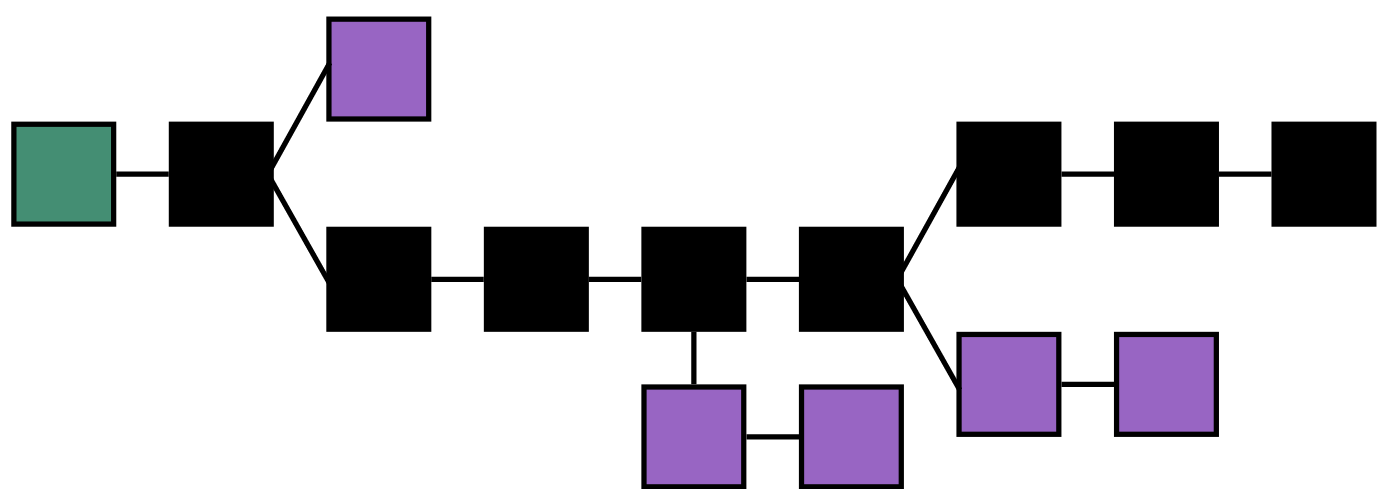
\includegraphics[scale = 0.25]{Immagini/c7f0503-reorg.png}
    \caption{Raffigurazione di una Blockchain}
    \label{fig:blockchain}
\end{figure}

Nella figura [\ref{fig:blockchain}] abbiamo in colore \textit{verde} i \textbf{genesis block}, in \textit{viola} i \textbf{orphan} e in \textit{nero} è rappresentata la blockchain composta dai nodi validi.

\subsection{Bitcoin}
Criptovaluta proposta nel 2008. nato anche per cercare di creare il sostituto digitale del denaro.
Il problema che potrebbe presentarsi riprende il \textbf{double spending}, infatti se una valuta digitale  ha un determinata firma hash collegata a un dispositivo, nulla mi vieta di copiare quella sequenza di bit e moltiplicare, virtualmente, la valuta di mio possesso e inviare la copia a una persona e mantenermi quelli iniziali io. Per evitare il problema del \textbf{double spending} si usa solitamente una \textbf{trusted third party}, per esempio la banca, che controlla e si segna i passaggi di proprietà.\\
La banca diventa però un collo di bottiglia e viene a sapere di tutti i trasferimenti di denaro, cosa che ai crittografi non piace. Nel 2008, l’idea è stata quindi quella di unire diversi protocolli crittografici e creare il bitcoin, dicendo che al posto della banca si usa un registro condiviso che tutti possono vedere dove si annotano le transazioni. \\

Le proprietà che vengono memorizzate sulla blockchain di bitcoin sono i bitcoin (BTC) o frazioni di essi (possono essere suddivisi in frazioni e sottofrazioni fino ad arrivare a $10^{-8} BTC$).\\

Le transazioni contengono diverse transazioni in ingresso, eventualmente altri campi particolare per generare nuovi bitcoin e alcuni script di transazione in output (script scritti in un linguaggio particolare). Se Alice vuole mandare a Bob un Bicoin usando il proprio client, a volta chiamato \textbf{wallet}, specifica la quantità che vuole mandare e un indirizzo. Ogni utente ha un indirizzo, che corrisponde a una lunga sequenza di numeri.  L’indirizzo si ottiene utilizzando la chiave pubblica (algoritmi a chiave pubblica). Attraverso un algoritmo opportuno, ogni utente si crea una chiave pubblica e una privata, rendendo pubblica la prima, che verrà utilizzata da chiunque voglia mandargli un messaggio.  \\
Per decifrare il messaggio l’utente utilizzerà la propria chiave privata. Dalla chiave pubblica di Bob a cui si applica una funzione di hash, Alice ottiene l’indirizzo di Bob. L’indirizzo è quindi una sorta di identità per l’utente, ma l’utente può generare tutte le copie di chiave pubblica e privata che vuole e quindi può utilizzare sempre indirizzi diversi. In seguito i bitcoin ottenuti su diversi indirizzi si possono poi combinare. \\ Ma come fa Alice a dimostrare che Lei è la proprietaria di quel Bitcoin e che quindi ha la possibilità di mandarlo a Bob? Questa transazione la firma con la firma digitale e invia la transazione a Bob. \\
La firma digitale viene applicata utilizzando la chiave segreta del mittente (Alice), al fine di dimostrare la propria identità.
I nodi P2P verificano quindi che la firma del mittente sia valida e che la somma di bitcoin mandata non sia già stata inviata ad altri, quindi che la transazione sia valida in caso positivo viene aggiunta alla blockchain. \\
Il fatto di possedere un Bitcoin è indicato dal fatto che sia possibile iniziare una transazione per mandarlo a qualcun altro e quindi che si possieda una chiave segreta, che dobbiamo salvarci essendo molto importante. 
Nelle blockchain non si registra il numero di Bitcoin posseduti dagli utenti ma la storia dei Bitcoin (i loro passaggi di proprietà) e quindi le transazioni.

\subsubsection{Miners}
I miners sono  i membri della rete P2P. \\
Esiste un pool di transazioni che vengono proposte dai vari client (\textbf{wallet}) e i miners osservano le transazioni, ne scelgono un migliaio che vengono validate e cercano di formare il nuovo blocco (circa uno ogni 10 minuti). Dopo aver validato le transazioni eseguono le operazioni computazionali collegate al cosiddetto \textbf{proof-of-work}. I miners devono dimostrare di avere effettuato una certa computazione per aver diritto di aggiungere il prossimo blocco alla catena. La computazione da fare e quindi la creazione del blocco diventa sempre più difficile. \\

Le funzioni di hash sono funzioni crittografiche che prendono in input una sequenza di bit (in teoria arbitrariamente lunga, in pratica il limite per la lunghezza è molto alto e non lo si raggiunge mai) e produce una sequenza di poche centinaia di bit (che vorrebbe essere unica). Dato che il dominio della funzione di hash è molto più grande del codominio può capire che l’hash di due file diversi produca in output la stessa sequenza di bi, in questo caso si ha una \textbf{collisione}. \\

Le collisioni esistono ma sono molto rare, e quindi si può pensare che ogni impronta (\textbf{valore della funzione id hash}) sia associata univocamente al file da cui è stata calcolata. Più difficile ancora è, dato un input con una certa impronta, trovare un altro input che abbia la medesima impronta. \\
Data un’impronta, è estremamente difficile trovare un input che produce una determinata impronta (la funzione di hash è \textbf{one-way}, ovvero facile da calcolare ma difficile da invertire). \\ 
Anche se si cambia un solo bit dell’input si ottiene un output completamente diverso, non si possono quindi cercare correlazioni statistiche o cercare di capire quale sia la regola con cui vengono calcolate. \\

Nella textbf{proof-of-work} si deve dimostrare di aver svolto una certa quantità di lavoro. Viene preso il dato di cui si deve calcolare l’hash e gli si aggiunge una certa quantità casuale, chiamata \textbf{nonce}, e si calcola l’hash di questa concatenazione.In seguito vado a vedere se il risultato ha un certo numero prefissato di bit più significativi uguali a 0, così facendo si riduce il codominio, e quindi il numero possibile di output validi in quanto devono iniziare con un certo numero di 0. Se si aumenta il numero di 0, si rende meno probabile il fatto che sparando a caso un nonce si ottenga un risultato valido. Ciò rende più difficile creare le impronte e quindi i blocchi. Al contrario se si diminuisce il numero di 0 richiesti, lo si rende più facile. \\
Quando finalmente il \textbf{miner} riesce a creare il blocco, questo viene mandato nella rete P2P e gli altri miners ne controllano la validità. Se ne riscontrano la validità il blocco viene inserito in cima ad ogni copia della blockchain.

Mentre un miner sta lavorando a un blocco B e qualcuno ne propone prima un altro B’ che viene aggiunto, il miner, per poter ancora proporre B, deve scartare le transazioni di B che già compaiono in B’ e aggiungere l’hash di B’ nell’intestazione di B. L’unico momento in cui si possono creare dei nuovi bitcoin è durante la creazione di un nuovo blocco: chi riesce ad aggiungere un nuovo blocco alla catena ha dei nuovi bitcoin. I bitcoin creabili in un blocco sono in numero limitato (se ne possono costruire al massimo 21 milioni). Il mercato delle criptovalute è un mercato non regolamentato soggetto a manipolazione.

Un problema del decentramento è l'\textbf{Attacco del 51$\%$}, infatti se si controlla, o si possiede, il 51$\%$ della potenza di calcolo di tutti i miners, si ha sempre il controllo di quale blocco viene aggiunto. Un problema ulteriore è il \textbf{problema dello spreco di energia}, si è verifiato che un tipo di confronto tutti contro tutti (tra miner) è molto inefficiente, la rete P2P che gestisce la blockchain di bitcoin consuma più dell’Argentina. Si cercano quindi algoritmi per esempio per la creazione del consenso diversi dalla \textbf{proof-of-work}, un algoritmo potrebbe essere la \textbf{proof-of-stake}.\\

Lo stake è la quantità di soldi. Non tutti fanno il mining, ma solo un sottoinsieme di nodi viene scelto per validare le transazioni. Il sottoinsieme viene scelto in maniera direttamente proporzionale alla quantità di soldi che si è deciso di bloccare (di rendere disponibile agli altri) su un conto speciale. Chi mette più soldi ha più probabilità di essere scelto. \\

Il fatto che ci sia un numero massimo di bitcoin creabili e che creali diventi sempre più difficili ha fatto paragonare i bitcoin all’oro (oro digitale).

\subsubsection{Altro esempio}
Prendiamo in considerazione il caso in cui Alice vuole dare una porzione dei bitcoin a Bob.
Se Alice possiede 10 bitcoin e ne vuole dare 1 a Bob. Allora Alice deve creare 2 transazioni una in cui a partire dall’input di 10 BTC  produce un output verso Bob e un’altra in cui contemporaneamente a partire dall’input 9 produce un output a se stessa. In sostanza Alice deve effettuare due transazioni una in cui fornisce i suoi bitcoin a Bob e una con cui si dà il resto. La somma totale data in input a Bob non dev’essere minore della somma in output (verso Alice). La somma in input può infatti essere maggiore perché la differenza tra i bitcoin totali mandati e quelli che si vogliono fare avere a Bob costituirebbe una \textbf{fees}, un compenso che viene dato al miner. \\ I miner selezioneranno per prime le transazioni del pool che hanno le \textbf{fees} più alte. Le transazioni con \textbf{fees=0}, difficilmente vengono considerate e perciò vengono dette \textbf{transazioni zombie}. \\

Per essere ragionevolmente sicuri che una transazione sia andata a buon fine si devono aspettare circa 6 blocchi (un’ora), quindi non è possibile utilizzare i bitcoin per piccole e rapide transazioni (comprare il giornale).

\subsection{Ethereum}
Un'altra tipologia di block chain in cui si pone l’attenzione non sulle transazioni, ma sulle computazioni. Non vengono memorizzate le transazioni come bitcoin, ma all’interno di Ethereum ogni utente ha un account nel quale ha una certa quantità di criptovaluta (\textbf{ether ETH}). Le transazioni avvengono esattamente come per i bitcoin.\\ 
In Ethereum c’è la possibilità di scrivere gli \textbf{smart contract}, sono il corrispettivo dei contratti tra persone (si dà in uso un bene e si chiede in cambio un compenso mensile). Gli smart contract sono scritti con il linguaggio di programmazione \textbf{Solidity}.

I contratti vengono compilati in un bytecode (linguaggio macchina della Etherum VM) e quest’ultimo viene memorizzato in tutte le copie della blockchain di Ethereum. Un client può fare una transazione in cui o trasferisce soldi o chiama una funzione all’interno di un contratto. Durante le transazioni uno dei miner raccoglie la transazione che esegue un contratto e lo esegue sulla sua macchina. Ogni esecuzione di ogni singola operazione del bytecode costa una certa quantità di \textbf{gas}, ovvero una certa quantità di soldi che si è disposti a spendere per l’esecuzione del contratto (se ne dovessero avanzare, la parte in più viene restituita). Nel caso in cui non si abbiano abbastanza soldi per eseguire un contratto, viene sollevata un’eccezione \textbf{Out of gas}: i soldi spesi vengono persi e il contratto non va a buon fine perché dà errore.
Gli smart contract sono codice lato server di cui chiunque può vedere il bytecode. I tempi di esecuzione sono lenti, parlando di un ambito molto delicato come il denaro. 

\subsubsection{Tipologie di Blockchain}
Ci sono diversi tipi di blockchain.
\begin{itemize}
    \item Permissionless: dove chiunque può scaricarsi il software e diventare miner, non ha bisogno di permessi particolari.
    \item Permissioned (publica e privata): dove i nodi della rete P2P (che sono quelli che possono scrivere, avviare le transazioni) si conoscono uno con l’altro ma non si fidano, motivo per cui scrivono pubblicamente sulla blockchain(public blockchain). 
    I miners sono potenzialmente in conflitto fra loro: ci guadagnano dalle perdite degli altri.(private blockchain)
\end{itemize}
Inoltre si può verificare la necessità di utilizzo di una blockchain e del tipo necessario. Come possiamo notare dalla figura [\ref{fig:do_i_need}]. 

\begin{figure}[H]
    \centering
    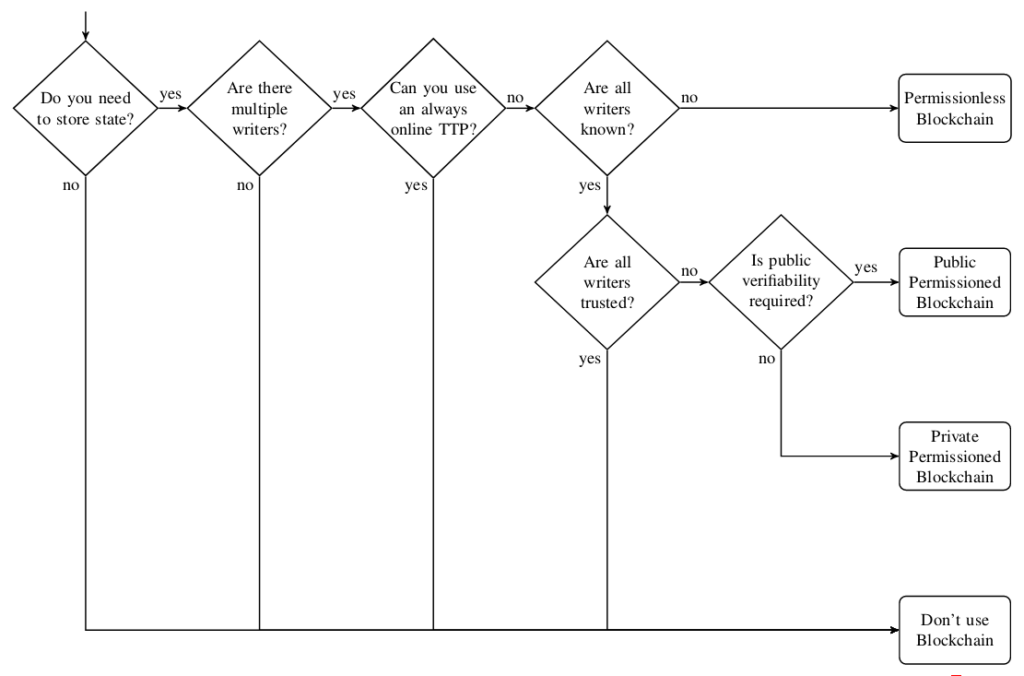
\includegraphics[scale = 0.3]{Immagini/blockchain-it-1024x676.png}
    \caption{Ho veramente bisogno di una blockchain?}
    \label{fig:do_i_need}
\end{figure}

% \section{Introduzione NoSQL}
\textbf{Quando ci chiede un modello document based, non parlare solo di MONGO-DB}\\
Nel 1970 Codd, impiegato IBM pubbluca un modello in cui presenta un modello di rappresentazione dati indipendente dall’implementazione. Si era passati dal modello gerarchico (in cui bisognava usare i puntatori per accedere ai dati) al modello relazionale. \\

Questo passaggio è stato fondamentale per lo sviluppo del mondo dell’informatica, un mondo dove l’hardware dedicato allo storage era estremamente costoso, poco capiente (nel range di pochissimi megabyte) e logisticamente parecchio ingombrante. 
Il modello relazionale quindi era studiato principalmente questo contesto, proponendo strategie per la rappresentazione compatta dei dati.\\
Principali problemi nella memorizzazione di dati: spazio occupato e tempo che ci si impiega per fare un’interrogazione.
Lo spazio ormai non è più un problema (eccetto casi particolari).\\

\subsection{Aspetti positivi del modello relazionale}
Sono diversi gli aspetti positivi del modello relazionale:
\begin{itemize}
    \item è \textbf{un modello ben definito}, quindi c'è il principio della minimizzazione e il principio della \textbf{closed world assumption}, quest'ultimo assume che tutto quello che la mia applicazione deve sapere è messo all'interno del database. Quello che ne deriva è che si ha anche l’uso del \textbf{NULL value} in caso di assenza di informazione sul valore.
    \item è \textbf{ un modello chiuso} che contiene tutto il necessario, risultava un modello ragionevole in un contesto come quello “pre anni 2000”, dove un’azienda tipicamente necessitava solo di informazioni interne all’azienda stessa. Infatti non c’erano, per esempio, le informazioni dei social network. Infatti nel post 2000 non esiste più la \textbf{closed world assumption}.
    \item \textbf{un RBDMS}, è un modello ben studiato, ha infatti più di 35 di sviluppo in sulle tematiche de della sicurezza, ottimizzazione e standardizzazione. Gode inoltre delle proprietà \textbf{ACID}. 
    Inoltre ormai talmente tante informazioni sono memorizzate tramite il modello relazionale che le aziende sono restie a cambiare modello (a causa dei rischi di perdita dei dati durante un porting (travasare i dati da una parte all’altra), considerando che i dati persi non sono possono non essere recuperabili, a meno di repliche).
    \item \textbf{modello ben conosciuto}, dovuto anche al fatto che molte aziende utilizzano ancora il modello relazionale, per il punto spiegato prima, il modello relazionale è studiato anche nelle scuole e nelle università.
    \item \textbf{costituisce la scelta migliore per diversi casi d’uso}
\end{itemize}
Tuttavia ci sono alcune limitazioni:
\begin{itemize}
    \item è un \textbf{modello chiuso}, questo è quindi sia un pregio che un difetto del modello relazionale. Il principio di minimizzazione, ai giorni nostri, va a discapito delle performance. Motivazione valida anche per dire che il principio della closed world assumption non ha più molto senso. \\
    Il modello prevede inoltre un sistema di \textbf{un solo valore per ogni attributo}, non ammettendo quindi array o altre strutture per dati con multipli valori. Diventa perciò impossibile fare interrogazioni in modo strutturato all’interno dei valori stessi, dovendo ricorrere a diversi workaround (il metodo standard utilizzato è quello di fare una tabella di join a parte, detta \textbf{tabella di part-of}, coi possibili multi-valori, portando però ad operazioni di join molto dispendiose). \\
    Un altro aspetto negativo, nel avere un modello chiuso è rappresentato dal fatto che molti linguaggi moderni sono OOP, con la \textbf{object persistency}, paradigma non supportato dal modello relazionale. Come ultimo aspetto il modello non supporta i comportamenti ciclici, comportando limiti modellistici.
    \item \textbf{sono difficili da modificare} dal punto di vista schematico (tramite alter table).  Cambiare gli schemi è complesso e comporta il fermo del database. E non sono scalabili, in quanto per garantire le proprietà ACID nei sistemi transazionali e per poter garantire il 2PC si ha un limite fisico alla scalabilità
    Dopo un certo punto di crescita i costi di organizzazione rendono impossibile l’esecuzione dei protocolli che garantiscono ACID, in ambiente distribuito.  Oggigiorno ci sono varie applicazioni, legate in primis ai social network, per le quali è impossibile mantenere certi protocolli.  Il problema della scalabilità è uno degli aspetti più limitanti, specialmente in ottica \textbf{big data}, ma non solo. 
    
    \item La \textbf{scalabilità}: I database relazionali si prestano bene alle \textbf{scale up} (scalabilità verticale), ovvero cambiare l’hardware a disposizione, utilizzandone via via di più grandi e potenti, arrivando a costi esorbitanti e al punto in cui si raggiunge il limite tecnologico, ma pochissimo allo \textbf{scale out} (scalabilità orizzontale), ovvero l’integrazione di nuove parti di hardware (comodity), a prezzo più basso, all’hardware originario (il problema consiste nel fatto che l’hardware dedicato storicamente ai db relazionali non prevede questa possibilità).

    Oggigiorno si hanno sempre più spesso le architetture a microservizi (che implementano bene lo scale out).
    
    \item \textbf{Il time in market}, ovvero il tempo in cui un applicativo resta in commercio, è sempre più ridotto, portando a rendere obsoleto il processo in cui normalmente si integrano i db relazionali. Anche il time to market, ovvero il tempo di preparazione si è ridotto.
\end{itemize}


Il termine NoSQL è stato coniato da Carlo Strozzi nel 1998, inventandosi una sorta di API per Linux per accedere ai dati relazionali senza usare SQL (no SQL). Il termine è stato ripreso nel 2009 con la logica Not Only SQL, dopo che per circa 9 anni, a partire dal 2000, erano nati nuovi modelli.\hfill 

NoSQL è un'insieme di modelli di rappresentazione dati e relativi software di gestione. 
Caratteristiche fondamentali:
\begin{enumerate}
    \item tutti i modelli sono schema free o schemaless
    \item tutti i DBMS NoSQL usano il CAP theorem
    \item si passa da ACID a BASE ovvero: \textbf{B}asic \textbf{A}vailable, \textbf{S}oft state, \textbf{E}ventual consistency
\end{enumerate}

\subsubsection{Schema free}
Nel modello relazionale viene prima definito il modello, ovvero l’insieme degli attributi che descrivono i dati e le varie relazioni, e poi viene popolato con i dati veri e propri. Questo comportava che se durante lo sviluppo ci si accorgeva che bisognava aggiungere, ad esempio, un attributo bisognava modificare l’intero schema (nonché i dati già caricati). \\

Con NoSQL il modello non esiste a priori ma si basa sui dati che vengono inseriti (scheme free), quindi di fatto per ogni riga si ha potenzialmente uno schema diverso. Questo concede una grandissima libertà di sviluppo, al costo di un’alta probabilità di inconsistenza tra i dati.  \\
Tutti i modelli NoSQL assumono l’open word assumption, secondo la quale, in assenza di un dato, non vengono utilizzati i valori NULL  (che vengono eventualmente messi solo per motivi applicativi) , garantendo una grande flessibilità (che può però generare problemi). Tale flessibilità ha un costo anche dal punto di vista delle query, in quanto non si può partire dallo schema ma si deve partire da frammenti del modello. \\ 
Si ha però il guadagno che in caso di aggiunta di attributi, non bisogna modificare l’intero schema, anche se ovviamente serve una governance più forte del dato (in quanto può anche succedere che il tipo di dato non sia vincolato).

\subsubsection{CAP Theorem}
Teorema essenziale, proposto da Gilber e Lynch nel 2002 che dimostra la Congettura sulla consistenza, disponibilità e partizionamento dei webserver del 2000 di Brewer:
Preso un sistema distribuito di nodi si considerino tre aspetti:
\begin{itemize}
    \item Consistency (consistenza): tutti i nodi hanno gli stessi i dati nello stesso istante (è diverso dalla consistenza di ACID (vincoli di tipo relazionale uguali)).
    \item Availability (disponibilità): garanzia che ogni richiesta ricevuta da un sistema riceva una risposta, sia in caso di fallimento che di successo (non si deve avere quindi un’attesa infinita). Ogni client può sempre leggere e/o scrivere.
    \item Partition tolerance (partizionamento): il sistema deve continuare ad operare anche se si hanno perdite di messaggi o fallimenti di parti del sistema.
\end{itemize}
Il Cap theorem garantisce che tra queste tre caratteristiche, in un sistema distribuito, se ne possano soddisfare contemporaneamente solo due su tre. I DDBMS per esempio rinunciano alla partition tolerance, garantendo le prime due caratteristiche (CA) (anche se con un numero limitato di nodi si può arrivare ad avere un CAP).
I sistemi NoSQL sono tipicamente o CP, non potendo garantire che il DBMS lavori 24/7, o AP, non potendo garantire che i dati siano sempre consistenti.  \\ 
Non è detto che due db NoSQL che implementano lo stesso modello garantiscano le stesse due caratteristiche CAP. Quindi in fase progettuale la scelta tra due delle caratteristiche CAP è un punto chiave per poi scegliere eventualmente su che DBMS NoSQL appoggiarsi.\\
In fase progettuale si hanno 3 scelte da effettuare: modello, DBMS e caratteristiche del CAP theorem.

\subsubsection{Base principal}
Basic Availability: comunque vada, la risposta viene sempre data anche nel caso di consistenza parziale.
\begin{itemize}
    \item Soft state: si rinuncia al concetto di consistenza di ACID.
    \item Eventual consistency: prima o poi i dati convergeranno ad uno stato di consistenza (in opposizione alla consistenza immediata di ACID).
\end{itemize}
\subsection{Modelli NoSQL}
\begin{itemize}
    \item key-value stores: modello chiave-valore, semplice da memorizzare, e utile per il caching.  Il valore è un blob, quindi non si ha modo di interrogare internamente il valore, ma deve essere l’applicazione a manipolarlo. Il mapping chiave-valore è supportato da meccanismi di hash, per massimizzare le performance. Viene garantito l’hashing distribuito, ovvero la distributed hashed table.
    \item column family stores: la chiave punta a colonne multiple di valori, ottenendo un formato pseudo-relazione. Ogni riga, in questo schema wide column, ha una sua struttura interna diversa da quella di altre righe, che sono comunque indipendenti. La chiave ovviamente può essere hashata. Non si può fare ranged query.
    \item document databases: formato da documenti con coppie chiave-valore o chiave-oggetto, dove l’oggetto può anche essere un’altra chiave-valore, un array di valori o un array di oggetti. Nel modello documentale si ha un elemento più importante, detto root che ha al di sotto tutti gli altri.
    \item graph databases: con nodi e relazioni tra gli stessi (archi). I nodi possono rappresentare entità a cui sono associate varie proprietà (property graph), che sono quindi pertinenti ai nodi. I graph db non scalano bene.
    \item RDF databases
\end{itemize}

Il tipo di modello più complesso è anche il meno voluminoso e scalabile e viceversa. 
Il problema fondamentale in tutti i modelli è come connettere le informazioni e questo diventa un problema fondamentale in termini di prestazioni e analisi da effettuare. 
Le relazioni sono implicitamente incluse nei dati. 
La scelta del modello dipende dall’applicativo e ci sono applicativi che possono obbligare ad avere due o più modelli.
Ogni vendor ha il suo linguaggio di query per il suo DBMS NoSQL.

% \section{Document Based System}
Il document based system consiste in un’evoluzione del modello chiave-valore, in quanto si ha una chiave, ovvero un \textbf{object identifie}r, che può essere indicizzata tramite un meccanismo di hashing. I documenti solitamente vengo memorizzati in file JSON o XML e possono essere cercati a qualsiasi livello.\\
Il modello documentale, a differenza del modello relazionale, ha una struttura ad albero e quindi l’accesso ai dati deve partire dal nodo radice e scendere verso le foglie (anche se si può avere un accesso a indici per accedere alle informazioni necessarie). Si ha quindi il concetto di elemento più importante degli altri (quello nella radice); concetto assente nel modello relazionale definibile pertanto un modello “piatto” (ad eccezione delle data warehouse dove si ha effettivamente una tabella principale).\\
La rappresentazione documentale è più vicina al pensiero umano in quanto a suddivisione in cartelle per varie tipologie di informazioni.

Caratteristiche del modello documentale:
\begin{itemize}
    \item è multidimensionale, ad albero
    \item ogni campo può contenere zero valori, un valore, valori multipli o altri documenti
    \item si possono effettuare query ad ogni campo e in ogni livello
    \item lo schema è flessibile: due documenti della stessa collezione possono avere uno schema diverso di rappresentazione dei dati
    \item si possono aggiungere “in linea” nuove informazioni
    \item gli elementi sono legati tra loro nei documenti e pertanto sono richiesti molti meno indici per effettuare le query. 
    Ciò permette di avere performance migliori non dovendo, come nel caso relazionale, prendere $n$ tabelle in $n$ file diversi nel filesystem e effettuare poi il join.
\end{itemize}
Il modello documentale permette due tecniche principali:
\begin{enumerate}
    \item \textbf{referencing}: come per il modello relazione, si relazionano due documenti tramite un certo attributo.
    \item \textbf{embedding}: si aggiunge quello che nel \textbf{referencing} è un secondo documento come specifica di un certo valore, aggiungendo quindi un livello di profondità.  Ciò va ad aumentare lo spazio utilizzato, ma non è più un problema.
\end{enumerate}

A causa del \textbf{time to/in market} sempre più ridotto, ormai quasi ogni applicazione ha il suo db e questo obbliga ad avere una certa flessibilità dello schema.
Questa flessibilità garantisce che una modifica allo schema (un’aggiunta o modifica degli attributi) non sia un problema (come sarebbe per un modello relazionale). 
Questa flessibilità però comporta che in fase di query non si abbia uno schema prefissato tramite il quale interrogare (e non si possano nemmeno vedere i primi $n$ documenti per dedurre lo schema in quanto l’$n+1$ potrebbe essere comunque diverso). Questa problematica la si riscontra soprattutto nel caso in cui si utilizzi un database costruito da terzi.

Non si ha più un unico linguaggio di query come per i modelli relazionali (SQL), ma uno per vendor (tra cui jsoniq, jmespath, jaql, JLINQ).

\subsection{Mongo DB}
\textbf{MongoDB} è un DBMS non relazionale documentale che memorizza i dati in un modello chiamato binary json (\textit{Bson}), che consente maggior efficienza tramite una rappresentazione binaria. Tramite l’embedding dei dati consente di non eseguire i join e permette anche l’accesso tramite indici. Supporta comunque il referencing anche se con cali di performances.\\
Dal punto di vista architetturale si hanno una serie di engine diversi fra loro (attualmente si usa WiredTiger (WT)). Grazie a WT si è introdotto, nella v4, il supporto alle transazioni. \\
Si ha poi il data model, il MongoDB query language (MQL) (che è proprietario), i componenti di controllo degli accessi e il meccanismo di gestione. 
Le repliche sono organizzate in replicaSet. \\
Esempio di schema in Mongodb: 

\begin{lstlisting}
var p = {
    '_id': '342',
    'author': DBRef('User',2),
    'timestamp': Date('26-10-20'),
    'tags': ['MongoDB','NoSQL'],
    'comments':['author': DBRef('User',4),
                'date': Date('26-10-20'),
                'text': 'hello',
                'upvotes': 7,...]
}
>db.posts.save(p);            
\end{lstlisting}
Nell'esempio osserviamo la definizione di $p$ come un oggetto json. Tra gli elementi che la compongono c’è $tags$ che contiene un array di valori; mentre $comments$ è un array di documenti.
Nell’ultima riga notiamo una delle chiavi di successo di Mongodb in quanto ha un linguaggio simile a quelli di programmazione. Nel dettaglio si ha il caricamento del documento $p$ nella collezione $posts$. Si ha un meccanismo simile alla OOP e l’integrazione coi linguaggi di programmazione è facilitata dall’ormai molto diffuso supporto ai json.\\
Si possono inoltre fare indici, tramite ensureIndex (che prende come argomento un json), a ogni campo del documento e a qualsiasi livello (sono possibili indici a documenti, a array o indici geo-spaziali).
\begin{lstlisting}
  >db.posts.ensureIndex({'author': 1});      
\end{lstlisting}

\subsubsection{Replicazione in MongoDB}
MongoDB rientra nella categoria CP del \textbf{CAP theorem}, non garantendo disponibilità in caso di guasto.
La replica viene effettuata in modalità master-slave: nel gergo di MongoDB primary-secondary, dove la scrittura avviene sul primary e la replica sui secondary. \textbf{In realtà uno dei nodi replica viene definito a posteriori primary}.
Si procede per repliche parziali incrementali: all’inizio il nodo fa un sync, prendendo tutti dati dal primary e solo gli ultimi $n$ movimenti dal file di log del primary.
La garanzia della tolleranza viene garantita tramite il meccanismo di elezione dei nodi, nel caso in cui il nodo primary vada down.
Si ha che un nodo può assumere uno dei seguenti stati:
\begin{itemize}
    \item \textbf{STARTUP}: un nodo che non è membro effettivo di nessun replica set.
    \item \textbf{PRIMARY}: l’unico nodo nel replica set che accetterà le operazioni di lettura.
    \item \textbf{SECONDARY}: un nodo che può effettuare la sola replicazione dei dati (può essere promosso a PRIMARY in fase di elezione).
    \item \textbf{RECOVERING}: un nodo che sta effettuando una qualche operazione di recupero dei dati, magari dopo un rollback (può essere promosso a PRIMARY in fase di elezione).
    \item \textbf{STARTUP2}: un nodo che è appena entrato nel set (può essere eletto a PRIMARY).
    \item \textbf{ARBITER}: un nodo non atto alla replicazione dei dati, ma con lo scopo di prendere parte alle elezioni per promuovere i nodi a PRIMARY (può essere eletto a PRIMARY in fase di elezione).
    \item \textbf{DOWN/OFFLINE}: un nodo irraggiungibile.
    \item \textbf{ROLLBACK}: un nodo che sta svolgendo un rollback per cui sarà inutilizzabile per le letture (può essere promosso a PRIMARY in fase di elezione).
\end{itemize}
Se il nodo primario è riconosciuto come down dalle altre repliche si effettua una elezione e viene scelto quello con la versione più aggioranta dei dati.

\subsection{Elezioni}
L’elezione consiste nell’eleggere il nodo con la versione più aggiornata dei dati.
In questa fase le scritture sono interrotte (motivo per cui non è garantita la A di CAP), l’elezione dura comunque pochissimo. Durante il processo di elezione ogni replicaSet manda un “hearbeat” (ovvero un bit ogni due secondi) agli altri nodi. L’invio di un heartbeat dà inizio a un timeout, in modo che si possa assumere che un nodo sia down nel caso in cui scada senza aver ricevuta una risposta. Se il nodo primario risulta down si procede con l’elezione, che in termini umani è di tipo maggioritario con liste bloccate. \\
Ogni nodo ha un identificativo con un punteggio rappresentante la priorità nelle elezioni (più alto più probabile che venga eletto). Quindi appena il primary va down il secondario con valore più alto viene promosso come nodo primario e richiederà nuove elezioni rispetto agli altri. 
Si ha che un replica set può avere al massimo 50 membri di cui solo 7 votanti, che esprimono un solo voto. I nodi SECONDARY non votanti hanno priorità 0 e accettano solo operazioni di lettura. Esistono nodi a priorità 0 che sono invece votanti.
Nel caso di partizionamento della rete si rischia di avere più di un primary eletto e quindi un conseguente problema di riconciliazione, dovendo quindi bloccare la scrittura.

\subsection{Scrittura}
La scrittura avviene sul nodo primario e si hanno diverse politiche tramite l’opzione \textbf{writeConcern} che dice cosa fare per le \textbf{replicaSet}. 
Si hanno tre parametri:
\begin{enumerate}
    \item $w$: numero di nodi in cui il dato deve essere replicato prima di essere considerata conclusa l’operazione, ovvero numero di nodi sui quali deve essere confermata la scrittura per essere confermata a livello globale.
    \item $j$: intenzione di scrivere sul log di WiredTiger, tramite la logica write ahead logging (prima si scrive sul file di log e poi sul disco), prima che l’operazione sia stata eseguita. Questo per garantire la persistenza del dato, avendolo comunque nel file di log. Senza l’opzione lo scriverà in un secondo momento.
    \item $wtimeout$: tempo limite, espresso in ms, da aspettare nel caso in cui $w>0$ (se $0$ non si attende alcuna risposta prima di concludere l’operazione).
\end{enumerate}
Aumentare $w$ comporta aumentare il tempo di esecuzione. Nel dettaglio:
\begin{itemize}
    \item $w=0$: non da alcuna certezza di inserimento, utile per operazioni veloci.
    \item $w=1$: implica la scrittura sul nodo primary.
    \item $w=n$: implica la scrittura su $n$ nodi.
    \item $w=majority$: almeno la metà dei nodi più 1 deve aver scritto prima della conferma dell’operazione (nella realtà si tenta di scrivere su più nodi ma appena si ha un ack dalla metà più 1 si conferma la scrittura anche se magari si sta ancora scrivendo su altri nodi).
\end{itemize}
Qualora si debba caricare una gran quantità di dati, di cardinalità conosciuta, per motivi di efficienza non conviene aspettare che il nodo dia l’ack ma si caricano tutti i dati subito sul primary, controllando poi con `count` se è stato caricato tutto.

\subsection{Frammentazione}
Si hanno 3 tipi di sharding per la scalabilità orizzontale:
\begin{itemize}
    \item \textbf{hash-based}: sulla chiave
    \item \textbf{range-based}: in base ad un certo range di elementi
    \item \textbf{tag-aware}: in base a certi attributi
\end{itemize}
Si ha un meccanismo dinamico basato su\textbf{ pay as you go}, quindi nel momento in cui si ha lo sharding è MongoDB ad adattarlo ogniqualvolta cambia il volume di dati, effettuando un bilanciamento automatico. \\
Si ha uno spazio della chiave di shard divisibile in $n$ chunks per $n+1$ chiavi di shard. 
Il numero massimo di \textbf{chunk} che è possibile definire su una sharded key può definire il numero massimo di shard in un sistema.

Si hanno 3 ruoli fondamentali nella frammentazione:
\begin{itemize}
    \item mongos: punto di accesso software per le query, entry point del cluster: tutte le query verranno eseguite su questo processo. Appena lanciato mongos va a leggere il config server.
    \item config server: server che ospitano i file di configurazione che conosce la struttura degli shard, conoscendo frammentazioni e repliche. Dalla versione 4.0 ogni nodo distribuito è anche replicato.
    \item shard: istanze di MongoDB.
\end{itemize}

Quindi il router quando riceve una query capisce dove sono i frammenti, grazie al config server, e quindi procede con la query di tipo:
\begin{itemize}
    \item target query: se deve interrogare solo un nodo
    \item broadcast query: se deve interrogare più nodi
\end{itemize}

Sia gli shard che il config server sono replicati su replicaSet per evitare che diventino single \textbf{point of failure} (anche per questo dalla 4.0 ogni volta che frammento replico).
Si ha un primary shard, che contiene l’intero db (ovvero tutte le collezioni) e i secondary shard che contengono frammenti e repliche di alcune collezioni. 
Solitamente si ha quindi una configurazione a 3 nodi: un primary e due nodi secondari con frammenti diversi e le repliche del primary.
\subsection{Letture}
Ho una politica di \textbf{readConcern} (che deve essere consistente con il \textbf{writeConcern}, scegliendo anche in base a quale delle due azioni è la più dispendiosa):
\begin{itemize}
    \item \textbf{local}: valore di default per leggere i dati dai nodi in un \textbf{replicaSet}. La query è fatta secondo la località spaziale e quindi se legge un nodo non primary si rischia di leggere dati non ancora replicati.
    \item \textbf{available}: valore di default per lettura su nodi secondari. Fa vedere che il dato c’è ed è consistente.
    \item \textbf{majority}: valore utilizzato quando serve che almeno metà più 1 repliche abbiano ricevuto un ack in scrittura sul dato per poter leggere.
\end{itemize}
\subsection{Query Mongo Document}
\begin{minipage}{.50\textwidth}
\begin{lstlisting}[caption = Scrittura in MongoDB]
db.user.find({
	age:{$gt:18},
	name:1,
	address:1
}).limits(5)
\end{lstlisting}
\end{minipage}\hfill
\begin{minipage}{.50\textwidth}
\begin{lstlisting}[caption = corrispettivo in SQL]
SELECT name, address
  FROM user
  WHERE age>18
  LIMIT 5
\end{lstlisting}
\end{minipage}

Non si hanno le stesse rappresentazioni matematiche, si usano infatti i Query operators abbiamo quindi:\\
$gt$ = greater than, questo perché si usano identificativi per i confronti (per non utilizzare i simboli $>$, $<$ che darebbero fastidio nelle stringhe). Abbiamo usato inoltre $.limit()$ che ci permette di rappresentare i top 5 elementi complicati del nostro esempio. \\
Vediamo le varie operazioni:


\begin{minipage}{.50\textwidth}
\begin{lstlisting}[caption = operazione di Insert]
db.user.insertOne({
    name: "Andrea" ,
    age: 26,
    Teach[<datawarehouse>, <architecture>]
  })
\end{lstlisting}
\end{minipage}\hfill
\begin{minipage}{.50\textwidth}
\begin{lstlisting}[caption = operazione di Update]
Db.user.updateAll({
    name:{$eq: <Andrea>},
    {$set: {Role: <PA>}},
    {$upsert:true}
})
\end{lstlisting}
\end{minipage}
Usando insertOne si specifica che si vuole inserire un solo documento mentre usando insertAll si specifica che si vogliono inserire tutti i documenti.\\
Il comando $upsert$ invece corrisponde a un \textbf{insert if not exist}, per permettere l’inserimento in caso di assenza e la modifica in caso di presenza del dato. Tale cosa è assente in SQL, è necessario un doppio comando.

\subsection{Importazione dei dati}
Si hanno varie utility per importare i dati, da specificare come opzioni al comando\\ \textbf{mongoimport}: mongoimport –d database –c collection –type csv -ignore blanks –file PATH (per importare un csv al path PATH ignorando gli spazi bianchi).

\subsection{Transazioni}
Dalla versione 4.0 MongoDB ha introdotto nel modello documentale le transazione tramite l’engine Wiredtiger. Viene quindi introdotto il concetto di log per il quale tutto è nel nodo primary. \\
Si opera sempre sul nodo facendo un lock che può essere di tipo:
\begin{itemize}
    \item \textbf{sharded} (S): per le letture
    \item \textbf{exclusive} (X): per le scritture
    \item \textbf{intent sharded} (IS): per esprimere l’intenzione di bloccare in modo condiviso uno dei nodi che discende dal nodo corrente
    \item \textbf{intent exclusive} (IX): per esprimere l’intenzione di bloccare in modo esclusivo uno dei nodi che discende da quello corrente 
    \end{itemize}
Il lock garantisce transazioni a livello di singola collezione, mentre prima l’atomicità era garantita a livello della singola operazione. \\
Nel caso del \textbf{referencing} invece serviva una gestione più approfondita delle transazioni. Essendo WT creato originariamente per un sistema distribuito funziona solo per sistemi distribuiti, infatti avendo un solo nodo si presuppone che si abbia una sola applicazione che accede, cosa che renderebbe a priori più semplice la gestione.

\subsection{Efficienza}
Spesso il cambiamento del modello può comportare un miglioramento delle prestazioni non indifferente, più del cambiamento di hardware. Avere documenti separati più piccoli migliora il tempo, rendendolo lineare (mentre un grosso documento embedding ha tempi esponenziali nell’inserimento delle righe).
Con questa soluzione poi bisogna poi sistemare le query.
% \section{Graph DB}
Il grafo lo conosciamo, si ripresenta nella solita forma $G = (V,E)$, è infatti una collezione di nodi e archi. Diremo quindi che un grafo è un insieme di nodi e di relazioni fra loro, dove al suo interno i concetti più importanti, quelle che nel modello relazionale erano chiamate Entità, vengono ora modellate come nodi. Il nodo con cui le entità sono semanticamente associate si modellano come relazioni, tramite archi. \\
I grafi possono essere applicati in diversi ambiti:
\begin{itemize}
  \item social network
  \item sistemi di raccomandazione, che suggeriscono oggetti simili a utenti simili
  \item ambito geografico
  \item reti logistiche (per spedizione dei pachi ad esempio)
  \item transazioni finanziarie per la \textit{fraud detenction} (riconoscendo certi pattern sospetti, anche a livello geografico)
  \item master data management, rappresentazione unica della realtà
  \item bioinformatica
  \item controllo di autorizzazioni e accessi
\end{itemize}
Ci sono due modi per descrivere i dati, esistono :
\begin{itemize}
  \item \textbf{descrizione estensionale dei dati} quando si descrivono le istanze via-via, descrivendo anche istanze di tipo diverso (magari utenti e messaggi) usando la stessa sintassi del nodo (ugualmente per gli archi). La semantica viene data dall'etichetta
  \item \textbf{descrizione intensionale dei dati}, che bisognerebbe inferirla  direttamente dai dati e quindi non è applicabile
\end{itemize}


Nei RDBMS si ha il \textit{join} basato su valori, facendo uno \textit{scheme understanding} sulle varie tabelle, ottenendo quindi il risultato tramite anche più operazioni di \textit{join}. Si può avere però il problema applicativo, avendo magari \textbf{relazioni ad anello} tra le varie tabelle ad esempio una tabella persona che tramite una tabella amici ritorna su se stessa, avendo la tabella amici che esplode in numerosità. Si hanno potenzialmente livelli infiniti di \textit{join} si va incontro al \textbf{join bombing}, che fanno soffrire i DBMS. 

Notiamo che nei sistemi a grafo ora abbiamo gli archi, per collegare i nodi contenenti informazioni, mentre nei documentali avevamo identificatori che puntavano ad altri documenti: solitamente con un modello basato sui valori come se fossero \textit{foreign keys} dei RDBMS). Nei document based io devo definire un ordine gerarchico, devo fare un albero, e quinid i task di modellazione risultano molto complessi, con scarsa efficienza e complessità nel gestire dati fortemente connessi, mentre, con il referencing starei simulando una sorta di modello a grafo. \\

Un aspetto importante dei DB a grafo è che hanno forte potenza espressiva permettendo di caratterizzare i nodi con un certo \textit{tipo}, che possiamo chiamare etichette per caratterizzare il nodo, e definire le varie relazioni tramite archi.
\begin{figure}[H]
    \centering
    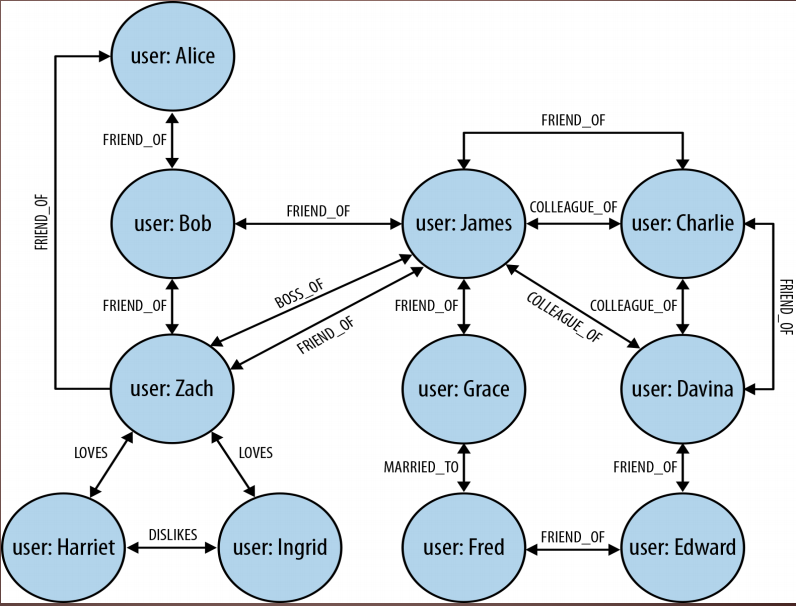
\includegraphics[scale = 0.4]{Immagini/slide-14-graphdb.PNG}
\end{figure}
Nei nodi posso rappresentare anche entità complesse, con vari attributi, ovvero varie \textbf{proprietà}. Ovviamente ogni nodo può avere un set di attributi diversi, avendo fortissima libertà di schema.\\
È un modello molto più immediato rispetto ad un RDBMS. Inoltre, nel caso si abbiano potenzialmente più relazioni tra due nodi basta contare quanti cammini orientati, che possono quindi passare per nodi intermedi diversi, esistono tra quei nodi per ottenere la cardinalità di tali relazioni. \\

Posso anche rappresentare un \textbf{property graph} in diversi modi:
\begin{itemize}
  \item quando sia nodi che relazioni possono avere proprietà espresse da chiave-valore, accettando quindi che i nodi abbiano un tipo
  \item altri ammettono array di valori
\end{itemize}
Si nota che invece in altri modelli NoSQL come RDF i nodi possono avere un tipo ma non proprietà e le relazioni non hanno proprietà, dovendo sempre rappresentare il tutto tramite triple \textbf{soggetto-predicato-oggetto}. \\
Il problema di modellazione dei grafi si ritrova quindi nella scelta di cosa mettere come nodo e cosa come relazioni (ed eventualmente le proprietà), avendo varie scelte modellistiche con vari pro e contro.\\ 
Anche nel caso dei GraphDB ogni vendor ha il suo linguaggio, anche se ne esiste uno \textit{standard}, chiamato \textbf{Gremlin}, che più che essere un linguaggio di interrogazione è un \textit{linguaggio di attraversamento dei grafi}. Questo tipo di linguaggio viene detto \textbf{vertex-based} che si usano per studiare la validità di predicati tramite l'attraversamento dei nodi.\\
\begin{enumerate}
  \item \textbf{graph processing}, dove ci si concentra sul processamento dei dati, processamento che viene eseguito tramite i grafi 
  \item \textbf{graph storage}, dove i dati vengono memorizzati in forma di grafo 
\end{enumerate}

In entrambi i casi la cosa può essere fatta in modo:
\begin{itemize}
  \item \textbf{nativo}:  \textit{native graph storage} per indicare che sono ottimizzati e progettati per le gestione stessa dei grafi. In questo caso comunque i dati vengono memorizzati in modo intelligente, memorizzando in modo vicino i nodi e il loro archi, facendo \textit{index free adjacency}, in modo che seguire gli archi uscenti da un nodo è molto più immediato.
  \item \textbf{non nativo}: \textit{non native graph storage} per indicare che i dati vengono trasformati da grafo ad un formato diverso tra cui relazionale, object oriented db. Si rischia comunque il \textit{join bombing}
\end{itemize}

Si hanno quindi due approcci principali per gestire un grafo:
\begin{itemize}
  \item \textbf{graph database}, ovvero un DBMS che gestisce in maniera persistente un grafo che viene usato per le transazioni. Si usa la dicitura OLTP
  \item \textbf{graph compute engine}, ovvero tecnologie per l'analisi \textit{off line} dei grafi. Si usa la dicitura OLTP
\end{itemize}

I graph database supportano le operazioni CRUD (come tutti i modelli NoSQL): \textbf{C}reate, \textbf{R}ead, \textbf{U}pdate e \textbf{D}elete.

Come abbiamo visto si studiano gli attraversamenti del grafo per fare le query in modo performante non facendo join ma attraversando e basta. Sono inoltre costruiti per essere usati nei sistemi transazionali (OLTP), per dati compessi e connessi. \\ 

Abbiamo detto che per i sistemi nativi sono ottimizzati per i grafi e vengono poi discussi in seguito. Ci sono poi i grafici non nativi che trasformano i dati in un grafo relazionale object oriented. 
Si ha un problema grave coi grafi: \textbf{i grafi non scalano bene e non possono essere facilmente frammentati}.\\ Partizionare un grafo raramente è possibile, in quanto comporta un taglio di relazioni. Se quindi si vuole scalare bisogna passare, alla fine, ad un altro modello, aggiungendo però costo di comunicazione tra il modello a grafo e il nuovo modello scelto, aggiungendo un layer software.\\

Il sistema fondamentale dei \textbf{native graph storage} memorizzano in modo vicino i nodi e il loro archi, facendo \textit{index free adjacency}, in modo che seguire gli archi uscenti da un nodo è molto più immediato.

\subsection{Neo4j}
Abbiamo già introdotto precedentemente Neo4j. Sappiamo che è nativo sia per il \textit{graph processing} che per il \textit{graph storage} .\\

Approfondiamo quindi il \textbf{linguaggio di interrogazione di Neo4j}, chiamato \textbf{Cypher} (\textit{OpenCypher} nella versione open).\\ 
Cypher è definito come un \textbf{pattern-matching query language}. È un linguaggio simil-umano, espressivo, dichiarativo (si dice il cosa e non il come), che consente operazioni di aggregazione, sorting e di limit e permette di aggiornare il grafo.\\ Un formato in modo testuale viene rappresentato con le parentesi tonde per i nodi e le quadre per gli archi. Le relazioni orientate vengono indicate tramite $->$ o $<-$.
Per esempio \\ $(c)-[:KNOWS]->(b)-[:KNOWS]->(a), (c)-[:KNOWS]->(a)$, possiamo rappresentare in questo modo una lista di amici. \\ Con la virgola $,$ andiamo a rappresentare una $\land$. Un modo equivalente di rappresentazione della stessa query :\\
$(c)-[:KNOWS]->(b)-[:KNOWS]->(a)<-(c)-[:KNOWS]$
Vediamo quindi un'interrogazione classica in Cypher, dove si cercano tutti gli utenti tali per cui conosce qualcuno $a$ che conosce qualcuno $b$ e che sono etichettati come \textbf{Michael}, ritornando $a$ e $b$: 
\begin{lstlisting}
    MATCH(c:user)
    WHERE (c)-[:KNOWS]->(b)-[:KNOWS]->(a),
          (c)-[:KNOWS]->(a), c.user="Michael"
    RETURN a, b
\end{lstlisting}
Il risultato sarà una \textbf{tabella} che contiene tutte le coppie $a$ e $b$. Avrà dei dati ridondati a causa della dualità intrinseca di avere $a$ che conosce $b$, cosa che probabilmente porta ad avere che $b$ conosce $a$. \\
Quindi il risultato \textbf{non sempre} è un grafo (mentre nel documentale era sempre un documento e nel relazionale una tabella) ma può anche essere altro, ad esempio una tabella. Non è quindi sempre possibile concatenare query in quanto potrei non avere un grafo in uscita.\\
Si hanno delle clausole nel linguaggio Cypher:
\begin{lstlisting}
    WHERE 'per imporre criteri di filtraggio tramite pattern-matching dei risultati'
    CREATE / CREATE UNIQUE 'per creare nodi e relazioni'
    DELETE 'per cancellare nodi, relazioni e propriet\textnormala'
    SET 'per impostare dei valori alle proprieta'
    FOREACH 'per fare un update per elementi del grafo posti in una lista '
    UNION 'per unire i risultati + query'
    WITH 'per concatenare query propagando i risultati in pipe'
\end{lstlisting}


\textbf{Qui fa un esempio che personalmente poco mi interessa cosa? inutile}

Abbiamo già visto che non ha meccanismi nativi di frammentazione, avendo scelto di sfruttare la \textit{index free adjacency} e la modellazione a grafo, non permettendo scalabilità. In compenso garantisce però
\begin{itemize}
  \item permette le transazioni con tutte le proprietà ACID, con meccanismi di locking
  \item garantisce la recoverability
  \item garantisce la disponibilità
  \item garantisce la scalabilità, infatti nonostante le limitazioni, garantisce l'\textbf{alta disponibilità}.
\end{itemize}
Per la scalabilità l'idea è che è possibile andare a definire un cluster di nodi Neo4j, alcuni chiamati \textbf{core server}, ovvero nodi per cui tutte le scritture sono fatte in contemporanea, essendo quindi sincronizzati. Si hanno poi gli altri nodi che sono chiamati \textbf{replica server}, che sono di sola lettura e vengono anche usati per reporting analysis etc$\ldots$. Fatta una query essa comunque non viene distribuita ma eseguita sul nodo più vicino. Tutto questo sistema è detto \textbf{casual clustering}.\\ 
Si ha una bassa \textbf{latenza} nelle query in quanto si usa un indice per risalire al primo nodo e poi si procede coi cammini, avendo quindi che le performances non dipendono dalla grandezza del dataset ma solo da quali sono i dati richiesti dalla query.\\

In situazioni reali, ad esempio un e-commerce, posso avere i dati salvati in vari DBMS, sia relazionali che NoSQL, a seconda dei dati che contengono. Dover gestire tutti questi modelli diversi è molto complicato, ma sensato in base al tipo di dati. Ho quindi una sorta di \textbf{mondo poliglotta}. 
\subsection{ArangoDB}
In questo mondo poliglotta complesso ci arriva in soccorso un particolare DBMS: \textbf{ArangoDB}.\\ 
Il DBA dovrebbe conoscere tutti i modelli in uso e tutti i linguaggi associati, essendo anche in grado di gestire i vari conflitti. ArangoDB introduce il concetto di \textbf{db poliglotta}, supportando i modelli: \textbf{chiave-valore}, \textbf{document based}, \textbf{graph db} e \textbf{ricerca full text}.

Rispetto ai modelli a grafo con storage non nativo il linguaggio di query di ArangoDB, chiamato \textbf{AQL (\textit{Arango Query language})}, garantisce la possibilità di interrogare dati in formato: json quindi in maniera documentale, a grafo, in formato key-value o  usando full text search. \\

\textbf{Avviso: non si è soffermato è roba accenata ma non nel dettaglio}
Ad alto livello Arango organizza i dati in database e collezioni, dove le collezioni memorizzano documenti o similari. I documenti, come già accennato, sono documenti json annidati.\\
\textbf{Qui inoltre fa solamente un esempio, anche questo non credo serva}\\
Possiamo comunque interrogare usando il modello a grafo e tali query mostrano quali documenti sono collegati (direttamente o indirettamente) ad altri documenti, specificando il cammino per ottenere il collegamento. Queste connessioni tra documenti sono chiamate \textbf{edges} che sono salvati in edge collections. Gli \textit{edges} hanno sempre due attributi che si riferiscono ai nodi entranti e uscenti: $_from $ e $_to$.

Si hanno vari metodi di scalabilità, avendo le modalità di deploy: a singola istanza, master/slave, active failover, cluster e multiple datacenters.

\subsection{Active Failover}
Nel modello master/slave quando il master fallisce lo slave non può essere sostituito e quindi si è pensato al modello \textbf{active failover}. 
In questo modello esistono delle istanze \textit{single-server} chiamate \textbf{leader} che sono in lettura e scrittura, ed esistono delle istanze, sempre \textit{single-server}, chiamate \textbf{followers} che non sono altro che vecchi slave passivi e non scrivibili.
Il leader invia le operazioni di scrittura ai followers che replicano in modo asincrono i dati tramite la cosiddetta \textbf{Write-Ahead Log (\textit{WAL})}, ovvero il leader prima salva su un file di log e poi sul disco. Il file di log, tramite replica incrementale viene aggiornato. \\
Esiste poi almeno un \textbf{agency} che controlla le configurazioni dei leader e dei followers e controlla che siano tutti disponibili. Qualora l'agency si accorgesse che un server leader non è più disponibile promuove, con un meccanismo elettivo, un follower a leader. Resta quindi una sorta di master/slave ma con gli agency che procedono con il controllo e la rielezione.

\subsection{Cluster}
Il cluster è un'evoluzione del Active Failover, avendo più \textbf{coordinator} che si connettono con i client. I coordinator effettuando le query e gli \textbf{agency} non si occupano di altro che: dell'elezione del leader nel caso in cui un coordinator fallisce e della sincronizzazione dei dati per l'intero cluster. 
Si hanno poi i \textbf{DB server}, di tipo slave, che in caso di fallimento non comporta problemi in quanto l'agency attua le solite politiche di aumento repliche, bilanciando nuovamente i dati in caso di sharding.\\ 

Lo sharding avviene in partizioni da almeno 40gb, con un meccanismo simile a quello di MongoDB: ogni server avrà associato uno shard, e ogni server avrà le repliche di altri server. \\
Si hanno due soluzioni per la scrittura: 
\begin{enumerate} 
    \item il protocollo \textbf{read once write all (ROWA)} che obbliga il coordinator a scrivere su tutte le repliche 
    \item il coordinatore scrive solo dove si ha la copia primaria e poi si hanno le repliche, è la soluzione \textbf{oneshard} (che era chiamato \textbf{write concern} in MongoDB) 
\end{enumerate}

\subsection{Cluser to Cluster}
Una soluzione asincrona di tipo \textbf{one way} in cui prendo un cluster e lo copio interamente in un altro, usando una coda come \textbf{kafka}. La replica è one way per cui scarico dal primary alla replica o viceversa in tempi diversi, non contemporaneamente. Non è pensato per fare una replica del single-server (userei il master/slave).

% \section{Key value store}
È un modello abbastanza semplice dove si hanno appunto rapporti chiave-valore. I valori sono considerati come dei blob dato che al loro interno possono essere strutturati in maniera di principio key-value, non essendo accessibili/interpretabili direttamente dal db. Si hanno poche operazioni: inserire un valore data la chiave, trovare un valore data la chiave, modificare un valore data la chiave e cancellare una chiave e il suo valore.\\
È inoltre possibile associare un tipo ad un valore, per esempio \textit{string, integer}.\\ 
Si ha accesso veloce ai dati tramite strutture di hash e posso avere scalabilità orizzontale. I modelli key-value funzionano solitamente \textit{in memory}, anche nel caso della condivisione dati.\\
Dal punto di vista della nomenclatura si ha:relazionale che corrisponde a key-value, tabella che corrisponde a bucket, riga che corrisponde a key-value e id-riga che corrisponde a key.

\subsection{Redis} 
Nasce a causa dei limiti del modello relazionale, non riuscendo a fare le interrogazioni in realtime.\\ 
Redis può gestire chiavi espresse in ASCII. I valori primitivi sono le \textit{string} ma si hanno vari container di stringhe: hashes, lists, sets, sorted sets. 
Non si può sempre fare una ricerca per valore all'interno di questi elementi.\\ Sono stati poi aggiunti i \textbf{moduli} per vari formati di file, per memorizzare file \textit{json} ma anche per \textit{video in streaming}. \\
Offre quindi blob più strutturati per memorizzare i dati, alcuni a pagamento.\\ 
Si ha una versione distribuita enterprise, a pagamento. Si possono fare repliche e avere una soluzione in cluster con un certo numero di shard.\\ 
Per lo sharding bisogna stabilire una \textit{policy} per capire come dividere i dati. Inoltre bisogna capire dove distribuire i dati,quindi stabilire il \textbf{placement}, e si hanno due soluzioni:
\begin{enumerate}
  \item quella di default, detta \textbf{dense}, dove il meccanismo di sharding è gestito tramite un meccanismo incrementale, ovvero quando si riempie la memoria della macchina si crea un'altro shard su un'altra macchina e cosi via
  \item una detta \textbf{sparse} dove avendo già definito il numero di nodi vado a popolarli fin da subito.
\end{enumerate}
Si ha l'alta disponibilità in base a due soluzioni high availability:
\begin{enumerate}
  \item una soluzione, detta \textbf{Redis replica of setup} in cui si hanno dei nodi che formano il cluster su un datacenter , su cui si effettuando le operazioni di scrittura e lettura, e altri nodi che formano altri cluster su altri datacenter verso cui sincronizzo e dai quali si può solamente leggere. È quindi un master/slave, replicando per disaster-recovery
  \item una soluzione, chiamata \textbf{active-active setup}, in cui posso scrivere e leggere sui cluster presenti in due datacenters diversi avendo in entrambi i datacenter sia i db principali che le repliche.
\end{enumerate}

\textbf{FA UNA DOMANDA SU QUESTO MODELLO} 
% \section{Wide column}
L'idea è che accanto a la chiave non ho un valore/blob ma ho una riga con degli attributi mono-valore. Si ha quindi una via di mezzo tra il modello \textit{key-value} e il modello documentale. \\ 
Ci sono diversi modelli di tipo colonnare \textbf{column}: bigTable, Hbase, Cassandra e altri.
\subsection{bigTable}
L'idea dietro \textbf{BigTable} è quella di una mappa multidimensionale ordinata, persistente e sparsa, ovvero si ha una mappa indicizzata tramite tre informazioni: row key, column key, timestamp. I timestamp servono per andare a vedere il momento in cui è stata attuata una modifica. All'interno si hanno poi varie \textbf{column family} con i vari dati, memorizzati come \textit{string}.\\ BigTable è molto usato in ambito web grazie alla sua capacità di memorizzare anche contenuti HTML\\
Grazie ai timestamp si garantisce un controllo di concorrenza basato sul multiversioning. Possiamo dire che i sistemi che implementano \textit{wide column} con timestamp supportano transazioni ACID tramite protocollo \textbf{MultiVersion Concurrency Control (\textit{MCC o MVCC})}.\\
Un insieme di righe viene definito \textbf{tablet}. Abbiamo visto che ogni riga può avere diversi \textbf{column family} e si ha che ciascun column family può avere diversi \textbf{qualifier} e per ogni qualifier più valori diversi in base al timestamp. La libertà dello schema deriva che ogni column family può avere un numero diverso di qualifier. Si ha quindi l'approccio \textit{key-value} per l'accesso tramite chiave e si ha un sistema di indicizzazione per migliorare le prestazioni. Ogni column family ha un nome, una \textit{string}, è può contenere altre colonne, che a loro volta appartengono ad una column family, specificata tramite \texttt{familyName:columnName}. Il timestamp (anche se può essere usato altro) garantisce un \textbf{version number} univoco.
\subsection{Hbase}
La versione distribuita di BigTable venne rinominata \textbf{Hbase} (dove $H$ sta per \textbf{Hadoop}).\\ In questo caso i dati sono divisi in tables e ogni table è composta di colonne che sono a loro volta raggruppate in column family (che possono avere un numero variabile di colonne, che erano i qualifier in BigTable).Supporta quindi il multiversioning.\\
Un'istanza di Hbase è formata da varie righe, identificate tramite una chiave, a cui sono associate per ciascuna riga, varie column family, una per ogni tipo di dato. \\
La column family viene rappresentata tramite un insieme di coppie attributo-valore e i valori possono avere timestamp diversi, specificati tramite \texttt{@timestamp} (\texttt{@ts=value}).\\ Si possono avere le stesse column family, dal punto di vista del nome, in più righe ma queste possono avere un insieme diverso di valori, garantendo che la table è \textbf{sparse}, rivelandosi utile per il mapping uno a tanti. I dati sono tutti \textit{bytes}\\
\begin{figure}[H]
    \centering
    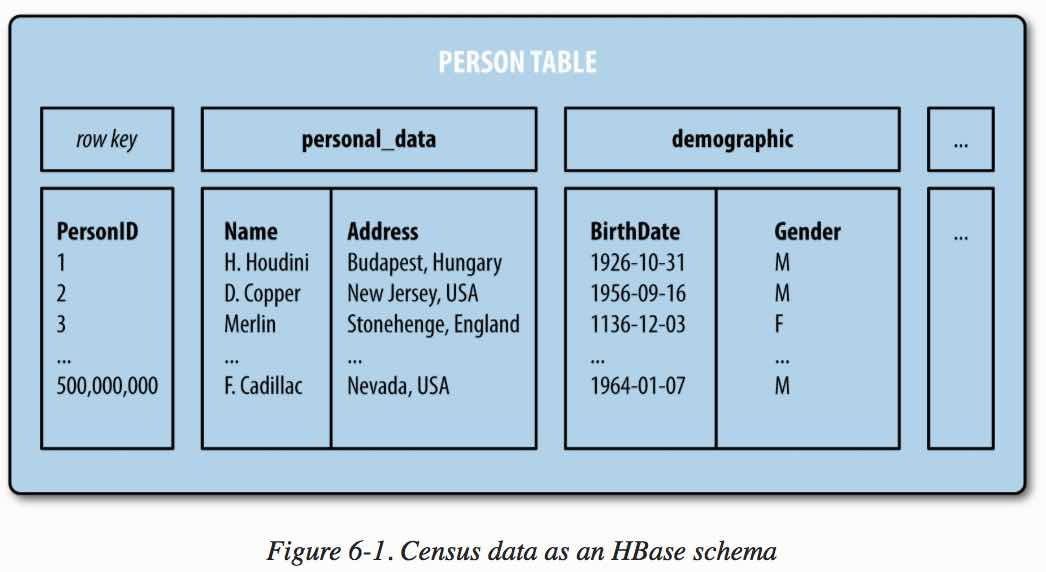
\includegraphics[scale = 0.26]{Immagini/hbasetable.jpg}
\end{figure}
Il modello colonnare non presta attenzione ai \textit{join}, che in questo caso implicherebbero scorrere l'intera tabella, ma si concentra sul \textbf{denormalizzare} ovvero a replicare le informazioni se devo fare dei join tra i vari elementi.\\
Quindi lo schema è formato dalle tables e dalle column family, \textbf{le colonne non fanno parte dello schema}.\\ 
Hbase implementa le \textbf{dynamic Columns} in quanto ogni riga ha differenti colonne.\\ Il versioning è essenziale per garantire lo storico delle informazioni. SU Hbase ho alcune operazioni fondamentali come aggiungere valori e ricercare per valore esatto (e non in modo range-based).\\

Vediamo quindi come si distribuisce un cluster Hbase. Si hanno tre componenti principali (ricordando che si basa su Hadoop), avendo un'architettura master/slave: 
\begin{enumerate}
  \item un master, detto \textbf{HbaseMaster}
  \item tanti region server, detti \textbf{HRegionServer}, che sono i vari slave
  \item il client, detto \textbf{Hbase client}, che dialoga con il singolo master 
\end{enumerate}
Nel dettaglio una \textit{region} è un sottoinsieme di righe della tabella, che vengono partizionate orizzontalmente tramite regole standard di frammentazione (partizionamento che viene fatto in automatico). Quindi un \textit{HRegionServer} gestisce un insieme di righe di una o più tabelle e la sincronizzazione avviene tramite file di log. Il master coordina gli slave, assegna le region, riconosce fallimenti degli slave. \\

Guardando l'intero diagramma il client fa la richiesta al master il quale cerca la posizione del dato e sviluppa l'operazione all'interno della singola region. Nel momento in cui il region server scrive i dati, attraverso il sistema distribuito chiamato \textbf{Hadoop Distributed File System (\textit{HDFS})}, viene fatta la replica e avviene il trasferimento delle informazioni dei file di log e quindi la sincronizzazione dei dati.\\
Potrei avere più master coordinati tra loro. Il coordinamento tra i master e i region server avviene tramite il meccanismo di \textbf{ZooKeeper}, ovvero un orchestratore software. HDFS permette di avere la memorizzazione orizzontale dei dati e tramite il \textbf{write ahead log (\textit{WAL})} prima scrivo sul log e poi sul disco, garantendo la ricostruibilità dei dati in caso di guasto e garantendo che prima o poi i dati saranno allineati. ZooKeeper quindi coordina master e region server per lettura/scrittura mentre HDFS consente l'allineamento dato che poi i dati vengono memorizzati su un file system distribuito.\\ 
Hbase ha un linguaggio di query poco ricco, potendo fare solo una \textit{select} di dati con un certo valore. Si può comunque fare la ricerca sia sulle righe che su alcuni attributi (definiti precedente come chiave). Il sistema di ricerca è estremamente performante.
\subsection{Cassandra}
Come abbiamo detto \textbf{Cassandra} lo studiamo come modello \textit{wide column} anche se loro stessi si definiscono anche \textit{key-value}, essendo sostanzialmente tale ma usando concetti dei modelli \textit{wide column}.\\ Cassandra è l'evoluzione open source del db NoSQL utilizzato da Facebook e risulta interessante perché implementa un sistema di distribuzione completamente diverso da quello master/slave di Hbase.\\ In cassandra esiste il concetto \textbf{column family}, definito all'interno di un \textbf{key space}, come insieme di coppie key-value e quindi una column family altro non è che una tabella con le coppie key-value come righe. Ogni riga ha poi assocciato un $Row Id$ che la identifica.(scritto su slide)\\ Il concetto di column family quindi varia rispetto a quello di Hbase. Una riga è una collezione di colonne con un nome, il $Row id$. La chiave corrisponde al nome della colonna e ogni riga contiene almeno una colonna.\\

Si possono aggiungere attributi a piacere e modificarli (mentre in Hbase si creavano/modificavano le column family). Se i valori corrispondenti a tutte le column name sono uguali a \textbf{-} si specifica che essi non sono usati. Posso anche specificare di avere un singolo valore non in uso sempre con \textbf{-}. Il linguaggio di query di cassandra è chiamato \textbf{Cassandra Query language (CQL)} molto simile ad SQL
\begin{lstlisting}[caption = creazione molto simile al linguaggio SQL si usano infatti gli stessi costruttori]
  CREATE TABLE users(
    email varchar,
    bio varchar,
    birthday timestamp,
    active boolean,
    PRIMARY KEY (email)
  )
\end{lstlisting}
Anche per le query da eseguire usano un modello simile ad SQL dove le \textit{select} leggono uno o più records dalle column family di Cassandra ritornando un insieme di righe: 
\begin{lstlisting}
    SELECT * 
    FROM users; 
    SELECT email 
    FROM users 
    WHERE active = true; 
\end{lstlisting}

La particolarità di Cassandra è l'architettura, in Cassandra si ha un'architettura distribuita \textit{Peer-to-Peer} che si basa sostanzialmente su una modalità simile a \textbf{distributed hash tables (\textit{DHT})}. Cassandra  implementa un meccanismo in cui si garantisce l'\textbf{elasticità} in modo \textbf{trasparente}, aggiungendo i vari nodi in modo molto efficace e performante. Per farlo si prende lo spazio di indirizzamento delle chiavi e si assegna l'organizzazione prendendo lo spazio di indirizzamento, dividendolo nei nodi disponibili. Tramite ZooKeeper si garantisce anche in questo caso la ridondanza, supportando anche la \textbf{rack awareness} (dati possono essere replicati tra diversi rack per proteggersi da guasti di macchine/rack). Inoltre non si ha un \textbf{single point of failure}.\\
Analizzando nel dettaglio il partizionamento si ha che i nodi sono divisi in modo logico in una forma ad anello, detta \textbf{ring topology}. Si usano quindi i valori hash delle chiavi, associate alle partizioni dati, per assegnare la chiave e i dati ad un nodo dell'anello. L'hashing viene limitato ad un certo valore massimo per permettere la struttura ad anello, e si ha che i nodi con meno carico si spostano sull'anello per alleggerire quelli con più carico.

L'aggiunta di un nodo influisce solo sul nodo precedente e il nodo successivo. Spesso i nodi vengono replicati almeno 3 volte e viene fatto nei primi 3 nodi successivi al nodo di cui si sta facendo la replica. Le repliche di un nodo vengono fatte ad ogni scrittura dello stesso. Sapendo che ogni nodo monitora il successivo, qualora questo sia guasto, si può chiedere a quello successivo ancora, garantendo che i dati non vengono persi, il quale a sua volta replicherà su un nodo successivo all'ultimo sui cui aveva repliche per avere sempre le 3 repliche. \\ 
Per monitorare i guasti si usano i \textbf{protocolli gossip}. L'idea è quella che un nodo chiede al successivo e al successivo ancora se sia vada tutto bene, ottenendo, di passaggio in passaggio, una conoscenza completa e robusta dello stato del cluster (ricordando che essendo una rete \textit{Peer-to-Peer} non si ha alcun master). In caso di failure si procede alla riscrittura dei dati sul nodo successivo tramite il file di log.\\ Le operazioni di write sono quindi \textbf{write ahead log}, prima scrivo quindi sul \textbf{commit log} e poi sulla tabella persistente.\\ Parliamo quindi di consistenza dei dati.\\ 

Cassandra nel suo linguaggio offre la possibilità do esguire \textbf{read/write consistency} avendo delle politiche per cui si hanno letture/scritture consistenti:
\begin{itemize}
  \item \textbf{read consistency}: la lettura è data per certa se un nodo risponde, politica \textbf{ONE to ALL} o, altrimenti, se un certo numero di nodi è d'accordo prima di ritornare il risultato della lettura
  \item \textbf{write consistency}: la scrittura è data per certa se se almeno un nodo mi risponde o anche se tutti i nodi rispondono. 
  \item Si ha inoltre una politica di \textbf{quorum} per il calcolo della maggioranza, per la quale anche possono avvenire read/write consistency, che si basa sul \textbf{$\frac{replication \_ factor}{2} + 1$}.
\end{itemize}
La richiesta di consistenza viene fatta nelle query: 
\begin{lstlisting}
    INSERT INTO table (column1,...) 
    VALUES (value1,...) 
    USING CONSISTENCY ONE
\end{lstlisting} 
Dove nel nostro esempio con \texttt{USING CONSISTENCY ONE} si specifica che basta la conferma di un nodo per validare l'operazione. Potrei usare poi \texttt{USING CONSISTENCY QUORUM}, che si basa sul valore $k$ del \textit{$\frac{replication \_ factor}{2} + 1$}, che stabilisce che servono almeno $k$ nodi che validino l'operazione. Con \texttt{USING CONSISTENCY ALL} specifico che tutti i nodi devono confermare l'operazione.\\

Posso avere poi \texttt{USING CONSISTENCY ANY}, specificando anche il booleano \textit{hinted\_handoff\_enable}, che autorizza la scrittura anche se si ha il nodo offline in quanto un'altro nodo prende la richiesta in carico e, non appena il nodo originale torna accessibile, ne trasferisce i dati e il nodo originario procede con la richiesta\\

In merito alle operazioni di \textit{delete} si ha che esse semplicemente rendono il dato non disponibile, essendo più veloce cambiare un flag piuttosto che cancellare. Nel usare questo metodo si creano nelle tabelle fisiche dei problemi di spazio, quindi periodicamente si fanno dei \textbf{merge}, ovvero ogni singolo nodo procede alla compattazione dei propri dati, sovrascrivendo i valori non più disponibili.\\

Per assicurare la sincronizzazione dei nodi e per evitare perdita di consistenza si utilizzano dei \textit{checksum} per comparare i dati di un nodo con quelli dei successivi. Per effettuare questo controllo, nel dettaglio, vengono usati degli hash-tree.\\

Le letture inconsistenti vengono fatte usando \texttt{ANY}, posso poi specificare che mi risponda un nodo con \texttt{ONE} come per le scritture.\\ 
Quindi in lettura, i nodi vengono interrogati fino a quando il numero di nodi che rispondono con il valore più recente non raggiunge un livello di coerenza specificato da \textbf{ONE to ALL}.
% \section{Data Integration}
Si parla solitamente di:
\begin{itemize}
    \item \textbf{data integration}, dove si hanno diversi set di dati (anche non disgiunti) con attributi diversi. Si costruisce un unico insieme con tutti gli elementi dei due insiemi, con gli elementi presenti nell'eventuale intersezione con tutti gli attributi dei due insiemi di partenza . In pratica si fa un \textit{full outer join}. La tecnica di join considerata prende tutti i valori della tabella di sinistra e esegue un match, se possibile, con quelli della tabella di destra. In questo modo si prendono però poi anche tutti gli elementi che non sono collegati con una chiave esterna primaria (non fanno parte del join). Il risultato finale potrebbe non avere dell'informazione in più sui dati.
    \item \textbf{data enrichment}, dove voglio arricchire i dati di un insieme con quelli di altri insiemi, se possibile. In altre parole è una specie di \textit{left outer join}, devo si prendono tutti gli elementi della tabella di sinistra e vengono aggiunte le informazioni della tabella di destra. Questo nel caso in cui ci sia  un match, con i valori della tabella di sinistra, con la tabella di destra. In caso alternativo non aggiungo nulla. Si ha un match diverso dalla semplice uguaglianza tra il set che voglio arricchire e quello che contiene i potenziali arricchimenti. Potrei avere quindi uguaglianza, similitudine o altro, questo perché posso rilassare i vincoli di match quando voglio arricchire l'informazione. Il dataset arricchito contiene quindi solo gli elementi del dataset iniziale che volevo arricchire ma questi potrebbero (potrei non essere riuscito ad arricchire tutti i dati) contenere informazioni in più
\end{itemize}
In entrambi i casi per rappresentare l'assenza di un attributo uso un NULL nella tabella se si parla di un modello relazionale. In caso dei vari modelli NoSQL
seguo gli standard dei vari modelli e dei vari DBMS per rappresentare l'assenza di valore per un certo attributo.\\
Solitamente si cerca di aggiungere, per integrazione o arricchimento:
\begin{itemize}
    \item informazioni spaziali, con informazioni geografiche, o di appartenenza, dei dati che mancano e quindi vanno aggiunte
    \item informazioni temporali, con informazioni storiche dei dati da integrare/arricchire. Si ha però un problema di capire cosa venga prima e cosa dopo, per via della mancanza di timestamp, comportando ambiguità nel rapporto causa-effetto.
\end{itemize}
ma potrebbero esserci infinite altre casistiche.\\

\subsection{Eterogeneità}

Avere un livello di omogeneità facilita l'interazione tra diverse tabelle di un dataset, ma anche di architetture che usano una modalità di relazione diversa. Nel caso in cui siano eterogenei la situazione si complica ancora di più se ho modelli eterogenei, dal punto di vista dei modelli, avendo modelli sia relazionali che non relazioni.

Si hanno vari livelli di eterogeneità/conflitti:
\begin{itemize}
    \item \textbf{eterogeneità di nome}, legato a come sono state etichettate le eterogeneità. Ho quindi concetti di primo livello che rappresentano le stesse informazioni ma con label diverse.
    \item \textbf{eterogeneità di tipo}, ovvero a come modellizzo effettivamente un particolare pezzo della realtà
\end{itemize}
Oltre a questi si ha appunto l'\textbf{eterogeneità di modello} che copre ogni altro tipo di eterogeneo.
\subsubsection{Eterogeneità di nome}
Partiamo con questa prima categoria. Si hanno situazioni di:
\begin{itemize}
    \item \textbf{sinonimia}, ovvero rappresento lo stesso concetto con nomi diversi, che sono sinonimi. Sintassi diversa e semantica uguale.
    \item \textbf{omonimia}, ovvero rappresento concetti diversi con gli stessi nomi. Questo caso è più complicato da riconoscere (ad esempio potrei avere \textit{Città} in due schemi ma in uno rappresenta quella di nascita e in un altro quella di residenza) e rischia di comportare diversi errori, magari portando a dover decidere quale valore associare senza sapere come decidere, integrando in modo errato e perdendo informazione. Raramente si ha accesso alla documentazione dei dataset e quindi bisogna sperare che i vari attributi siano il meno ambigui possibile. Sintassi uguale e semantica diversa
    \item \textbf{iperonimia}, ovvero tra i due concetti uno è più di alto livello rispetto all'altra, secondo magari una relazione \textit{IS-A}.
\end{itemize}
\subsubsection{Eterogeneità di tipo}
In questo caso si ha che lo stesso concetto viene rappresentato in modo strutture concettualmente diverse in due schemi, potendo quindi avere, ad esempio:
\begin{itemize}
    \item domini di definizione differenti per lo stesso attributo in due schemi (ad esempio da una parte il dominio delle città italiane e dall'altro quelle  islandesi)
    \item un attributo in uno schema e avere un valore derivato in un altro schema, avendo quindi, nel primo caso, un attributo indipendente mentre nel secondo si ha una dipendenza funzionale con un altro attributo
    \item un attributo in uno schema e un entità in un altro schema 
    \item un attributo in uno schema e una gerarchia di generalizzazione in un altro schema 
    \item un'entità in uno schema e una relazione in un altro schema o magari, nel modello a grafo, avendo in uno schema un nodo e un arco nel secondo
    \item diversi livelli di astrazione per lo stesso concetto in due schemi (ad esempio due entità con nomi omonimi legati da una gerarchia IS-A in due schemi)  
    \item diverse granularità nei domini di definizione 
    \item diverse cardinalità nelle stesse relazioni 
    \item key conflicts (la chiave in uno schema è diverso da quella dell'altro)
\end{itemize}

\subsubsection{Data integration system}
Succede quindi che si ha una \textbf{trasformazione di schema}. Si procede con uno \textbf{schema matching} per capire come unificare i vari schemi per ottenere uno schema integrato omogeneo. Questo si fa capendo quali attributi coincidono anche se magari si presentano con sintassi diverse. \\
Il software che procede con queste fasi è detto \textbf{data integration system} che procede prendendo e mettendo insieme delle sorgenti dati e cerca di ottenere uno schema integrato. Vengono presi e uniti tutti gli attributi degli schemi.\\ \textit{In modo analogo funzionano i datawarehouse dove ho schemi diversi, solitamente relazionali ma non sempre, che vengono messi insieme e quindi manipolati}.\\

Ci sono diversi approcci che si possono utilizzare, infatti abbiamo una vera e propria classificazione delle varie tecniche, per eseguire il schema matching in modo da avere uno schema integrato immediato. Spesso bisogna fare schema matching \textit{on the fly} dovendo integrare nuovi schemi in modo assai rapido. Si hanno anche sistemi su grande scala con sistemi \textit{pay as you go}, dove serve altrettanta velocità.\\

Ci sono diverse fasi da eseguie:
\begin{enumerate}
    \item \textbf{schema transformation o pre-integration}, è una fase quindi propedeutica che presi in input $n$ schemi me li restituisce omogenei tramite tecniche di model trasformation o reverse engineering. 
    \item \textbf{Correspondences investigation}, dove si studiano le corrispondenze tra gli schemi tramite tecniche specifiche
    \item \textbf{schemas integration e mapping generation}, dove si definiscono lo schema integrato e le regole di mapping necessarie
\end{enumerate}
Per la fase di pre-integration, vediamo che  avendo da integrare/arricchire decine di schemi si hanno diverse strategie. Si hanno due scelte fondamentali:
\begin{enumerate}
    \item integro a coppie. Grazie a questa scelta binaria ho due possibilità:
        \begin{enumerate}
            \item prendere uno schema, integrarlo con un altro e integrare il risultato con un altro ancora etc$\ldots$. Ottengo una soluzione a scala con un albero binario non bilanciato
            \item uso un approccio bilanciato aggregando schemi vicini e aggregando poi i vari risultati delle integrazioni. Ottengo quindi un albero binario bilanciato 
        \end{enumerate}
    \item integro con più schemi contemporaneamente. Ho due approcci:
        \begin{enumerate}
            \item integrare tutti gli schemi insieme (\textbf{questo bisogna evitarlo} anche solo per $n>3$, si dovrebbero considerare tutte le permutazioni e non è facile)
            \item integrare in modo iterativo, in modo analogo a quanto fatto con il bilanciamento binario ma ovviamente non con un numero fisso di schemi da integrare ogni volta (magari ne integro due o magari tre, raramente di più per ovvi motivi)
        \end{enumerate}
\end{enumerate}

Invece per la seconda fase, quella di \textbf{Correspondences investigation}, si ha appunto anche il problema che posso dire le stesse cose con strutture completamente diverse. Si cercano quindi \textbf{corrispondenze semantiche} sfruttando la conoscenza pregressa sul dominio applicativo. Si possono sfruttare sia le \textbf{equivalenze}, ovvero componenti con gli stessi nomi (attenzione anche se hanno lo stesso nome possono rappresentare informazioni diverse), che le \textbf{generalità} (\textit{IS-A}) per cercare le eventuali corrispondenze. Si rischia di avere anche \textbf{disgiunzioni} tra attributi completamente diversi magari di schemi uguali rischiando di avere problemi.\\ 

Passiamo alla fase dinale, di \textbf{schemas integration e mapping generation}, ci serve capire come generare le regole di associazione. In uno schema non relazionale identificare i mapping è quindi molto arduo ma bisogna anche generare i nuovi mapping e le nuove regole di associazione.\\ Classificando i matching si trovano anche nuove tipologie di conflitto che devono essere risolti con trasformazioni opportune. Dobbiamo quindi meglio definire in primis i conflitti.
Si hanno diversi tipi di conflitti:
\begin{enumerate}
    \item \textbf{conflitti di classificazione} quando elementi omologhi descrivono insiemi diversi di oggetti del mondo reale. Si risolve tramite generalizzazione o specifica della gerarchia.
    \item \textbf{conflitti descrittivi} quando tipi omologhi hanno proprietà diverse o le stesse proprietà sono descritte diversamente. Si hanno:
        \begin{itemize}
            \item conflitti di nome, ovvero nomi diverse per le stesse cose
            \item conflitti di composizione, ovvero diversi attributi e/o metodi (magari avendone di più o di meno o anche diversi)
        \end{itemize}
    La soluzione dipende dai casi sulla base del tipo di conflitto incontrato e il tipo di classificazione del conflitto. 
    \item \textbf{conflitti strutturali} dove si hanno gli stessi elementi rappresentati tramite strutture diverse (magari da una parte un elemento è un'intera entità e dall'altra solo un attributo). Per risolvere si sceglie, per massimizzare l'informazione ottenuta, di prendere la struttura meno vincolata. Questo si fa per aumentare il volume delle informazioni.  
    \item \textbf{conflitti di frammentazione} dove magari lo stesso elemento è rappresentato da un singolo oggetto in uno schema mentre è rappresentato da diversi oggetti in un secondo database. Si integrano i dati quindi anche nell'ottica di rimetterli insieme.
\end{enumerate}

Parliamo quindi delle \textbf{regole di mapping} definite tra gli schemi di partenza e quelli ottenuti dopo l'integrazione. 
Si possono trovare, per lo schema di partenza $S$, osservando le trasformazioni effettuate per la risoluzione di omologie e conflitti avuti durante il processo di integrazione. Le regole mi dicono che un elemento chiamato in un modo nello schema integrato ha una precisa corrispondenza con un certo elemento di uno schema sorgente.\\
Se si hanno conflitti a livello direttamente di istanze, avendo che li stessi dati (lo stesso oggetto del mondo ideale) in sorgenti diversi hanno valori diversi, i problemi aumentano. Questo è un problema fondamentale nel data integration, anche nel caso dell'arricchimento. \\
Posso avere:
Date due sorgenti $S_1$ e $S_2$, siano $A_{1k}$ e $A_{1k}$ i valori che associati ad un attributo, rispettivamente, $t_1$ di $S_1$ e $t_2$ di $S_2$, abbiamo
\begin{itemize}
  \item un \textbf{conflitto di attributi} avendo due entità che rappresentano lo stesso oggetto reale con attributi diversi (anche solo uno) per la stessa proprietà. Le chiavi in questo caso sono coerenti. Occorre quindi se $A_{1k} \neq A_{1k}$
  \item un \textbf{conflitto di chiave} (detto anche \textbf{conflitto di entità \textnormal{o} conflitto di tupla}) se ho chiavi primarie diverse in due entità diverse che però rappresentano lo stesso oggetto mentre gli altri attributi coincidono
\end{itemize}
Una scelta di soluzione, detta \textbf{currency}, prevede, in caso di conflittualità di valore di attributo, di scegliere il valore inserito temporalmente per ultimo, nella speranza che sia il più aggiornato (ma spesso non è esattamente così). Le tecniche che trattano i conflitti a livello di istanza possono essere applicate in due diverse fasi del ciclo di vita di un sistema di integrazione dati, vale a dire:
\begin{itemize}
  \item a \textbf{design time}
  \item a \textbf{query time}
\end{itemize}
In entrambi i casi i conflitti saltano fuori a query time. Tuttavia, durante il design time si decide la strategia da seguire per risolvere i conflitti prima che le query vengano elaborate, ovvero nella fase di progettazione del sistema di integrazione dei dati. Le tecniche che operano a query time incorporano le specifiche della strategia da seguire all'interno della formulazione della query. 
Si hanno quindi le \textbf{funzioni di risoluzione dei conflitti} che prendono in input due valori conflittuali e hanno come output la risposta della query effettuata. Un criterio di misura si basa sull'affidabilità delle sorgenti stesse da cui proviene il conflitto. In altri casi si ragiona in termini di funzioni matematiche di minimo, massimo, media, varianza e altri concetti matematici, ma questo in presenza di valori numerici. Per valori non numerici si hanno altre funzioni, ad esempio la concatenazione nel caso di stringhe o la scelta delle più lunghe/corte. Ovviamente non si può sapere la risposta giusta ma si può imporre una logica di stima. È comunque buona pratica tenere traccia tali conflitti e in caso siano troppi preoccuparsi dell'effettiva validità dei dati. Il data integration assume due forme:
\begin{enumerate}
  \item \textbf{deduplicazione}, dove si scopre se ci sono concetti del mondo reale replicati nella tabella, avendo che l'integrazione viene fatta solo su quella tabella (non avendo schema matching), internamente. 
  \item integrazione in due tabelle diverse, avendo schema matching. Si supponga quindi di voler fondere due tabelle senza chiave primaria. Si cerca quindi una pseudo-chiave primaria (usando l'insieme più grande di attributi comuni alle tabelle che siano significativi, ad esempio nome, cognome e luogo di nascita) matchando le tabelle su di essa. Ma potrei anche qui non matchare per errori di scrittura. Faccio quindi un matching approssimato e concatenando le due tabelle e procedendo poi con la deduplica della tabella risultante. Potrei comunque sempre ragionare con la distanza di edit etc$\ldots$ restando con le tabelle separate, procedendo con una combinazione lineare degli score delle distanze (riscalate su $\{0,1\}$, con 1 match perfetto, facendo una somma pesata e dividendo per il numero di score), decidendo una soglia oltre la quale si ha il match. Si usano tecniche probabilistiche. 
\end{enumerate}

Si sono finora trascurati quei casi in cui si sta palesemente rappresentando la stessa cosa ma con termini diversi (magari con nomi contratti, esempio Leonardo che diventa Leo.). Si ha infatti il \textbf{record linkage}, ovvero la tecnica di risoluzione dei conflitti a livello di istanza, dove, date le tabelle in input, posso avere in output:
\begin{itemize}
  \item \textbf{matching tuples}, ovvero i valori che sicuramente matchano (anche se non perfetti ma con score oltre una certa soglia)
  \item \textbf{non matching tuples}, ovvero i valori che sicuramente non matchano
  \item \textbf{possible matches}, ovvero una sorta di area grigia dove non si sa come dare risposta. La scelta della soglia per il match e di quella per il non match, se scelta con valori dubbi, si avrà come conseguenza che molti casi siano dubbi, essendo quest'area quella compresa tra le due soglie.
\end{itemize}
In mezzo subentra l'umano che \textbf{a mano} sistema i valori, non avendo altro modo. Da qualche anno si è anche introdotto il machine learning, tramite \textbf{Deepr} per sostituire l'uomo nell'analisi di questa zona di mezzo. Le soluzioni di machine learning sono fortemente legate al dominio. \\

Si è dato per scontato un altro problema: le dimensione delle tabelle. In quel caso il check dei valori tra le tabelle esplode nel numero di confronti. Bisogna quindi ridurre lo \textbf{spazio di ricerca}, non potendo fare il prodotto cartesiano tra le tabelle ($ A\times B$), per via dei valori che ci si ritrovioamo a ricavare, quindi non è una soluzione che integra la \textbf{scalabilità}. \\
Vediamo quindi quali sono gli step che si incontrano eseguendo un \textbf{record linkage probabilistico}:
\begin{enumerate}
  \item \textbf{preprocessing}, normalizzazione dei formati (espansione abbreviazioni, lowercase, eliminazione spazi e caratteri speciali o passando ad altre codifiche, come la geocodifica) secondo uno standard
  \item \textbf{blocking}, riduzione dello spazio di ricerca. 
  \item \textbf{compare}, scegliendo una funzione di distanza e cercando un sample con coppie conosciute di match e unmatch. Per ogni caso calcolare il valore della distanza per frequenza di matching e unmatching.
  \item \textbf{decide}, valutando la distanza e le soglie
\end{enumerate}

Per la fusione posso:
\begin{itemize}
  \item ignorare un conflitto, mettendo tutti i valori disponibili
  \item cercare di evitare i conflitti basandomi sui metadati, sul sorgente o sulle istanze  
  \item gestire i conflitti tramite le funzioni di risoluzione dei conflitti e alle altre cose discusse sopra
\end{itemize}

Si hanno elenchi delle varie strategie possibili (ignorare, scegliere il più recente, scegliere il valore medio e molte altre), ognuna delle quali, come anche il record linkage, può introdurre errori. La scelta delle soglie inoltre può portare ad essere meno conservativi, introducendo falsi positivi, o troppo conservativi, riducendo drasticamente i match. Le varie scelte dipendono comunque dai singoli casi.
% \section{Data Integration Architectures}
Le lezioni principalmente si baseranno sulla \textbf{verifica della qualità} dei dati, sulla \textbf{pulizia} e \textbf{integrazione} dei dati.
Si parte come abbiamo detto da una serie di schemi separati in vari database, con modelli diversi. Posso avere anche file excel, quindi fogli csv. Bisogna quindi raccogliere le varie informazioni e integrarle in un unico dataset. Si hanno più tecniche, noi andiamo a vedere:
\begin{itemize}
  \item la tecnica del \textbf{consolidamento} dove si raccolgono vari dataset dalle varie sorgenti informative, li integro come visto precedentemente (tecniche di data integration) e infine salvo il risultato in un nuovo file o in un database.
  \item la tecnica che prevede di rappresentare i vari schemi separati in modo che essi siano mantenuti inalterati, non memorizzando il risultato dell'integrazione, ma dando possibilità all'utente di scrivere query \textit{on the fly} sui dati integrati. Questo è la vera e propria tecnica di \textbf{virtual data integration}
\end{itemize}
%%ATTENZIONE, SI RIRPORTANO SLIDE E SPIEGAZIONE, MAGARI CI SONO ERRORI RIP
\textbf{Nelle lezioni fornite ci andiamo a occupare principalmente di virtual data integration anche se spesso non specificato}.\\
Il data integration è un è un'importante area di ricerca e business che ha lo scopo principale di consentire ad un utente un accesso uniforme a più fonti di dati autonome ed eterogenee, attraverso la rappresentazione di una visione unificata dei dati. Trovare questa uniformità tra elementi eterogenei è complesso perché bisogna trovare differenze e somiglianze in ogni schema per potersi conformare. Bisogna quindi riconciliare tutte le eterogeneità di schema e di istanza.\\ 

Il vantaggio di architetture d'integrazione rispetto alle architetture federate è la capacità di gestire meglio le eterogeneità, soprattutto se complesse, a livello di schema. Inoltre i sistemi federati non possono gestire eterogeneità a livello di istanze a causa di errori di qualità (che possono essere rappresentati da accuratezza, incompletezza, inconsistenza o altri fattori) presenti dati. Nelle architetture federate si ha un livello di autonomia in poco più basso nel senso che nei modelli integrati si assume che si hanno sorgenti provenienti da chissà dove mentre nei sistemi federati i nodi sono scelti in modo più consapevole.\\

Si hanno due approcci principali alla data integration (due classi di appalcazione):
\begin{enumerate}
  \item La più importante è la \textbf{integrated read-only views Mediation}: dove si ha integrazione solo per lettura. I dati letti nei vari database restano quindi invariati. Questa soluzione a livello aziendale viene scartata in favore delle datawarehouse, avendo persistenza dei dati e profondità storica maggiore (anche se perdo flessibilità nel momento in cui si rimuove una sorgente dati).
  \item \textbf{integrated read-write views Mediation with update}, dove si hanno anche gli update. È estensione dell'architettura di Mediation per supportare gli aggiornamenti in favore di una vista integrata. Questa cosa è difficile e anche poco studiata in letteratura e quindi non la tratteremo. In questo caso si preferiscono i modelli federati.
\end{enumerate}
L'integrazione dei dati è il problema di combinare i dati che risiedono in sorgenti diverse e fornire all'utente una visione unificata di questi dati può quindi essere letteralmente definita come \textbf{global virtual schema (GS)}.\\ 
Parto dai vari database coi vari modelli e schemi e creo un GS che ha un certo modello. Si hanno mapping tra i vari schemi e il GS e quindi l'utente può effettuare delle query passando per il GS, a runtime il GS capisce dove sono le informazioni richieste. Esegue una trasformazione dal linguaggio usato per la query in quello necessario per il database dove si trova l'informazione ed effettua la query sul database localmente. Sempre on the fly si risolvono i conflitti e viene restituito il risultato della query. Potrei avere anche integrazione \textbf{pay as you go}.\\
Si hanno quindi tre elementi fondamentali in un'architettura di integration: il global scheme, le varie sorgenti locali e il mapping tra le sorgenti e il GS.

Si hanno quindi due componenti fondamentali:
\begin{enumerate}
  \item vari \textbf{wrapper}, che agganciano ogni schema locale con lo schema globale (GS), consentendo di rappresentare la sorgente in uno schema compatibile con quello del GS. I wrapper devono ricevere query nel linguaggio del modello dello schema globale e rispondono di conseguenza. Ovviamente se serve esegue la traduzione. 
  \item un \textbf{mediator}, che data una query la frammenta e la riscrive per poter eseguire le interrogazioni ai vari schemi locali. Inoltre il mediator mette insieme i vari risultati, risolve i conflitti e risponde alla query.
\end{enumerate}

Le architetture \textbf{wrapper-mediator} sono lo standard nel mondo del virtual data integration, nel dettaglio della \textbf{lazy integration}. L'integrazione è pigra perché non c'è una materializzazione dei dati, né in fase di consolidamento né in fase di datawarehouse e che consente una maggior flessibilità rispetto ai dati. Infatti se all'interno di una risorsa sorgente aggiungo un nuovo valore, il \textbf{mediator} la vede immediatamente. \\ Bisogna studiare GS e mapping.\\ 
Si hanno due tipiche architetture del sistema, a seconda della direzione dei mapping:
\begin{enumerate}
  \item una in cui si parte dagli schemi locali per arrivare al GS
  \item una in cui si parte dal GS e si arriva gli schemi locali
\end{enumerate}
In ogni caso lo scopo è interrogare l'informazioni come se fosse unica.\\

La funzionalità principale di un mediator è la riconciliazione delle istanze. Una volta effettuata la parte di discesa, dalla query dell'utente verso query locali, fino a quando i database locali costruiscono una risposta. A questo punto si costruisce uno schema unificato di diverse fonti di informazioni e questo consente a un utente di formulare una query su di esso. La query dell'utente viene quindi trasformata in una serie di sottoquery, una per ciascuna fonte di dati coinvolta nella query e il risultato viene sempre raccolto e unificato dal mediator che lo restituisce all'utente.\\ 
Il mediator quindi deve riconciliare le varie istanze mettendo insieme le varie risposte dei vari database. Si hanno varie azioni, da svolgere in breve tempo (essendo tutto on the fly), fatte dal mediator:
\begin{itemize}
  \item raggruppare informazioni sulla stessa entità del mondo reale 
  \item rimuovere la replicazione dei tra le varie fonti di dati 
  \item risolvere le inconsistenze tra le varie fonti di dati 
  \item ottenere accuratezza, completezza, etc$\ldots$ tra i dati provenienti da diverse fonti di dati   
\end{itemize}
L'interazione con il mediator è quindi divisa in due fasi:
\begin{enumerate}
  \item la creazione della rappresentazione unificata creando uno schema globale oppure di eseguire mapping (\textbf{Publishing phase at design time}),
  \item una fase eseguita a runtime che consiste nella la formulazione e l'esecuzione di una query nella rappresentazione unificata (\textbf{Querying Phase}).
\end{enumerate}

Nella fase di \textbf{publishing} i problemi sono quelli di modellare e andare a definire  dei linguaggi per lo schema unificato, devo inoltre rappresentare i mapping. Nel caso, solo se si usano architetture con update, gestire anche quest'ultimo. Abbiamo un'estrazione dagli schemi sorgenti.
Nella fase di \textbf{querying} bisogna stabilire il linguaggio, fare query unfloding/rewriting grazie ai mapping. Devo inoltre, durante la fase di risalita, cleaning e fusion dei risultati. Bisogna inoltre convertire i vari linguaggi da GS a schemi locali.\\ 

Il mapping è centrale in entrambi. Possiamo vedere il sistema di virtual data integration come una tripla: $(G,S,M)$ dove:
\begin{itemize}
  \item $G$ indica lo schema globale
  \item $S$ l'insieme degli schemi sorgente
  \item $M$ il mapping
\end{itemize}
I dati risiedono quindi nelle sorgenti, le query del sistema unificato vengono espresse utilizzando il linguaggio usato nello schema globale, queste specificano anche di quali dati, presenti ora nel nostro database virtuale, siamo interessati. Dobbiamo appunto costruire uno schema globale virtuale. Il problema è capire quali dati reali nelle sorgenti di dati corrispondono a quei dati virtuali rappresentati per mezzo dallo schema globale. \\ %nn o ben capito
Per il mapping si hanno vari approcci, a seconda della relazione tra lo schema globale e quelli locali, rispetto al concetto di vista (che in SQL ricordiamo costruire una sorta di tabella virtuale):
\begin{itemize}
  \item \textbf{GAV (Global As View)}, in cui lo schema globale viene creato sulla base dell'osservazione degli schemi sorgente, attraverso un processo di integrazione intensionale degli schemi sorgenti (si pensi anche al processo di consolidamento, o ad una situazione in che vogliamo rappresentare in modo integrato tutto il contenuto informativo dell'architettura dati di un'organizzazione). In questo caso lo schema globale è espresso in termini di schemi locale. L'approccio si può riassumere dicendo che lo schema globale è una vista degli schemi locali (tutte, contemporaneamente). In questo caso il mapping va dagli schemi locali a quello globale. Il vantaggio è che si prendono tutte le informazioni disponibili, non scelgo quali sono gli elementi siano o meno rilevanti, procedo tramite arricchimento dei dati ma potrebbe capitare che non si ottiene lo schema voluto, questo perché i dati non le lo consentono.\\
  
  GAV ha dei problemi nel caso si abbiano da gestire degli update in caso di rimozione in quanto tutti i concetti che prima avevano a che fare con la sorgente tolta vanno cambiati, avendo poi problemi anche a livello di istanze (questo non succede in caso di aggiunta, in quel caso semplicemente rifaccio l'integrazione e aggiungo elementi allo schema globale, anche se questo ha un costo). Questo approccio ci dice come recuperare i dati da istanze di origine locale (reale) per ciascuna tabella dello schema globale (virtuale). Con il GAV il mediatore procede tramite unfloding delle query, cioè la sostituzione nella query dei riferimenti allo schema globale con l'espressione della view globale in termini delle view locali.
 
  \item \textbf{LAV (Local As View)}, dove lo schema globale viene progettato a priori indipendentemente dagli schemi sorgente, da cui prenderò solo i pezzi di informazione di interesse. Il mapping tra le sorgenti e lo schema globale si ottiene definendo ciascun sorgente sullo schema globale. Può capitare che un concetto dello schema locali non sia rappresentato nello schema globale, questo non è importante, infatti a noi importa che per ogni concetto globale avrà una qualche rappresentazione locale. \\
  
  Questo approccio rende più semplice l'evoluzione temporale dello schema globale in quanto in caso di update aggiungendo uno schema locale non cambia lo schema globale (che è fisso), ma si ha solo un eventuale arricchimento del mapping con un nuovo query mapping. \\
  
  Il mapping va quindi dallo schema globale a quelli sorgente/locali avendo che il contenuto di ogni schema locale è descritto in termini di vista sullo schema globale. Se una colonna non è presente nel globale ma solo nel locale rispondo \textbf{NULL}. 
  \item \textbf{GLAV (Global and Local As View)} dove il mapping tra sorgenti e schema globale si ottiene definendo un insieme di viste, alcune sullo schema globale e altre sulle origini dati. È un approccio ibrido.
\end{itemize}


\section{Data quality}
Un esempio di scarsa data quality è quella di avere lo stesso dato con valori diversi nello stesso posto, anche semplicemente una pagina web.\\ 
I dati sono una rappresentazione della realtà e questo porta al fatto che la realtà viene da noi modellata tramite alcuni dati specifici. Si definiscono quindi:
\begin{itemize}
  \item \textbf{utilità} come precisione della rappresentazione interna del dato rispetto a il compito svolto (e quindi, ad esempio, un'immagine ritoccata potrebbe essere più utile per determinati scopi, si vede meglio anche attraverso la nebbia)
  \item \textbf{fedeltà} su come una determinata interpretazione aderisce al mondo reale
\end{itemize}
\subsection{Concetti Fondamentali}
Alcuni dei concetti fondamentali, che vengono appresi e che sono un punto di riferimento, quando si parla di qualità dei dati sono:
\begin{itemize}
    \item \textbf{qualità}: caratteristiche di un artefatto che influiscono sulla sua capacità di soddisfare le esigenze e le aspettative dell'utente, dichiarate o implicite. Un dato è di qualità se è adatto all'uso che se ne vuole fare. Si ha il concetto di \textbf{fitness for use}. \textit{ La qualità dei dati è negli occhi di chi li usa e non nelle mani di chi li produce.}
    \item \textbf{dimensione}(o caratteristica): una caratteristica specifica che descrive la qualità delle informazioni associato al dato, solitamente non misurabile. Alcune volte è viene misurata, li dimensioni come le sottodimensioni attraverso le \textit{metriche}.
    \item \textbf{sottodimensioni}: sotto-caratteristiche che spesso classificano una certa dimensione.
\end{itemize}
Le metriche sono una procedura che spesso mi consentono di misurare un certo valore. Rifacendoci alle slide ci riferiamo alla definizione presente nello standard ISO 9126-1 e secondo il framework ISM3. Quello che emerge è che le metriche racchiudono sia:
\begin{itemize}
    \item una procedura (o metodo) di misurazione, ad esempio un algoritmo che prende l'elemento da misurare e lo associa a una misura (sia esso un valore ordinale o un intervallo) 
    \item che una corretta unità di misura (o scala), cioè il dominio dei valori restituiti dalla procedura di misurazione
\end{itemize}
Si possono avere metriche diverse per la stessa dimensione.

\subsection{Le dimensioni di qualità dei dati}
La qualità dei dati è un concetto che può essere espresso attraverso molteplici dimensioni, ad esempio la accuratezza (magari anche solo per errori di typo nei dati), la comprensibilità, la completezza (avendo magari valori a NULL), l'inconsistenza e altro.\\

Un altro aspetto da tenere in considerazione è che si hanno metriche:
\begin{itemize}
  \item \textbf{oggettive}, modi formali e precisi per misurare le metriche per una dimensione di qualità in termini di valori di un dominio, indipendentemente dalla percezione/valutazione umana
  \item \textbf{soggettive}, modi per misurare le metriche per una dimensione di qualità che dipendono dalla percezione (di solito valutazione esplicita e ordinale) delle persone coinvolte nel processo di misurazione, dipendente dalla percezione/valutazione umana
\end{itemize}
\subsection{Data quality dimensions}
Si hanno diverse dimensioni e metriche; vengono di seguiuto trattate (sottosezioni)
\subsubsection{Accuratezza}
La precisione di un valore $v$ è definita come la vicinanza tra $v$ e un valore $v'$, questo viene considerato come la corretta rappresentazione del fenomeno del mondo reale che $v$ intende rappresentare. Si può applicare alle tuple e alle relazioni.\\

Si hanno due sottodimensioni di questa qualità:
\begin{enumerate}
  \item \textbf{accuratezza sintattica}, magari controllando se la stringa, inserita in un oggetto o una tupla, è presente in un insieme di valori di riferimento per il dominio trattato (magari un vocabolario, una lista di città etc$\ldots$). Ci sono dati su cui non è applicabile. Generalmente si fa in base alle stringhe oppure in base ai singoli token di una stringa.
  \item \textbf{accuratezza semantica}, molto difficile da verificare (magari tramite un'altra sorgente dati per cross validare). Per piccolissimi db si fa a mano ma è generalmente impensabile. 
\end{enumerate}
Conoscere lo schema aiuta a valutare la accuratezza dei valori e si hanno diverse metriche. Posso verificare se un dato è vicino a quello che mi aspetto in un certo dominio tramite una funzione di distanza che confronta il valore che ho e il dominio di riferimento. Dopo questo posso pensare a correggere eventualmente il dato. Si cerca il valore più vicino al dominio di riferimento.\\

Potrei anche fare una stima statistica per capire quale sia il valore corretto. Per il calcolo delle distanze su stringhe uso la solita \textbf{distanza di edit}, ci sono altri metodi ma useremo questa per ora. In fase di assessment considero solo valori con una massima distanza di edit stabilita e nella fase di improvement posso stimare la giusta correzione per ottenere la stringa magari corretta. \\

La distanza sintattica potrebbe però essere poco informativa in merito alla semantica (si pensi a Domenico spesso abbreviato in Mimmo). Possiamo introdurre la \textbf{distanza di edit normalizzata} come: \[1-\frac{edit(a,b)}{n}\] con $n$ numero massimo di simboli. Si ottiene un valore tra 0 e 1, con 1 che indica che i valori che sono identici, accuratezza pari a uno implica distanza nulla (misuro il complemento a 1 della distanza). Tali valori tra 0 e 1 sono comodi in quanto spesso le metriche danno risultati che sono in questo range e posso quindi effettuare una somma pesata tra le varie metriche.\\
Si hanno vari tipi di funzione di edit (ma limitate a stringhe corte):
\begin{itemize}
  \item Hamming distance
  \item Levenshtein distance
  \item Jaro-Winkler
\end{itemize}
o di distanza di token (per stringhe composte da più stringhe, esempio ``Sesto San Giovanni''):
\begin{itemize}
  \item Jaccard index
  \item Sorensen-Dice
  \item N-gram
\end{itemize}
Si possono avere problemi nel trovare la reference table di un certo dominio. 
\subsubsection{Completezza}
La completezza riguarda ogni tipo di rappresentazione del dato. Definiamo la \textbf{completezza} (di un insieme di dati) come la copertura con la quale il fenomeno osservato è rappresentato nell'insieme di dati. Avere ad esempio dei NULL impedisce la completezza.\\ Impatta valori alfanumerici e numerici e si può applicare alle tuple, agli attributi, agli oggetti e alle relazioni.\\
Tipicamente si esegue una sottrazione in termini di $1-$ in modo da poter rappresentare la massima completezza a 1:
\begin{itemize}
    \item la completezza di \textbf{tupla}, che identifica la presenza di valori NULL in una tupla, è basata sul numero di NULL di una certa riga rispetto al numero di attributi presenti
    \item la completezza di \textbf{attributo}, che presenta valori NULL all'interno delle colonne di una tabella. è basata sul numero di NULL di una certa colonna rappresentante un attributo
    \item la completezza di \textbf{tabella} è basata sul numero di NULL dell'intera tabella 
    \item la completezza di \textbf{oggetto} è il numero di valori non nulli in tutti gli oggetti rappresentati nelle tuple 
\end{itemize}

Nelle precedenti definizioni, abbiamo assunto una ipotesi di \textbf{mondo chiuso}, ovvero tutto ciò che è rappresentato nella base di dati è vero, tutto il resto è falso. Questa è la tipica ipotesi che si fa nei DBMS. Una ipotesi alternativa è quella di un \textbf{mondo aperto}, come nei DBMS NoSQL, dove di tutto ciò che non è rappresentato non si sa nulla. In questo caso introduciamo la \textbf{object completness}, che tiene conto del fatto che gli oggetti rappresentabili sono più delle tuple della tabella, e di tale cardinalità serve una stimma indiretta. Quindi nel mondo non relazionale è difficile stimare la completezza, non avendo certezza del numero di oggetti.
\subsubsection{Currency}
Una delle \textbf{proprietà temporali}, di livello di aggiornamento, ovvero di \textbf{currency}.\\
Difficile parlare di proprietà temporali perché dare una definizione di tempo risulta difficile,e in secondo luogo bisogna avere ben presente la semantica della dimensione di qualità che dobbiamo considerare.\\
Si ha che la \textbf{currency} misura con quale rapidità i dati sono aggiornati rispetto al corrispondente fenomeno del mondo reale. Una prima misura della currency è il ritardo temporale tra il tempo $t_1$ dell’evento del mondo reale che ha provocato la variazione del dato, e l’istante $t_2$ della sua registrazione nel sistema informativo ma questa misura è costosa in quando generalmente l'evento non è ben noto.\\

Un'altra metrica di currency è vederla come come differenza tra tempo di arrivo alla organizzazione e tempo in cui è effettuato l’aggiornamento (cosa misurabile in presenza di log degli arrivi e degli update). Un'altra metrica è la differenza rispetto al metadato ultimo aggiornamento effettuato che, per valori con periodicità di aggiornamento nota, currency calcolabile in maniera approssimata ma poco costosa (ma non si hanno informazioni in merito alle modifiche del dato). \\

La \textbf{tempestività} misura quanto i dati sono aggiornati rispetto a un particolare processo (o ai processi) che li utilizza. Questa tecnica, al contrario della currency, è dipendente dal processo,  ed è associabile al momento temporale in cui deve essere disponibile per il processo che utilizza il dato. Posso avere dati obsoleti per il processo di chi li usa ma con alta currency.

\subsubsection{Consistenza}
Si definisce la \textbf{consistenza} in due modi:
\begin{enumerate}
    \item come consistenza dei dati con i vincoli di integrità o dipendenze funzionali definiti sullo schema (ad esempio i vincoli di integrità nel modello relazionale).\\
    Si hanno anche dei vincoli di consistenza, detti business rule, che possono riguardare uno o più attributi, relazioni o altro. Possono essere espressi in termini di probabilità. Si usano anche vincoli di integrità in logica e si hanno dei data edit nelle indagini statistiche
    \item come consistenza delle diverse rappresentazioni di uno stesso oggetto della realtà presenti nella base di dati
\end{enumerate}

\subsubsection{Accessibilità}

Invece con \textbf{accessibilità} si esprime la capacità di un utente di accedere ai dati a partire dalla propria cultura, stato fisico e psichico e dalla tecnologie disponibilità. Un altro aspetto importante che va sempre considerato è il \textbf{tradeoff tra varie qualità}, ad esempio consistenza e completezza nel modello relazionale possono essere non conciliabili quando si voglia rispettare l'integrità referenziale. Nel dominio statistico si ha tradeoff tra tempestività e completezza/accuratezza, che vengono però privilegiate (bisogna quindi studiare quanto è sporco un certo dato). Nel web si preferisce la tempestività rispetto ad accuratezza/completezza.
\section{Quality improvement}
Avendo quindi già introdotto la fase di \textbf{quality assesment} passiamo a quella di \textbf{quality improvement}, ovvero al miglioramento dei dati stessi.\\ L'obiettivo della fase di miglioramento, una volta misurata la qualità dei dati mi accorgo che i dati sono di bassa qualità rispetto alle esigenza, si deve cercare  di migliorare i dati. La qualità dei dati è un problema di tipo multidimensionale, potendo decidere di migliorare anche solo alcuni aspetti relativi alla qualità dei dati (come la completezza, la consistenza, l'aggiornamento temporale). Sappiamo inoltre che ci sono dei tradeoff quindi il miglioramento di alcuni aspetti va a discapito della qualità di altri. Si hanno in generale due strategie in fase di miglioramento:
\begin{enumerate}
    \item \textbf{data-driven}, migliorando il dato stesso in quanto tale. Si punta a migliorare la qualità dei dati modificando direttamente il valore dei dati attraverso il confronto con altri dati ritenuti di buona qualità. Ad esempio, i valori dei dati obsoleti vengono aggiornati aggiornando un database caratterizzato da una currency, quindi da una misura eseguita attraverso una metrica temporale, più alta. Si migliora il dataset stesso.\\ Si hanno varie procedure:
        \begin{enumerate}
            \item \textbf{acquisizione di nuovi dati}, migliora i dati attraverso l'acquisizione di dati di qualità alta che andranno a sostituire i valori che sollevano problemi di qualità. Questa strategia può essere utilizzata per tutte le dimensioni esaminate nella fase di valutazione (assessment)
            \item \textbf{record linkage}, detta anche \textbf{identificazione degli oggetti}, che confronta i dataset, che contengono valori sporchi, con una fonte certificata o di qualità superiore, identificando le tuple/record nei due dataset che potrebbero fare riferimento allo stesso oggetto del mondo reale. In seguito si va eseguire una \textit{pulizia} dei dati sporchi in favore dei dati con qualità più alta.
            \item \textbf{affidabilità della fonte}, dove si selezionano le fonti di dati sulla base della qualità dei loro dati
        \end{enumerate}
    \item \textbf{process-driven}, migliorando il processo di acquisizione dei dati (datti errati possono portare ad errori sistematici), ottenendo che il dataset viene alimentato con dati corretti. Si punta quindi a migliorare la qualità ridisegnando i processi che creano o modificano i dati. Ad esempio, un processo può essere riprogettato includendo un'attività che controlla il formato dei dati prima della loro archiviazione. Tale strategia fa riferimento all'ambito detto \textbf{Business Process Reengineering (BPR)}, ovvero avendo la possibilità di riprogettare i processi, magari scoprendo che una sorgente era di qualità troppo bassa.\\
    Si hanno due tecniche:
        \begin{enumerate}
        \item \textbf{process control}, dove si aggiungono elementi e/o procedure di controllo nel processo di produzione dei dati quando: vengono creati nuovi dati, vengono aggiornati i set di dati o il processo accede a nuovi set di dati.
        Verificando errori e la qualità dei dati stessi.\\
        In questo modo, viene applicata una strategia reattiva, che quindi agisce tempestivamente, agli eventi di modifica dei dati, evitando così la degradazione dei dati e la propagazione degli errori.
        \item \textbf{process redesign}, dove si ridisegnano i processi per rimuovere le cause della scarsa qualità e introduce nuove attività che producono dati di qualità più alta. Se la riprogettazione del processo è radicale, questa tecnica viene definita \textit{business process reengineering}.
        \end{enumerate}
    Queste tecniche sono puntuali e non sono facilmente integrabili in un sistema di raccolta continua dei dati.
\end{enumerate}

Nel lungo termine le tecniche process-driven sono più efficaci, eliminando il problema alla radice, ma sono estremamente costose nel breve termine. Le tecniche data-driven sono più economiche ma costose nel lungo e quindi sono adatte per un'applicazione one-shot, solitamente sono consigliate per i dati statici. \\

Si hanno miglioramenti specifici per la dimensione:
\begin{itemize}
    \item \textbf{accuratezza} tramite confronto dei valori con un dominio di riferimento. Questo è il tipo di tecnica che abbiamo considerato per l'accuratezza sintattica nella fase di quality assesment.
    \item \textbf{completezza} tramite completamento di dati incompleti con tecniche specifiche che sfruttano la conoscenza sui dati.
    \item \textbf{consistenza} tramite l'identificazione dei dati corretti sfruttando vincoli di integrità, dipendenze funzionali o dati derivati, in quale modo posso poi andare a correggere i miei dati tramite sorgenti esterni o acquisendo nuovamente i dati.
\end{itemize}

\textit{Sulle slide è segnata come "d", ma ti giuro che non solo non c'è la "c", ma non ci sono nemmeno "a" e "b". Apparso a caso, magari se capisci dove collocarlo dimmi rip. Inoltre poi abbimao la deduplica che è un punto 3, ma esiste solo il punto 1, che questo error cose sia il punto 2 e non il d?????}\\

Come tecnica si usa anche la \textbf{error localization and correction} che identifica ed elimina gli errori di qualità dei dati rilevando i valori che non soddisfano un dato insieme di regole, dette \textbf{edits}. Queste tecniche sono principalmente studiate nel dominio statistico.
Rispetto ai dati elementari, i dati statistici aggregati (Da wiki: Le aggregazioni di dati sono dati di alto livello composti da una moltitudine, o da una loro combinazione, di dati individuali.) (come media, somma, massimo).
Questi dati sono meno sensibili alla localizzazione probabilistica e alla correzione dei valori probabilmente errate. Sono state proposte tecniche per la localizzazione e correzione degli errori per incongruenze, dati incompleti e valori anomali, ovvero valori significativamente diversi da tutti gli altri valori in un set di dati per dati elementari e dati statistici.\\

Un altra tecnica di quality improvement è la \textbf{deduplica} che corrisponde al raggruppamento di record di dataset che si riferiscono alla stessa entità nel mondo reale (raggruppo i doppioni). Praticamente la deduplica è un'operazione di record linkage fatta su un'unica tabella. La tabella risultate è strutturata in modo tale da avere le tuple suddivise in 3 gruppi:
\begin{enumerate}
    \item coppie/gruppi di tuple che matchano, corrispondenti allo stesso oggetto reale
    \item coppie di tuple che non matchano che corrispondono a entità distinte nel mondo reale 
    \item possibili coppie/gruppi di tuple, per le quali non è stato possibile giungere una conclusione definitiva, e sono necessarie ulteriori indagini (e costi) per assegnarle al gruppo match o mismatch
    
\end{enumerate}
Un'altra attività classica, propedeutica ad altre attività (è una sorta di fase di preprocessamento), è la fase di \textbf{normalizzazione}, trasformando le stringhe, scritte nello standard del dominio di riferimento, effettuando per ogni dimensione, il riconoscendo della stessa e il relativo miglioramento. Si ha quindi il miglioramento di singoli valori o di intere tuple, migliorando accuratezza sintattica, completezza, currency e consistenza, in base a certe metriche. \\ 

Ogni valore che non matcha con la tabella di riferimento (spesso disponibili online a seconda del dominio ma non sempre) deve essere corretto. Il miglioramento dell'accuratezza sintattica viene effettuato sostituendo il valore errato con quello a distanza inferiore nella tabella di riferimento, dove la distanza può essere valutata dopo una precedente verifica dei valori e delle loro caratteristiche (si nota come le attività data-driven sono costose dal punto di vista temporale). \\

Mentre per migliorare l'accuratezza possiamo adottare procedure standard di confronto con le tabelle di riferimento, per la completezza è molto più complesso. Non avendo un elemento da cui partire, avendo a disposizione solo un valore NULL, non sempre si riesce a ricostruire il valore corretto per sostituirlo al NULL. Spesso comunque si ha un contesto per aiutare a rimuovere i NULL. La procedura più intuitiva è eseguire una nuova acquisizione di dati incompleti riempiendo di volta in volta più valori NULL possibili. Poiché di solito si tratta di un'attività molto costosa, possiamo adottare diverse euristiche che di solito dipendono dal contesto. \\ 

Per la completezza si usano anche i \textbf{dati derivati}, definiti come dati per i quali esiste una formula matematica per la quale questi dati possono essere ottenuti a partire da un altro set di dati già conosciuto.\\ 
Bisogna migliorare la consistenza vedendo se la dipendenza funzionale sui dati derivati e altri vincoli di integrità intra-relazionale possono essere sfruttati, oltre che per la completezza completezza, anche per la consistenza.\\ 

Dopo tutte queste operazioni si ottiene un db già abbastanza pulito ma si hanno, solitamente, ancora problemi con spazio di miglioramento. Si userà quindi il \textbf{record linkage}.
\section{Record linkage}
Il \textbf{record linkage} viene usato anche in altri contesti oltre il data quality con anche altri nomi (come deduplicazione, se si tratta di un solo dataset). \\ 
Prima della fase di data integration si ha lo \textit{scheme integration}, con approcci architetturali. Dal punto di vista di integrazione si hanno, si ricorda, gli approcci GAV o LAV, ma in entrambi i casi si hanno elementi rappresentanti lo stesso oggetto reale in db diversi che potrebbero non essere facilmente  integrati a causa, magari, dell'assenza di una chiave primaria univoca. Bisogna quindi studiare come collegare i record presenti nei vari db tramite \textbf{record linkage} e mettere poi insieme i risultati con un'operazione di \textbf{fusion}, cercando di studiare eventuali ridondanze o ambiguità.\\ 

Il record linkage consiste quindi nell'identificare le stesse osservazioni in diversi file/db. In generale si parla di \textbf{entity resolution task/record linkage} avendo varie varianti:
\begin{itemize}
    \item \textbf{deduplicazione}, che considerando una sola tabella è usata principalmente con il modello ER. Si procede raggruppando record che corrispondono allo stesso oggetto reale normalizzando lo schema e riducendo il numero di record nel dataset. Come variante si hanno i cluster di calcolo
    \item \textbf{record linkage}, dove appunto si matchano da un archivio dati deduplicato a un altro (bipartito). Si ha anche la versione $k$-partita lavorando con più data store. Generalmente questo metodo proposto nei datastore relazionali, ma più frequentemente applicato a record non strutturati da varie fonti
    \item \textbf{canonicalizzazione}, che generalmente fornisce il record più completo, attribuisce i valori tramite la fusione, costruendo dei \textbf{single version of truth}, usando metodi probabilistici. Questo metodo è tipico nel \textit{master data management}, dove si raccolgono tutti i dati per poi integrarli
    \item \textbf{referencing}, detto anche \textbf{entity disambiguation}, dove si matchano record sporchi con uno pulito, con una tabella di riferimento deduplicata che è già stata canonizzata. Questo metodo generalmente utilizzato per atomizzare più record sulla stessa chiave primaria e donare informazioni aggiuntive al record
\end{itemize}

Si hanno vari tool per la entity resolution:
\begin{itemize}
    \item \textit{NTLK}, un natural language toolkit
    \item \textit{Dedupe*}, per lo structured deduplication
    \item \textit{Distance}, un'implementazione in C per distance metrics
    \item \textit{Scikit-Learn}, per machine learning models
    \item \textit{Fuzzywuzzy}, per fuzzy string matching
    \item \textit{PyBloom}, per probabilistic set matching
\end{itemize}

In input al record linkage si ha quindi una serie di tabelle e in output un insieme di tuple che matchano e un insieme di tuple che non matchano, nel caso relazionale. Si hanno anche tuple per cui non si sa dire nulla o per le quali non si ha certezza su match/mismatch. Lo stesso ragionamento si applica anche a modelli non relazionali\\
Si hanno varie tecniche per la comparazione delle coppie:
\begin{itemize}
    \item quella \textbf{empirica}, basata sulla distanza di simboli, dal punto di vista lessicografico, nei valori delle tuple (Crlo è simile a Carlo)
    \item quella \textbf{probabilistica}, dove presumo di conoscere un campione di frequenze di distanze tra coppie di tuple, note come corrispondenti o non corrispondenti e dove potrei decidere quelli corrispondenti e quelli non corrispondenti nell'universo proiettando tale conoscenza sul campione nell'universo della coppia. Si usano soglie per poter discernere match e mismatch
    \item quelle \textbf{knowledge based}, dove si decide in base a regole per il match delle tuple
    \item \textbf{mista}, sia probabilistica che knowledge based 
    \item le recenti tecniche di \textbf{machine learning}
\end{itemize}
Ovviamente grosse tabelle portano, confrontando tutti gli elementi ogni volta, una alta complessità, dal punto di vista prestazionale inefficienti. Si hanno quindi vari step per il record linkage:(non ho capito se parla solo di tabelle)
\begin{itemize}
    \item costruzione dello spazio di ricerca iniziale come prodotto cartesiano di tutti i dataset in input.Questa è una fase di preprocessamento e in questa fase si cerca di ottenere un formato unico per tutti i sorgenti, sia dal punto di vista del modello che da quello dei dati (normalizzando i vari valori di uno stesso dominio, ad esempio avendo un solo modo per definire la via, di non usare abbreviazioni) 
    \item si usano tecniche di blocking per ridurre lo spazio di ricerca, ottenendo uno spazio di ricerca ridotto. Si hanno varie tecniche di blocking in letteratura e vari algoritmi. Tra tutti si ha il \textit{sorted neighbour} dove si prende un attributo e cerco di ordinare la tabella sugli insiemi degli attributi in modo tale che i gruppi degli attributi che confronto siano vicini tra loro. 
    
    Ci si muove tra gli elementi tramite sliding window per specificare meglio i controlli, riducendo i confronti (senza la finestra ho $n^2$ confronti, con $n$ righe, con la finestra di lunghezza $m$ righe ho $m^2\frac{n}{m}$, quindi $m\cdot n$ confronti, avendo $m\ll n$). Questa fase è facilmente distribuibile, facendo finestre di controllo in parallelo i più nodi 
    \item sullo spazio ridotto si usa un metodo di comparazione, a cui è associato un metodo di decisione, per definire i match, i mismatch e quelli di cui non si ha certezza, che chiamiamo possible match (non sempre si hanno, dipende dalle soglie usate, una soglia di certo non permette di creare i possible match due invece si, nel mezzo tra le due si hanno i possible match). Si hanno metodi probabilistici, metodi non supervisionati come il clustering e anche supervisionati come:
    svm, logistic, random forest, boosting gradient.  Confrontando quindi le varie coppie di dati
\end{itemize}
Questo è lo schema di base e in ogni fase si ha un processo di quality assesment.\\
Il primo problema è che i dataset potrebbero essere di formato diverso, relazionale o meno, e quindi, come i data integration, si cerca di trasformare un modello nell'altro. Potrei dover unire in un unico formato anche immagini e mappe, oltre a documenti json o csv.\\ 

Approfondiamo quindi l'uso di tecniche \textbf{probabilistiche} per la fase di comparazione, avendo un \textbf{probabilistic record linkage}, dove comunque le prime fasi restano normali. Quindi si cerca la probabilità di match tra le coppie usando dei vettori di distanza, usando la somma pesata dei vettori: 
\[P_{match}=\sum_{score\in A}w\cdot score\]
Avendo:
\begin{itemize}
  \item $w$ pesi tra 0 e 1, avendo peso maggiore per feature meglio predittibili
  \item $A$ vettore degli attributo ciascuno con un punteggio $score$
\end{itemize}
Se il punteggio così pesato supera una soglia ottengo un match.\\ Si hanno anche meccanismi basate su regole, sebbene la loro formulazione sia difficile, è possibile applicare regole specifiche del dominio rendendo più specifico l'approccio.\\ La soluzione proposta da \textbf{Fellegi Sunter}, quella probabilistica, è ottimale quando gli attributi di confronto erano condizionatamente indipendenti, permettendo comunque di avere un'area di ambiguità date dalla distribuzione dai match/mismatch.\\ 

Bisogna quindi per ogni coppia definire una funzione di distanza, imponendo un insieme finito di attributi da usare per valutare tale distanza, potrebbero esserci attributi non rilevanti. Un modo ottimale è scegliere attributi dello stesso significato e con la maggior accuratezza possibile per evitare errori. Si hanno anche attributi discriminatori per i quali i domini contengono un alto numero possibile di valori. Meno attributi si prendono in considerazione più rischio falsi positivi, aumentando i matching, anche se aumento le prestazioni. Scegliere troppi attributi può portare a falsi negativi, avendo tantissimi mismatch. È quindi un discorso che va approfondito di caso in caso.\\

L'algoritmo di Fellegi Sunter, per la fase decisionale, suggerisce di campionare la frequenza di match e non match, prendendo una coppia che si sa già che matcha e valutando per ogni distanza la frequenza di match/mismatch andando a calcolare in seguito la probabilità di match in base alla percentuale di match/mismatch dati dalla distanaza di edit (ex: distanza di edit =2, abbiamo 27 match e 12 mismatch, la percentuale è 27/(27+12)=70\%). Si fa un ragionamento in stile SVM anche se senza iperpiani ma con un separatore più complesso.\\

All'aumentare della distanza ovviamente aumentano i mismatch e viceversa. Alla fine del ragionamento posso produrre le soglie (o la soglia) da usare per lo studio dell'intero dataset.  Si rischiano comunque falsi positivi e falsi negativi che possono essere ridotti aumentando i possibile match, allargando le soglie. Il record linkage, nel calcolo della distanza, è comunque molto legato al dominio.\\ 

Approfondiamo ora le tecniche di comparazione basate sul machine learning. Si hanno approcci supervisionati, SVM, random forest, conditional random fields e altri. \\ 
Ci sono anche tecniche non supervisionate, tramite clustering, con l'idea di usare K-means per raggruppare elementi simili.\\ Matchare testi descrittivi lunghi è difficile ma con tecniche di distanza non euclidea e di embedding, in un contesto comunque di machine learning, si riesce ad ottenere dei risultati.\\ In generale comunque il record linkage deve essere veloce, anche a discapito di un minimo di qualità.\\
Bisogna quindi valutare la qualità in termini di: true positive (TP), true negatives (TN), false positive (FP) e false negative (FN); ripotando le notazioni di recall e precisione dei dati:
\[recall=\frac{TP}{TP+FN} \qquad precision=\frac{TP}{TP+FP}\]
Avendo un'elevata conoscenza di dominio posso usare tali conoscenze per la comparazione e la cosa è difficilmente generalizzabile.

\subsection{Data fusion}
Passiamo quindi alla fusione dei record che rappresentano lo steso oggetto nel mondo reale. Bisogna gestire i conflitti. Si hanno varie tecniche:
\begin{itemize}
    \item \textbf{ignorare il conflitto}, non è una buona soluzione. Queste strategie non consentono di prendere la decisione in base a ciò che è in conflitto con i dati e a volte non vengono rilevati i conflitti di dati.
    \item \textbf{evitare il conflitto}, con strategie basate su istanze e metadati, scegliendo di prendere istanze senza conflitti, prendendo solo valori consistenti senza dire niente degli altri.
    \item \textbf{risolvere il conflitto}, prendendo una sorgente più sicura o facendo una scelta a basata su vari aspetti. La decisione tiene conto o dei metadati o delle singole istanze per valutare la strategia. Si hanno due strategie:
        \begin{enumerate}
        \item decidere quando scegliere un valore tra tutti i valori già presenti
        \item strategie di mediazione, quando scelgono un valore che non necessariamente esiste tra i valori inconsistenti (ad esempio faccio la media tra due valori per fare non avere conflitti(instance based) oppure prendere il valore più aggioranto (metadata based))
    \end{enumerate}
\end{itemize}
La scelta di fusione deve essere comunicata a chi poi usa i dati altrimenti si rischiano molti problemi. 

È il tema della \textbf{provenance dei dati}, il tenere traccia delle decisioni prese. Con al data fusion si ottiene potenzialmente qualcosa con pochi NULL.\\ Alcune note con conclusive.\\ La \textbf{data preparation} è un buon modo per ottenere ottimi risultati, tramite normalizzazione di dati e schemi e \textit{imputation}. Si rendono più facili i riscontri tramite distanze sintattiche.
\end{document}
